
% XXX- discuss GtkBin; which widgets have a window, which do not --image and label do not, and we mightwant them too,
%   modify_bg() only affects widgets that have an associated gtk.gdk.Window.
% > Widgets that do not have an associated window include .... gtk.Arrow,
% > gtk.Bin, gtk.Box, gtk.Button, gtk.CheckButton, gtk.Fixed , gtk.Image ,
% > gtk.Label , gtk.MenuItem , gtk.Notebook , gtk.Paned , gtk.RadioButton ,
% > gtk.Range , gtk.ScrolledWindow , gtk.Separator , gtk.Table , gtk.Toolbar ,
% > gtk.AspectFrame , gtk.Frame , gtk.VBox , gtk.HBox , gtk.VSeparator ,
% > gtk.HSeparator . These widgets can be added to a gtk.EventBox to overcome
% > this limitation.




%% RGtk2 chapter
\chapter{RGtk2: Overview}
%%\section{Introduction}
\label{sec:RGtk2-Introduction}
%% intorduction

%% Technical, but short beginning

As the name implies, the \pkg{RGtk2} package provides a connection, or
bindings, between \GTK\/ and \R\/ allowing nearly the full power of
\GTK\/ to be available to the \R\/ programmer. In addition,
\pkg{RGtk2} provides bindings to other libraries accompanying \GTK:
The Pango libraries for font rendering; the Cairo
libraries for vector graphics; the GdkPixbuf libraries for image
manipulation; libglade for designing GUI layouts from an XML
description; ATK for the accessiblity toolkit;  and GDK, which
provides an abstract layer between the windowing system, such as X11,
and \GTK. These libraries are multi-platform and extensive and have been
used for many major projects, such as the linux versions of the
firefox browser and open office.

% Actually, the bindings to GTK are only part of the story. RGtk2 also
% offers complete bindings to Pango (font rendering), GDK (basic
% drawing, low-level device access), Cairo (vector graphics), GdkPixbuf
% (image manipulation), libglade (GUI's from XML descriptions),
% GtkMozEmbed (embeddable mozilla browser on linux), and ATK
% (accessibility devices). [Michael Lawrence's announcement]


\pkg{RGtk2}, for the most part, automatically creates \R\/ functions
that call into the \GTK\/ library. For example, the \R\/ function
\function{gtkContainerAdd} eventually calls the C function
\code{gtk\_container\_add}. The naming convention is the C name has its underscores
removed and each following letter capitalized (camelback).


The full API for \GTK\/ is quite large, and clearly can not be
documented here. However, the \GTK\/ documentation is converted into
\R\/ format in the building of \pkg{RGtk2}. This conveniently allows
the programmer to refer to the appropriate documentation within an
\R\/ session, without having to consult  a web page, such as
\url{http://library.gnome.org/devel/gtk/stable/}, which lists the API
of the stable versions \GTK.



%%% ------- OOP --------------

\section{How \GTK\/ is organized}
\label{sec:RGtk2:constructors}


\GTK\/ objects are created using constructors such as
\function{gtkWindowNew} and \function{gtkButtonNewWithLabel} (these
mapping to \code{gtk\_window\_new} and
\code{gtk\_button\_new\_with\_label} respectively). \pkg{RGtk2} also
provides constructors with names not ending in ``\code{New}'' that may,
depending on the arguments given, call different, but similar,
constructors. As such we prefer the shorter named constructors, such as
\function{gtkWindow} or \function{gtkButton}.

\subsection{Methods}


%% OO methods
The underlying \GTK\/ library is written in C, but still provides a a
singly inherited, object-oriented framework that leads naturally to
the use of S3 classes for the \R\/ package. In \GTK\/ the
\class{GtkWindow} class inherits methods, properties, and signals from
the \class{GtkBin}, \class{GtkContainer}, \class{GtkWidget},
\class{GtkObject}, \class{GInitiallyUnowned}, and \class{GObject}
classes. In \pkg{RGtk2}, we can see the class heiarchy by calling
\function{class} on a \command{gtkWindow} instance:~\footnote{We use
  the term ``instance'' of a constructor to refer to the object
  returned by the constructor, which is an instance of some class.}
\begin{Schunk}
\begin{Sinput}
 class(gtkWindow())
\end{Sinput}
\begin{Soutput}
[1] "GtkWindow"         "GtkBin"            "GtkContainer"     
[4] "GtkWidget"         "GtkObject"         "GInitiallyUnowned"
[7] "GObject"           "RGtkObject"       
\end{Soutput}
\end{Schunk}

The classes are identical except for the addition of the base \class{RGtkObject}
class. When a widget is destroyed, the \R\/ object is assigned
\class{<invalid>} class.

Methods of \pkg{RGtk2} do not use S3 dispatch, but rather an internal
one. The call \code{obj\$method(...)} resolves to a function call
\code{f(obj,...)}. The function is found by looking for any function
prefixed with with either an interface or a class from the object
followed by the method name. The interfaces are checked first.

For instance, if \code{win} is a \function{gtkWindow} instance, then to resolve the call
\code{win\$add(widget)} (or \code{win\$add(widget)}) \R\/ looks for methods with the name
\function{gtkBuildableAdd}, \function{atkImplementorIfaceAdd},
\function{gtkWindowAdd}, \function{gtkBinAdd} before finding
\function{gtkContainerAdd} and calling it as
\code{gtkContainerAdd(win,widget)}. The \method{\$}{GObject} method for \pkg{RGtk2} objects does the
work. Understanding this mechanism allows us to add to the \pkg{RGtk2}
API, as convenient. For instance, we can add to the button API with

\begin{Schunk}
\begin{Sinput}
 gtkButtonPrintHello <- function(obj) print("hello")
 b <- gtkButton()
 b$printHello()
\end{Sinput}
\begin{Soutput}
[1] "hello"
\end{Soutput}
\end{Schunk}

%% common methods
Some common methods are inherited by most widgets, as they are defined
in the base \class{gtkWidget} class. These include the methods 
\method{Show}{gtkWidget} to specify that the widget should be drawn;
\method{Hide}{gtkWidget} to hide the widget until specified;
\method{Destroy}{gtkWidget} to destroy a widget and clear up any
references to it; \method{getParent}{gtkWidget} to find the parent
container of the widget; \method{ModifyBg}{gtkWidget} to modify the
background color of a widget; and \method{ModifyFg}{gtkWidget} to
modify the foreground color.


\subsection{Properties}


%% --------- Properties ------------
Also inherited are widget properties. A list of properties that a
widget has is returned by its \method{GetPropInfo}{gObject}
method. \pkg{RGtk2} provides the \R\/ generic \method{names}{Gobject}
as a familiar alternative for this method. For the button just
defined, we can see the first eight properties listed with:
\begin{Schunk}
\begin{Sinput}
 head(names(b), n=8)                     # or b$getPropInfo()
\end{Sinput}
\begin{Soutput}
[1] "user-data"      "name"           "parent"         "width-request" 
[5] "height-request" "visible"        "sensitive"      "app-paintable" 
\end{Soutput}
\end{Schunk}

Some common properties are \code{parent} to store the parent widget
(if any); \code{user-data} which allow one to store arbitrary data
with the widget; \code{sensitive}, to control whether a widget can
receive user events;


There are a few different ways to access these properties. Consider
the \code{label} property of a \code{gtkButton} instance.  \GTK\/
provides the functions \function{gObjectGet} and \function{gObjectSet}
to get and set properties of a widget.  The set funtion using the
arguments names for the property key.

\begin{Schunk}
\begin{Sinput}
 b <- gtkButton("A button")
 gObjectGet(b,"label")
\end{Sinput}
\begin{Soutput}
[1] "A button"
\end{Soutput}
\begin{Sinput}
 gObjectSet(b,label="a new label for our button")
\end{Sinput}
\end{Schunk}
Additionally, most user-accessible properties have specific \code{Get} and
\code{Set} methods defined for them. In our example,  the methods
\method{getLabel}{gtkButton} and \method{setLabel}{gtkButton} can be used.
\begin{Schunk}
\begin{Sinput}
 b$getLabel()
\end{Sinput}
\begin{Soutput}
[1] "a new label for our button"
\end{Soutput}
\begin{Sinput}
 b$setLabel("Again, a new label for our button")
\end{Sinput}
\end{Schunk}

\pkg{RGtk2} provides the convenient and familiar \code{[} and
\code{[$<$-} methods to get and access the properties:
\begin{Schunk}
\begin{Sinput}
 b['label']
\end{Sinput}
\begin{Soutput}
[1] "Again, a new label for our button"
\end{Soutput}
\end{Schunk}

For ease of referencing the appropriate help pages, we tend to use the
full method name in the examples, although at times the move \R-like
vector notation will be used for commonly accessed properties.

%%% ------ constants --------

\subsection{Enumerated types and flags}


The \GTK\/ libraries have a number of constants that identify
different states. These enumerated types are defined in the C
code. For instance, for a toolbar, there are four possible styles: with
icons, just text, both text and icon, and both text and icon drawn
horizontally. The flags indicating the style are stored in C in an
enumeration \code{GtkToolbarStyle} with constants
\code{GTK\_TOOLBAR\_ICONS}, \code{GTK\_TOOLBAR\_TEXT}, etc. In \pkg{RGtk2}
these values are conveniently stored in the vector
\code{GtkToolbarStyle} with named integer values
\begin{Schunk}
\begin{Sinput}
 GtkToolbarStyle
\end{Sinput}
\begin{Soutput}
     icons       text       both both-horiz 
         0          1          2          3 
attr(,"class")
[1] "enums"
\end{Soutput}
\end{Schunk}

A  list of enumerated types for \GTK\/ is listed in the man
page \code{?gtk-Standard-Enumerations} and for \code{Pango} in
\code{?pango-Layout-Objects}. The \code{Gdk}  variables are
prefixed with \code{Gdk} and so can be found using \function{apropos},
say, using \code{ignore.case=TRUE}.

To use these enumerated types, one can specify them by name as
\begin{Schunk}
\begin{Sinput}
 tb <- gtkToolbar()
 tb$setStyle(GtkToolbarStyle['icons'] )
\end{Sinput}
\end{Schunk}

But \pkg{RGtk2} provides the convenience of specifying the style name
only, as in
\begin{Schunk}
\begin{Sinput}
 tb$setStyle("icons")
\end{Sinput}
\end{Schunk}

When more than one value is desired, they can be combined using
\function{c}.

%%% ------ Signals ----------

\subsection{Events and signals}


In \pkg{RGtk2} user actions, such as mouse clicks, keyboard usage,
drag and drops, etc. trigger \pkg{RGtk2} widgets to signal the action.
A GUI can be made interactive, by adding callbacks to respond when
these signals are emitted. In addition to signals, there are a number
of window manager events, such as a \code{button-press-event}. These
events have callbacks attached in a similar manner.

The signals and events that an object adds are returned by the method
\method{GetSignals}{gObject}. For example
\begin{Schunk}
\begin{Sinput}
 names(b$getSignals())
\end{Sinput}
\begin{Soutput}
[1] "pressed"  "released" "clicked"  "enter"    "leave"    "activate"
\end{Soutput}
\end{Schunk}
shows the ``clicked'' signal in addition to others.

To list all the inherited signals can be achieved using
\function{gtkTypeGetSignals}. For instance, the following code will print
out all the inherited signals and events.
\begin{Schunk}
\begin{Sinput}
 types <- class(b)
 lst <- sapply(head(types,n=-1), gtkTypeGetSignals)
 for(i in names(lst)) { cat(i,"\n"); print(lst[[i]])}
\end{Sinput}
\end{Schunk}



%% the gSignalConnect function
\paragraph{Binding a callback}
The \function{gSignalConnect} (or \function{gSignalConnect}) function is used
to add a callback to a widget's signal. Its signature is
\begin{Schunk}
\begin{Sinput}
 args(gSignalConnect)
\end{Sinput}
\begin{Soutput}
function (obj, signal, f, data = NULL, after = FALSE, user.data.first = FALSE)  
\end{Soutput}
\end{Schunk}

The \argument{obj}{gSignalConnect} is the widget the callback is attached to and
\argument{signal}{gSignalConnect} the signal name, for instance \code{"drag-drop"}. 
This may also be an event name.

The \argument{f}{gSignalConnect} argument is for the callback.
Although, it can be specified as an expression or a call, our examples
always use a function to handle the callback. More detail follows. The
\argument{after}{gSignalConnect} argument is a logical indicating if
the callback should be called after the default handlers (see
\command{?gSignalConnect}).

The \argument{data}{gSignalConnect} argument allows arbitrary data to be
passed to the callback.  The \argument{user.data.first}{gSignalConnect} argument
specifies if this \argument{data}{gSignalConnect} argument should be the first
argument to the callback or (the default) the last. As the signature of
the callback has varying length, setting this to \code{TRUE} can prove
useful.

%% the callback
The signature for the callback varies for each signal and 
window manager event. Unless the default for \code{user.data.first} is overridden, the
argument is the widget. For signals, other arguments are
possible depending on the type. For window events, the second argument is a
\class{GdkEvent} type, which can carry with it extra information about
the event that occurred. The \GTK\/ API lists each argument. 

As the callback is an \R\/ function, it is passed copies of the
object. Since \pkg{RGtk2} objects are pointers, there is no practical
difference. So changes within the body of a callback to \pkg{RGtk2}
objects are reflected outside the scope of the callback, unlike
changes to most other \R\/ objects.


\begin{Schunk}
\begin{Sinput}
 w <- gtkWindow(); w['title'] <- "test signals"
 x <- 1; 
 b <- gtkButton("click me"); w$add(b)
 ID <- gSignalConnect(b,signal="clicked",f = function(widget,...) {
   widget$setData("x",2)
   x <- 2
   return(TRUE)
 })
\end{Sinput}
\end{Schunk}
Then after clicking, we would have

\begin{Schunk}
\begin{Sinput}
 cat(x, b$getData("x"),"\n") # 1 and 2
\end{Sinput}
\begin{Soutput}
1 2 
\end{Soutput}
\end{Schunk}

Callbacks for signals emitted by window manager events are expected to
return a logical value. Failure to do so can cause errors to be
raised. For other callbacks the return value is ignored, so it is safe to
always return a logical value. When it is not ignored, a return value
of \code{TRUE} indicates that no further callbacks should be called,
whereas \code{FALSE} indicates that the next callback should be
called. So in the following example, only the first two callbacks are
executed when the user presses on the button.

\begin{Schunk}
\begin{Sinput}
 b <- gtkButton("click")
 w <- gtkWindow()
 w$add(b)
 id1 <- gSignalConnect(b, "button-press-event", 
                       function(b, event, data) {
                         print("hi"); return(FALSE)
                       })
 id2 <- gSignalConnect(b, "button-press-event", 
                       function(b, event, data) {
                         print("and"); return(TRUE)
                       })
 id3 <- gSignalConnect(b, "button-press-event", 
                       function(b, event, data) {
                         print("bye"); return(TRUE)
                       })
\end{Sinput}
\end{Schunk}

%% multiple callbacks; remove; block
Multiple callbacks can be assigned to each signal. They will be
processed in the order they were bound to the signal.  The
\function{gSignalConnect} function returns an ID that can be used to
disconnect a callback if desired using
\function{gSignalHandlerDisconnect} or temporarily blocked using
\function{gSignalHandlerBlock} and
\function{gSignalHandlerUnblock}. The man page for
\function{gSignalConnect} gives the details on this, and much more.


%% --------- Event Loop

\subsection{The eventloop}


The \pkg{RGtk2} eventloop integrates with the \R\/ event loop. In practice, such
integration is tricky. In a C program, \GTK\/ programs call the
function \code{gtk\_main} which puts control of the GUI into the main
event loop of \GTK. This sits idle until some event occurs. According
to the \pkg{RGtk2} website, ``The nature of the R event loop prevents
the continuous execution of the GTK main loop, thus preventing things
like timers and idle tasks from executing reliably. This manifests
itself when using functionality such as GtkExpander and
GtkEntryCompletion.''

During a long calculation, the GUI can seem unresponsive. To avoid
this the following construct can be used during the long calculation
to process pending events.

\begin{Schunk}
\begin{Sinput}
 while(gtkEventsPending()) 
   gtkMainIteration()
\end{Sinput}
\end{Schunk}



\section{RGtk2 and gWidgetsRGtk2}
\label{sec:RGtk2:gWidgetsRGtk2}


The widgets described above, are also available through
\pkg{gWidgetsRGtk2}. The two packages can be used together, for the
most part. The \code{add} method of \pkg{gWidgetsRGtk2} can be used to
add an \pkg{RGtk2} widget to a \code{gWidgetsRGtk2}
container. Whereas, the \code{getToolkitWidget} method will (usually)
return the \pkg{RGtk2} component to use within \pkg{RGtk2}.

%% Views example in next chapter?

\chapter{RGtk2: Basic Components}
\label{sec:top-level-windows}

\XXX{ --- GDkWindow role (events, coloring, event box): explain on need
to know basis}

\XXX{SetDecorated for gtkWindow}


This section covers some of the basic widgets and containers of
\GTK. We begin with a discussion of top level containers and box
containers. Then we continue with describing many of the simpler
controls -- essentially those without an underlying model, and then
finish by describing a few more containers. 

\section{Top-level windows}
\label{sec:RGtk2:gtkWindow}

%% constructor Show/Hide
Top-level windows are constructed by the \constructor{gtkWindow}
constructor. This function has arguments \code{type} to specify the
type of window to create. The default is a top-level window, which we
will always use, as the alternative is for ``popups'' which are used,
for example, with menus. The second argument is \code{show}, which by
default is \code{TRUE} indicating that the window should be shown. If
set to \code{FALSE}, the window, like other widgets, can later be
shown by calling its \method{Show}{gtkWidget} method. The
\method{ShowAll}{gtkWidget} method will also show any child
components. These can be reversed with \method{Hide}{gtkWidget} and
\method{HideAll}{gtkWidget}.

%% title
As with all objects, windows have several properties. The window title
is stored in the \code{title} property. As usual, this property can be
accessed via the ``get'' and ``set'' methods
\method{GetTitle}{gtkWindow} and \method{SetTitle}{gtkWindow}, or
using the vector notion. To illustrate, the following sets up a new
window with some title.
\begin{Schunk}
\begin{Sinput}
 w <- gtkWindow(show=FALSE)              # use default type
 w$setTitle("Window title")              # set window title
 w['title']                              # or w$getTitle()
\end{Sinput}
\begin{Soutput}
[1] "Window title"
\end{Soutput}
\begin{Sinput}
 w$setDefaultSize(250,300)               # 250 wide, 300 high
 w$show()                                # show window
\end{Sinput}
\end{Schunk}

\paragraph{Window size}
The initial size of the window can be set with the
\method{setDefaultSize}{gtkWindow} method, as shown, which takes a
\argument{width}{gtkWindow} and \argument{height}{gtkWindow} argument
specified in pixels. This specification allows the window to be
resized, but must be made before the window is drawn. The
\method{SetSizeRequest}{gtkWidget} method will also set the size, but
does not allow for resizing smaller than the requested size. To really
fix the size of a window, the \code{resizable} property may be set to
\code{FALSE}.

\paragraph{Transient windows}
New windows may be standalone top-level windows, or may be associated
to some other window, such as a how a dialog is associated with some
parent window. In this case, the \method{SetTransientFor}{gtkWindow}
method can be used to specify which window. This allows the window
manager to keep the transient window on top. The position on top, can
be specified with \code{SetPostion} which takes a constant given by
\code{GtkWindowPosition}. Finally it can be specified that the dialog
be destroyed with its parent. For example
\begin{Schunk}
\begin{Sinput}
 ## create a window and a dialog window
 w <- gtkWindow(show=FALSE); w$setTitle("Top level window")
 d <- gtkWindow(show=FALSE); d$setTitle("dialog window")
 d$setTransientFor(w)
 d$setPosition(GtkWindowPosition["center-on-parent"])
 d$setDestroyWithParent(TRUE)
 w$show()
 d$Show()
\end{Sinput}
\end{Schunk}

The above code produces a non-modal dialog window. Due to its
transient nature, it can hide parts of the top-level window, but it
does not prevent that window from receiving events like a modal dialog
window. \GTK\/ provides a number of modal dialogs discussed later.


%% delete-event; destroy
\paragraph{Destroying windows}
The window can be closed through the window manager, by clicking on
its close icon, or programatically by calling its \method{Destroy}{gtkWidget}
method. When the window manager is clicked, the \code{delete-event}
event signal is raised, and can have a callback listen for it. If that callback returns \code{FALSE}, then the
window's \signal{destroy} signal is emitted. It is this signal that is
propogated to the windows child components. However, if a callback for
the \code{delete-event} signal returns \code{TRUE}, then the
\signal{destroy} signal will not be emitted. This can be useful if a
confirmation is desired before closing the window.


%% A container
\paragraph{Adding a child component to a window}
A window is a container. However, \command{gtkWindow} objects, inherit
from the \code{GtkBin} class which allows only one child
container. This child is added through the windows \method{Add}{gtkContainer}
method. This child is often another container that allows for more
than one component to be added.

We illustrate by adding a simple label to a window.
\begin{Schunk}
\begin{Sinput}
 w <- gtkWindow(); w$setTitle("Hello world")
 l <- gtkLabel("Hello world")
 w$add(l)
\end{Sinput}
\end{Schunk}
The method \method{GetChildren}{GtkContainer} will return the children of a
container as a list. In this case, as the \code{GtkWindow} window
class is a subclass of \code{GtkBin}, which holds only 1 child
component, the \method{GetChild}{GtkWidget} method may be used to access the label
directly. For instance, to retrieve the label's text one can do.
\begin{Schunk}
\begin{Sinput}
 w$getChild()['label']                   # return label property of child
\end{Sinput}
\begin{Soutput}
[1] "Hello world"
\end{Soutput}
\end{Schunk}


%% [[ for container
The \method{[[}{GObject} method 
%%]]
can be used to access
the child containers by number, as a convenience for list extraction
from the return value of the \method{GetChildren}{GObject} method.

In \GTK{} the widget heirarchy is built when children are added to a
parent container for layout purposes.
In our example, from the label's perspective, the window is its immediate parent. The
\code{GetParent} method for \GTK\/ widgets, will return a widget's
parent container.


\section{Box containers}
\label{sec:RGtk2:BoxContainers}

Flexible containers for holding more than one child are the box
containers constructed by \function{gtkHBox} or \function{gtkVBox}.
These produce horizontal, or vertical ``boxes'' which allow packing of
child components in a manner analagous to packing a box. These
components can be subsequent box containers, allowing for very
flexible layouts.

Each child component is allocated a cell in the box.  The
\argument{homogeneous}{gtkHBox} argument can be set to \code{TRUE} to
ensure all the cells have the same size allocated to them. The
default, is so have non-homogeneous size allocations. 

\paragraph{Packing child components}
Adding a child component to the box is done with the methods
\method{PackStart}{gtkBox} or \method{PackEnd}{gtkBox}. The
\method{PackStart}{gtkBox} method adds children from left to right
when the box is horizontal, or top to bottom when vertical. the
\method{PackEnd}{gtkBox} method is opposite. These methods have
initial argument \argument{child}{gtkBoxPackStart} to specify the
child component and \argument{padding}{gtkBoxPackStart} to specify a
padding in pixels between child components.


%% JV mentioned above
% Once packed in the child components can be referenced through the
% \method{GetChildren}{GtkBox} method which is conveniently called
% through list extraction.


\paragraph{Removing and reordering children}
Once children are packed into a box container, they can be manipulated
in various ways.

The \method{Hide}{gtkWidget} method of a child component will cause it
not to be drawn. This can be reversed with the
\method{Show}{gtkWidget} method.

The \method{Remove}{gtkWidget} method for containers can cause a child
component to be removed. The child can later be re-added using
\method{PackStart}{gtkBox}. For instance
\begin{Schunk}
\begin{Sinput}
 b <- g[[3]]
 g$remove(b)                             # removed
 g$packStart(b, expand=TRUE, fill=TRUE)
\end{Sinput}
\end{Schunk}

The \method{Reparent}{gtkWidget} method of widgets, will allow a
widget to specify a new parent container. 

The \method{ReorderChild}{gtkBox} method can be used
to reorder the child components. The new position of the child is
specified using 0-based indexing. This code will move the last child
to the second position.
\begin{Schunk}
\begin{Sinput}
 b3 <- g[[3]]
 g$reorderChild(b3, 2 - 1)               # second is 2 - 1
\end{Sinput}
\end{Schunk}

\paragraph{Spacing}
There are several adjustments possible to add space around components
in a box container.  The \argument{spacing}{gtkHBox} argument for the
constructors specifies the amount of space, in pixels,  between the cells with a
default of 0.  The \code{Pack} methods also have a
\argument{padding}{gtkHBox} argument to specify the padding between
subsequent children, again with default 0. For horizontal packing, this space goes on both
the left and right of the child component, whereas the \code{spacing}
value is just between children. (The spacing between components is the sum of the \code{spacing} value and the two \code{padding} values when the children are added.) Child widgets also have
properties \code{xpad} and \code{ypad} for setting the padding around
themselves.
Example~\ref{eg:RGtk2:mac-buttons} provides an example and
Figure~\ref{fig:RGtk2-pack-start} an illustration.


\begin{figure}
  \centering
  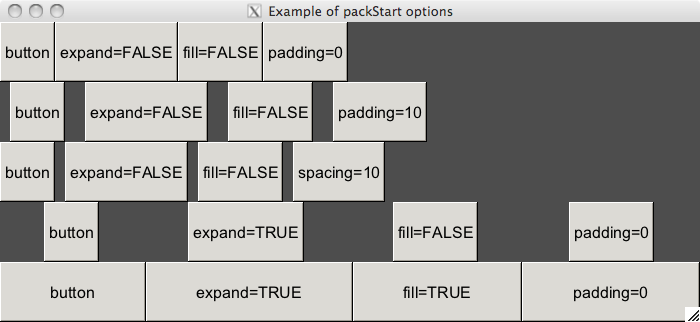
\includegraphics[width=.85\textwidth]{ex-RGtk2-pack-start}
  \caption{Examples of packing widgets into a box container. The top
    row shows no padding, whereas the 2nd and 3rd illustrate the
    difference between \code{padding} (an amount around each child)
    and \code{spacing} (an amount between each child). The last two
    rows show the effect of \code{fill} when \code{expand=TRUE}. This illustration
    follows one in orignial \GTK\/ tutorial.}
  \label{fig:RGtk2-pack-start}
\end{figure}




%% Resizing
\paragraph{Component size}
Each component has properties \code{width} and \code{height} to determine the size of the component when mapped. When these are both $-1$, the natural size of the widget will be used. To set the requested size of a component, the method \method{SetSizeRequest}{gtkWidget} is used to specify minimum values for the\code{width} and \code{height} of the widget. The methods help page warns that it is impossible to adequately hardcode a size that will always be correct.

When a parent container is resized, it queries its children for their
preferred size (\method{GetSizeRequest}{gtkWidget}), If these children
have children, they then are asked, etc. This size
information is then passed back to the top-level component. It resizes
itself, then passes on the available space to its children to resize
themselves, etc. After resizing the \method{GetAllocation}{gtkWidget}
method returns the new width and height, as components in a list.
The space allocated to a cell, may be more than the space requested by
the widget. In this case, the \argument{expand}{gtkBoxPackStart} and
\argument{fill}{gtkBoxPackStart} arguments for the \code{Pack} methods
are important. If \code{expand=TRUE} is given, then the cell will
expand to fill the extra space. Furthermore, if also \code{fill=TRUE} then
the widget will expand to fill the space allocated to the cell.
Figure~\ref{fig:RGtk2-pack-start} illustrates.


%% alignment of widgets within cells
\paragraph{Alignment}
Widgets inherit the properties \code{xalign} and \code{yalign} from
the \class{GtkMisc} class. These properties are used to specify how
the widget is aligned within the cells when the widget size request is
less than that allocated to the cell. These properties take values between $0$ and
$1$, with $0$ being left and top. Their defaults are $0.5$, for centered alignment.


% \begin{figure}
%   \centering
%   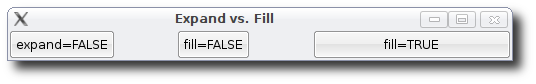
\includegraphics[width=.6\textwidth]{RGtk2-GtkBox-expand-fill}
%   \caption{Illustration of \code{expand} and \code{fill} arguments for
%     a \code{GtkBox} container. The \code{expand} argument causes the
%     cell to expand to fill all possible space. The \code{fill}
%     argument then indicates if the widget should then stretch to fill
%     the space allocated to its cell.}
%   \label{fig:RGtk2:GtkBox-expand-fill}
% \end{figure}






\section{Buttons}
\label{sec:RGtk2:gtkButton}

A basic button is constructed using \constructor{gtkButton}. This is a
convenience wrapper for several constructors. With no argument, it
returns a simple button. When the first argument, \argument{label}{gtkButton}, is
used it returns a button with a label, calling
\function{gtkButtonNewWithLabel}. The \argument{stock.id}{gtkButton} argument
calls \function{gtkButtonNewFromStock}.  Buttons in \GTK\/ are
actually containers (of class \class{GtkBin}), By default, they have a
\code{label} and \code{image} property. The image is specified using a
stock id. The available stock icons are listed by
\function{gtkStockListIds}. Finally, if a mnemonic is desired, for the
button, the constructor \constructor{gtkButtonNewWithMnemonic} can be
used. Mnemonics are specified by prefixing the character with an
underscore, as illustrated in this example.

\begin{example}{Button constructors}{eg:RGtk2:button-constructors}
\begin{Schunk}
\begin{Sinput}
 w <- gtkWindow(show=FALSE)
 w$setTitle("Various buttons")
 w$setDefaultSize(400, 25)
 g <- gtkHBox(homogeneous=FALSE, spacing=5)
 w$add(g)
 b <- gtkButtonNew(); 
 b$setLabel("long way")
 g$packStart(b)
 g$packStart(gtkButton(label="label only") )
 g$packStart(gtkButton(stock.id="gtk-ok") )
 g$packStart(gtkButtonNewWithMnemonic("_Mnemonic") ) # Alt-m to "click"
 w$show()
\end{Sinput}
\end{Schunk}
\end{example}

\begin{figure}
  \centering
  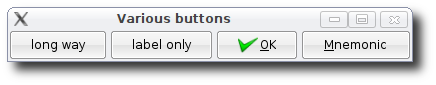
\includegraphics[width=.8\textwidth]{RGtk2-various-button}
  \caption{Various buttons}
  \label{fig:RGtk2:various-buttons}
\end{figure}

Buttons are essentially containers with a decoration to give them a
button like appearance. The relief style of the button can be changed
so that the button is drawn like a label. The method
\method{SetRelief}{gtkButton} is used, with the available styles
found in the \code{GtkReliefStyle} enumeration.

A button, can be drawn with extra space all around it. The
\code{border-width} property, with default of 0, specifies this space.
One can use the method \method{SetBorderWidth}{gtkContainer} to make
a change.


%% signals
\paragraph{Signals}
The \signal{clicked} signal is emitted when the button is
clicked on with the mouse or when the button has focus and the
\kbd{enter} key is pressed. A callback can listen for this event, to
initiate an action.  If one wishes to filter out the mouse
button that was pressed on the button, the \signal{button-press-event} signal
is also emitted. Since this is a window manager event, the second
argument to the callback is an event which contains the button
information. This can be retrieved using the event's
\method{getButton}{gtkEventButton} method. However, the
\signal{button-press-event} signal is not emitted when the keyboard initiates
the action.

%% Buttons initiate actions
If the action a button is to initiate is the default action for the
window it can be set so that it is activated when the user presses
\kbd{enter} while the parent window has the focus. To implement this,
the property \code{can-default} must be \code{TRUE} and the widget
method \method{grabDefault}{gtkWidget} must be called. (This is not
specific to buttons, but any widget that can be activatable.)


As buttons are intended to call an action immediately after being
clicked, it is customary to make them not sensitive to user input when
the action is not possible. The \method{SetSensitive}{gtkWidget}
method can adjust this for the button, as with other widgets.


If the action that a button initiates is to be represented elsewhere
in the GUI, say a menu bar, then a \code{GtkAction} object may be
appropriate. Action objects are covered in
Section~\ref{sec:RGtk2:UIManager}.


\begin{example}{Callback example for \code{gtkButton}}{eg:RGtk2:gtkButton-callback}

\begin{Schunk}
\begin{Sinput}
 w <- gtkWindow(); b <- gtkButton("click me");
 w$add(b)
 ID <- gSignalConnect(b,"button-press-event",   # just mouse click
                      f = function(w,e,data) {
                        print(e$getButton())    # which button
                        return(FALSE)           # propogate
                      })
 ID <- gSignalConnect(b,"clicked",              # click or keyboard
                      f = function(w,...) {
                        print("clicked")
                      })
\end{Sinput}
\end{Schunk}
\end{example}


\begin{example}{Spacing between buttons}{eg:RGtk2:mac-buttons}
This example shows how to pack buttons into a box so that the spacing
between the similar buttons is 12 pixels, but between potentially
dangerous buttons is 24 pixels, as per the Mac human interface
guidelines.
\GTK\/ provides the constructor \constructor{gtkHButtonBox} for
holding buttons, which provides a means to apply consistent styles,
but the default styles do not allow such spacing as desired. (Had all
we wanted was to right align the buttons, then that style is certainly
supported.) As such, we will illustrate how this can be done through a
combination of \code{spacing} arguments.
We assume that our parent container, \code{g}, is a
horizontal box container.


\begin{figure}
  \centering
  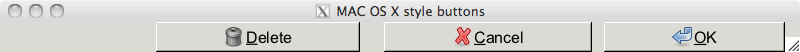
\includegraphics[width=.85\textwidth]{ex-RGtk2-mac-buttons}
  \caption{Example using stock buttons with extra spacing added between the \code{delete} and \code{cancel} buttons.}
  \label{fig:ex-RGtk2-mac-buttons}
\end{figure}

We include standard buttons, so use the stock names and icons.
\begin{Schunk}
\begin{Sinput}
 cancel <- gtkButton(stock.id="gtk-cancel")
 ok <- gtkButton(stock.id="gtk-ok")
 delete <- gtkButton(stock.id="gtk-delete")
\end{Sinput}
\end{Schunk}

We will right align our buttons, so use the parent container's
\code{PackEnd} method. The \code{ok} button has no padding, the
12-pixel gap between it and the \code{cancel} button is ensured by  the
\code{padding} argument when the \code{cancel} button is
added. Treating the \code{delete} button as potentially irreversible,
we aim to have 24 pixels of seperation between it and the
\code{cancel} button. This is given by adding 12 pixels of padding
when this button is packed in, giving 24 in total. The blank label is
there to fill out space if the parent container expands.
\begin{Schunk}
\begin{Sinput}
 g$packEnd(ok, padding=0)
 g$packEnd(cancel, padding=12)
 g$packEnd(delete, padding=12)
 g$packEnd(gtkLabel(""), expand=TRUE, fill=TRUE)
\end{Sinput}
\end{Schunk}
We make \code{ok} the default button, so have it grab the focus and
add a simple callback when the button is either clicked or the
\kbd{enter} key is pressed when the button has the focus.
\begin{Schunk}
\begin{Sinput}
 ok$grabFocus()
 QT <- gSignalConnect(ok, "clicked", function(...) print("ok"))
\end{Sinput}
\end{Schunk}






\end{example}

\section{Labels}
\label{sec:RGtk2:gtkLabel}

Labels are created by the \constructor{gtkLabel} constructor. Its main
argument is \argument{str}{gtkLabel} to specify the button text,
through its \code{label} property. This text can be set with either
\method{SetLabel}{gtkLabel} or \method{SetText}{gtkLabel} and
retrieved with either \method{GetLabel}{gtkLabel} or \method{GetText}{gtkLabel}.
The difference being the former can respect formatting marks. 

The text can include line breaks, specified with ``\code{\backslashn}.''
Further formatting is available. Wrapping of long labels can be
specified using a logical value with the method
\method{SetLineWrap}{gtkLabel}. The line width can be specified in
terms of the number of characters thorugh
\method{SetWidthChars}{gtkLabel} or by setting the size request for
the label. This is not determined by the size of the parent
window. Long labels can also have ellipsis inserted into them to
shorten when there is not enough space. By default this is turned
off. The variable \code{PangoEllipsizeMode} contains the constants,
and the method \method{SetEllipsize}{gktkLabel} is used to set this.
The property \code{justify}, with values taken from
\code{GtkJustification}, controls the justification.


\GTK\/ allows markup of text elements using the Pango text attribute
markup language. The method \method{SetMarkup}{gtkLabel} is used to
specify the text in the format, which is similar to a basic subset of
HTML. Text is marked using tags to indicate the style. Some convenient
tags are \code{<b>} for bold, \code{<i>} for italics, \code{<ul>} for
underline, and \code{<tt>} for monospace text. More complicated markup
involves the \code{<span>} tag markup, such as \code{<span color='red'>some text</span>}. The text can may need to be escaped first, so that designated entities replace reserved characters.



By default, text in a label can not be copied and pasted into another
widget or application. To allow this, the \code{selectable} property
can be set to \code{TRUE} with \method{SetSelectable}{gtkLabel}.
Labels can hold mnemonics for other widgets. The constructor is
\code{gtkLabelNewWithMnemonic}. The label needs to idenfy the widget
it is holding a mnemonic for, this is done with the
\method{SetMnemonicWidget}{gtkLabel} method.

\begin{example}{Label formatting}{eg:RGtk2:label-formatting}
  This examples shows various label formatting techniques~(Figure~\ref{})>
  
\begin{figure}
  \centering
  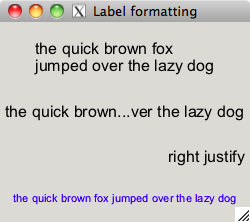
\includegraphics[width=.6\textwidth]{fig-RGtk2-labels}
  \caption{Various formatting for a label: wrapping, alignment, ellipsizing, PANGO markup}
  \label{fig:RGtk2:label-formatting}
\end{figure}
 
\begin{Schunk}
\begin{Sinput}
 w <- gtkWindow(); w$setTitle("Label formatting")
 w$setSizeRequest(250,100)               # narrow
 g <- gtkVBox(spacing=2); g$setBorderWidth(5); w$add(g)
 string = "the quick brown fox jumped over the lazy dog"
 ## wrap by setting number of characters
 basicLabel <- gtkLabel(string)
 basicLabel$setLineWrap(TRUE); 
 basicLabel$setWidthChars(35)            # specify number of characters
 ## Set ellipsis to shorten long text
 ellipsized <- gtkLabel(string)
 ellipsized$setEllipsize(PangoEllipsizeMode["middle"])
 ## Right justify text
 ## use xalign property for label in cell
 rightJustified <- gtkLabel("right justify"); 
 rightJustified$setJustify(GtkJustification["right"])
 rightJustified['xalign'] <- 1
 ## PANGO markup
 pangoLabel <- gtkLabel(); 
 pangoLabel$setMarkup(paste("<span foreground='blue' size='x-small'>",
                            string,"</span>"));
 QT <- sapply(list(basicLabel, ellipsized, rightJustified, pangoLabel),
              function(i) g$packStart(i, expand=TRUE, fill=TRUE ))
 w$showAll()
\end{Sinput}
\end{Schunk}
\end{example}

%% signals
\paragraph{Signals}
Unlike buttons, labels do not emit any signals. Labels are intended to
hold static text. However, if one wishes to define callbacks to react
to events, then the label can be placed within an instance of
\constructor{gtkEventBox}. This creates a non-visible parent window
for the label that does signal
events. Example~\ref{eg:RGtk2:editable-label} will illustrate the use
of an event box.  Alternatively, one could use an instance of
\code{gtkButton} with its \code{relief} property assigned to
\code{GtkReliefStyle['none']}.


\subsection{Link Buttons}
\label{sec:link-buttons}

A link button is a special label which shows an underlined link, such
as is done by a web browser. (Newer versions of \GTK\/ allow the label
of a button to contain HTML links.) The \code{uri} is specified to the
\constructor{gtkLinkButton} constructor with an optional
\argument{label}{gtkLinkButton} argument. If none is specified, the
\code{uri} is used to provide the value. This \code{uri} is stored in
the \code{uri} property and the label in the \code{label} value. These
may be adjusted later.

As the link button inherits from the \class{gtkButton} class, the
\code{clicked} signal is emitted when a user clicks a mouse on the link.

\begin{example}{Basic link button usage}{eg:RGtk2:link-button}
\begin{Schunk}
\begin{Sinput}
 w <- gtkWindow()
 g <- gtkVBox(); w$add(g)
 lb <- gtkLinkButton(uri="http://www.r-project.org")
 lb1<- gtkLinkButton(uri="http://www.r-project.org", label="R Home")
 g$packStart(lb)
 g$packStart(lb1)
 f <- function(w,...) browseURL(w['uri'])
 ID <- gSignalConnect(lb,  "clicked", f = f)
 ID <- gSignalConnect(lb1, "clicked", f = f)
\end{Sinput}
\end{Schunk}
\end{example}


\section{Images}
\label{sec:RGtk2:images}

Images in \pkg{RGtk2} are constructed with
\constructor{gtkImage}. This is a front end for several constructors:
\constructor{gtkImageNewFromIconSet},
\constructor{gtkImageNewFromPixmap},
\constructor{gtkImageNewFromImage}, \constructor{gtkImageNewFromFile},
\constructor{gtkImageNewFromPixbuf},
\constructor{gtkImageNewFromStock},
\constructor{gtkImageNewFromAnimation}. We only discuss loading an
image from a file, and so use the \constructor{gtkImageNewFromFile}
constructor. To add an image after construction of the main widget,
the \constructor{gtkImageNew} constructor can be used along with
methods such as \method{SetFromFile}{gtkImage}.

The image widget, like the label widget, does not have a parent
GdkWindow, which means it does not receive window events. As with the
label widget, the image widget can be placed inside a
\constructor{gtkEventBox} container if one wishes to connect to such
events.



\begin{example}{Using a pixbuf to present graphs}{ex:RGtk2:pixbuf}

  This example shows how to use a \constructor{gtkImage} object to
  embed a graphic within \pkg{RGtk2}, as an alternative to using the
  \pkg{cairoDevice} package. The basic idea is to use the
  \function{Cairo} device to create a file containing the graphic, and
  then use \constructor{gtkImageNewFromFile} to construct a widget to
  show the graphic.

  We begin by creating a window of a certain size.
\begin{Schunk}
\begin{Sinput}
 w <- gtkWindow(show=FALSE); w$setTitle("Graphic window");
 w$setSizeRequest(400,400)
 g <- gtkHBox(); w$add(g)
 w$showAll()
\end{Sinput}
\end{Schunk}


The size of the image is retrieved from the size allocated to the box
\code{g}. This allows the window to be resized prior to drawing the
graphic. Unllke an interactive device, after drawing, this graphic
does not resize itself when the window resizes.

\begin{Schunk}
\begin{Sinput}
 theSize <- g$getAllocation()
 width <- theSize$width; height <- theSize$height
\end{Sinput}
\end{Schunk}

Now we draw a basic  graphic as a png file (\code{Cairo}'s default) stored in a temporary file.
\begin{Schunk}
\begin{Sinput}
 require(Cairo)
 filename <- tempfile()
 Cairo(file = filename, width = width, height = height)
 hist(rnorm(100))
 QT <- dev.off()
\end{Sinput}
\end{Schunk}

The constructor may be called as \command{gtkImage(filename=filename)}
or as follows:
\begin{Schunk}
\begin{Sinput}
 image <- gtkImageNewFromFile(filename)
 g$packStart(image, expand=TRUE, fill = TRUE)
 unlink(filename)                        # tidy up
\end{Sinput}
\end{Schunk}

\end{example}


\section{Stock icons}
\label{sec:RGtk2:stock-icons}

\GTK\/ comes with several ``stock'' icons. These are used by the
\constructor{gtkButton} constructor when its \code{stock.id} argument
is specified, and will be used for menubars, and toolbars. The size of
the icon used is one of the values returned by \code{GtkIconSize}.

As mentioned previously, the full list of stock icons are returned in
a list by \function{gtkStockListIds}. The first $4$ are:
\begin{Schunk}
\begin{Sinput}
 head(unlist(gtkStockListIds()), n=4)   
\end{Sinput}
\begin{Soutput}
[1] "gtk-zoom-out" "gtk-zoom-in"  "gtk-zoom-fit" "gtk-zoom-100"
\end{Soutput}
\end{Schunk}

To load a stock icon into an image widget, the
\constructor{gtkImageNewFromStock} can be used. The
\argument{stock.id}{gtkImageNewFromStock} contains the icon name and
\argument{size}{gtkImageNewFromStock} the size. 

The example below, we use the method \method{RenderIcon}{gtkWidget} to
return a pixbuf containing the icon that can be used with the
constructor \constructor{gtkImageNewFromPixbuf} to display the
icon. Here the stock id and size are specified to the
\method{RenderIcon}{gtkWidget} method.



\begin{example}{\constructor{gtkButtonNewFromStock} -- the hard way}{ex:RGtk2:stock-icon}
The following example, shows how to do the work of
\constructor{gtkButtonNewFromStock} by hand using an image and label together.
\begin{Schunk}
\begin{Sinput}
 b <- gtkButton()
 g <- gtkHBox()
 pbuf <- b$renderIcon("gtk-ok", size=GtkIconSize["button"]) 
 i <- gtkImageNewFromPixbuf(pbuf)
 i['xalign'] <- 1; i['xpad'] <- 5        # right align with padding
 g$packStart(i, expand=FALSE)
 l <- gtkLabel(gettext("ok")); 
 l['xalign'] <- 0 # left align
 g$packStart(l, expand=TRUE, fill=TRUE)
 b$add(g)
 ## show it
 w <- gtkWindow(); w$add(b)
\end{Sinput}
\end{Schunk}
\end{example}

%% Only for the package
%% Adding icons to stock
\begin{example}{Adding to the stock icons}{ex:RGtk2:add-stock-icons}
This example shows, without much explanation the steps to add images
to the list of stock icons. To generate some sample icons, we use
those provided by objects in the \pkg{ggplot2} package.




First we create the icons using the fact that the objects have a function \code{icon} to draw an image.
\begin{Schunk}
\begin{Sinput}
 require(ggplot2)
 require(Cairo)
 iconNames <- c("GeomBar","GeomHistogram")   # 2 of many ggplot functions
 icon.size <- 16
 iconDir <- tempdir()
 fileNames <- sapply(iconNames, function(name) {
   nm <- paste(iconDir, "/", name, ".png", sep="", collapse="")
   Cairo(file=nm, width=icon.size, height=icon.size, type="png")
   val <- try(get(name))
   grid.newpage()
   try(grid.draw(val$icon()), silent=TRUE)
   dev.off()
   nm
 })
\end{Sinput}
\end{Schunk}
The following function works through the steps to add a new icon. The
basic ideas are sketched out in the API for \code{GtkIconsSet}.
\begin{Schunk}
\begin{Sinput}
 addToStockIcons <- function(iconNames, fileNames, stock.prefix="new") {
   iconfactory <- gtkIconFactoryNew()
   
   for(i in seq_along(iconNames)) {
     
     iconsource = gtkIconSourceNew()
     iconsource$setFilename(fileNames[i])
     
     iconset = gtkIconSetNew()
     iconset$addSource(iconsource)
     
     stockName = paste(stock.prefix, "-", iconNames[i], sep="")
     iconfactory$add(stockName, iconset)
     
     items = list(test=list(stockName, iconNames[i],"","",""))
     gtkStockAdd(items)
   }
   iconfactory$AddDefault()
   invisible(TRUE)
 }
\end{Sinput}
\end{Schunk}
We call this function and then check that the values are added:
\begin{Schunk}
\begin{Sinput}
 addToStockIcons(iconNames, fileNames)
 nms <- gtkStockListIds()
 unlist(nms[grep("^new", nms)])
\end{Sinput}
\begin{Soutput}
[1] "new-GeomHistogram" "new-GeomBar"      
\end{Soutput}
\end{Schunk}

\end{example}



%% Alertpanel application
\begin{example}{An alert panel}{eg:RGtk2:alert-panel}

\begin{figure}
  \centering
  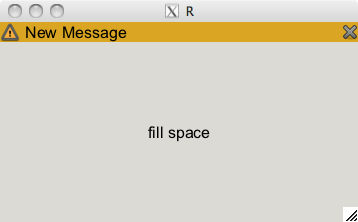
\includegraphics[width=.45\textwidth]{ex-RGtk2-alert-panel}
  \caption{The alert panel showing a message.}
  \label{fig:RGtk2-alert-panel}
\end{figure}

This example puts together images, buttons, labels and box containers
to create an alert panel, or information bar. This is an area that
seems to drop down from the menu bar to give users feedback about an
action that is less disruptive than a modal dialog. A similar widget
is used in the Firefox browser with its popup blocker. Although, as of version
2.18, a similar feature is available in \GTK\/ through the
\code{GtkInfoBar} widget, this example is given, as it shows how
several useful things in \GTK\/ can be combined to customize the user
experience.

This constructor for the widget specifies some properties and returns
an environment to store these properties, as our function calls will
need to update these properties and have be persistent.
\begin{Schunk}
\begin{Sinput}
 newAlertPanel <- function(wrap=35,
                           icon="gtk-dialog-warning",
                           message="",
                           panel.color="goldenrod",
                           evb=NULL,
                           image=NULL,
                           label=NULL # info
                     ) {
   x <- c("wrap","icon","message","panel.color","evb","image","label")
   e <- new.env()
   sapply(x, function(i) assign(i, envir=e, get(i)))
   return(e)
 }
\end{Sinput}
\end{Schunk}

An alert panel needs just a few methods: one to create the widget, one
to show the widget and one to hide the widget. We create a function
\code{getAlertPanelBlock} to return a component that can be added to a
container. An event box is used so that we can color the background,
as this isn't possible for a box container due to its lack of a gdk
window.  To this event box we add a box container that will hold an
icon indicating this is an alert, a label for the message, and another
icon to indicate to the user how to close the alert. Since we wish to
receive mouse clicks on close icon, we place this inside another event
box. To this, we bind a callback to the \signal{button-press-event} signal.
\begin{Schunk}
\begin{Sinput}
 getAlertPanelBlock <- function(obj) {
 
   obj$evb <- gtkEventBox(show=FALSE)
   obj$evb$ModifyBg(state="normal",color=obj$panel.color)
 
   g <- gtkHBox(homogeneous=FALSE, spacing=5)
   obj$evb$add(g)
 
   obj$image <- gtkImageNewFromStock(obj$icon, size="button")
   obj$image['yalign'] <- .5
   g$packStart(obj$image, expand=FALSE)
 
   obj$label <- gtkLabel(obj$message)
   obj$label['xalign'] <- 0; obj$label['yalign'] <- .5
   obj$label$setLineWrap(TRUE)
   obj$label$setWidthChars(obj$wrap)
   g$packStart(obj$label, expand=TRUE, fill=TRUE)
 
   xbutton <- gtkEventBox()
   xbutton$modifyBg(state="normal", color=obj$panel.color) 
   xbutton$add(gtkImageNewFromStock("gtk-close", size="menu"))
   g$packEnd(xbutton, expand=FALSE, fill=FALSE)
   xbuttonCallback <- function(data, widget,...) {
     hideAlertPanel(data)
     return(FALSE)
   }
 
   ## close on button press and event box click
   sapply(list(xbutton, obj$evb), function(i) {
     gSignalConnect(i, "button-press-event",
                    f=xbuttonCallback,
                    data=obj, user.data.first=TRUE)
     })
   return(obj$evb)
 }
\end{Sinput}
\end{Schunk}

The \code{showAlertPanel} function updates the message and then calls
the \method{Show}{gtkWidget} method of the event box.

\begin{Schunk}
\begin{Sinput}
 showAlertPanel <- function(obj) {
   obj$label$setText(obj$message)
   obj$evb$show()
 }
\end{Sinput}
\end{Schunk}

Our \code{hideAlertPanel} function simply calls the \method{hide}{gtkWidget}
method the event box.
\begin{Schunk}
\begin{Sinput}
 hideAlertPanel <- function(obj) obj$evb$hide()
\end{Sinput}
\end{Schunk}

To test it out, we create a simple GUI
\begin{Schunk}
\begin{Sinput}
 w <- gtkWindow()
 g <- gtkVBox(); w$add(g)
 ap <- newAlertPanel()
 g$packStart(getAlertPanelBlock(ap), expand=FALSE)
 g$packStart(gtkLabel("fill space"), expand=TRUE, fill=TRUE)
 ap$message <- "New Message"             # add message
 showAlertPanel(ap)
\end{Sinput}
\end{Schunk}

To improve this, one could also add a time to close the panel after some delay. The
\function{gTimeoutAdd} function is used to specify a function to call
periodically until the function returns \code{FALSE}.

\end{example}

\section{Text entry}
\label{sec:RGtk2:gtkEntry}

A one-line text entry widget is constructed by
\function{gtkEntry}. An  argument \argument{max}{gtkEntry} specifies
the maximum number of characters if positive, but this calls a
deprecated function, so this restriction should be set using the
method \method{SetMaxLength}{gtkEntry}.

The \code{text} property stores the text. This can be set with the
method \method{SetText}{gtkEntry} and retrieved with
\method{GetText}{gtkEntry}. The method
\method{InsertText}{gtkEditable} is used to insert text.  Its argument
\argument{new.text}{gtkEditableInsertText} contains the text and
\argument{position}{gtkEditableInsertText} specifies the position of
the text to be added. The return value is a list with components
\code{position} indicating the position \textit{after} the new
text. The \method{DeleteText}{gtkEditable} method can be used to
delete text. This takes two integers indicating the start and finish
location of the text.

\begin{example}{Insert and Delete text}{eg:RGtk2:insert-delete-text}
The example will show how to add then delete text.  
\begin{Schunk}
\begin{Sinput}
 e <- gtkEntry()
 e$setText("Where did that guy go?")
 add.pos <- regexpr("guy", e['text']) - 1 # before "guy"
 ret <- e$insertText("@$#%! ", position = add.pos)
 e$getText()                             # or e['text']
\end{Sinput}
\begin{Soutput}
[1] "Where did that @$#%! guy go?"
\end{Soutput}
\begin{Sinput}
 e$deleteText(start = add.pos, end= ret$position)
 e$getText()
\end{Sinput}
\begin{Soutput}
[1] "Where did that guy go?"
\end{Soutput}
\end{Schunk}
\end{example}

%% signals
The \class{GtkEntry} class adds three signals \signal{changed} when
text is changed, \signal{delete-text} for delete events, and
\signal{insert-text} for insert events. The \signal{changed} signal will
be emitted each time there is a keypress, while the widget has
focus. When the \kbd{enter} key is pressed the \signal{activate} signal
is also emitted. 

%% skipped
% \begin{example}{Editable label}{eg:RGtk2:editable-label}
%   \SweaveInput{ex-RGtk2-editable-label}
% \end{example}


\section{Check button}
\label{sec:RGtk2:gtkCheckbox}

A check button widget is constructed by \function{gtkCheckButton}. The
optional argument \argument{label}{gtkCheckButton} places a label next
to the button. The label can have a mnemonic, but then the constructor
is  \constructor{gtkCheckButtonewWithMnemonic}.

The \code{label} property stores the label. This can be set or
retrieved with the methods \method{SetLabel}{gtkButton} and
\method{GetLabel}{gtkButton}. 

A check button's state is stored as a logical variable in its
\code{active} property. It can be set or retrieved with the methods
\method{SetActive}{gtkToggleButton} and
\method{GetActive}{gtkToggleButton}. 

When the state is changed the \signal{toggle} signal is emitted.


\subsection{Toggle buttons}
\label{sec:ToggleButtons}

A toggle button, is a useful way to set configuration values in an
obvious way to the user.  A toggle button has a depressed look when in
an active state. The \constructor{gtkToggleButton} constructor is
used to create toggle buttons. The \argument{label}{gtkToggleButton}
argument sets the \code{label} property. This can also be set or
retrieved with the methods \method{SetLabel}{gtkButton} and
\method{GetLabel}{gtkButton}.

%% active property
The \code{active} property is \code{TRUE} when the button is
depressed, and \code{FALSE} otherwise. This can be queried with the
\method{GetActive}{gtkToggleButton} method.

%% signal clicked
As with other buttons, the \code{clicked} signal is emitted when the user
clicks on the button.


\section{Radio groups}
\label{sec:RGtk2:gtkRadioButton}

The \function{gtkRadioButton} constructor is used to create linked
radio buttons.  The argument \argument{group}{gtkRadioButton} if
missing or \code{NULL} will create a new radio button group. If
specified as a list of radio buttons, will create a new button for the
group.  The constructor returns a single radio button widget.  The
labels for each individual button are determined by their \code{label}
property, This can be set at construction time through the
\argument{label}{gtkRadioButton}, or can be modified through the
\method{SetLabel}{gtkButton} method.

%% active
Each radio button in the group has its \code{active} property either
\code{TRUE} or \code{FALSE}, although only one can be \code{TRUE} at a
time. The methods \method{GetActive}{gtkToggleButton} and \method{SetActive}{gtkToggleButton} may be used to manipulate the state of an individual button. To determine which button is active, they can be queried
individually. The same property can be set to make a given button
active.  

%% --- toggled signal ---
When the state of a radio button is changed, it emits the
\signal{toggled} signal. To assign a callback to this event, each
button in the group must register a callback for this signal The
\code{active} property can be queried to decide if the toggle is from
being selected, or deselected.


\begin{example}{Radio group construction}{eg:RGtk2:radio-buttons}
Creating a new radio button group follows this pattern:
\begin{Schunk}
\begin{Sinput}
 vals <- c("two.sided", "less", "greater")
 l <- list()                                 # list for group
 l[[vals[1]]] <- gtkRadioButton(label=vals[1]) # group = NULL
 for(i in vals[-1]) 
   l[[i]] <- gtkRadioButton(l, label=i)  # group is a list
\end{Sinput}
\end{Schunk}
Each button needs to be managed. Here we illustrate a simple GUI doing so.
\begin{Schunk}
\begin{Sinput}
 w <- gtkWindow(); w$setTitle("Radio group example")
 g <- gtkVBox(FALSE, 5); w$add(g)
 QT <- sapply(l, function(i) g$packStart(i))
\end{Sinput}
\end{Schunk}
We can set and query which button is active, as follows:
\begin{Schunk}
\begin{Sinput}
 l[[3]]$setActive(TRUE)           
 sapply(l, function(i) i$getActive()) 
\end{Sinput}
\begin{Soutput}
two.sided      less   greater 
    FALSE     FALSE      TRUE 
\end{Soutput}
\end{Schunk}
Here is how we might register a callback for the \code{toggled} signal.
\begin{Schunk}
\begin{Sinput}
 QT <- sapply(l, function(i) 
        gSignalConnect(i, "toggled",     # attach each to "toggled"
                       f = function(w, data) {
                         if(w$getActive()) # set before callback
                           cat("clicked", w$getLabel(),"\n")
                       }))
\end{Sinput}
\end{Schunk}
\end{example}

The \pkg{RGtk2} package coverts a list in \R\/ to the appropriate list
for \GTK. However, you may wish to refer to this list within a
callback, but only the current radio button is passed through. Rather
than passing the list through the \code{data} argument or using a
global, The \method{GetGroup}{gtkRadioButton} method can be used to
reference the buttons stored within a radio group. This method returns
a list containing the radio button. However, it is in the reverse
order of how they were added (newest first). (As GLib list uses
prepend to add elements, not append, as it is more efficient.)

\begin{example}{Radio group using \code{GetGroup}}{eg:gtk:radio-group-get-group}
  In this example below, we illustrate two things: using the
  \method{NewWithLabelFromWidget}{gtkRadioButton} method to add new
  buttons to the group and the \method{GetGroup}{gtkRadioButton}
  method to reference the buttons. The \function{rev} function is used
  to pack the widgets, to get them to display first to last.
\begin{Schunk}
\begin{Sinput}
 radiogp <- gtkRadioButton(label=vals[1])
 for(i in vals[-1])
   radiogp$newWithLabelFromWidget(i)
 w <- gtkWindow(); 
 w['title'] <- "Radio group example"
 g <- gtkVBox(); w$add(g)
 QT <- sapply(rev(radiogp$getGroup()),         # reverse list
              function(i) g$packStart(i))
\end{Sinput}
\end{Schunk}
\end{example}

\section{Combo boxes}
\label{sec:RGtk2:basic-combobox}

A basic combobox is constructed by
\constructor{gtkComboBoxNewText}. Later we will discuss more
complicated comboboxes, where a backend model is manipulated.
% Unlike
% others, as of writing, this widget must have its
% \method{Show}{gtkWidget} method called to be mapped.

For the basic combobox, items may be added to the combobox in a few
manners: to add to the end or beginning we have
\method{AppendText}{gtkComboBox} and
\method{PrependText}{gtkComboBox}; to insert within the list the
\method{InsertText}{gtkComboBox} method is used with the argument
\argument{position}{gtkComboBoxInsertText} specified in addition to
the argument \argument{text}{gtkComboBoxInsertText} to indicate the
index where the values should added. (The prepend method would be
index $0$, the append method would be with an index equal to the
number of existing items.)

The currently selected value is specified by index with the method
\method{SetActive}{gtkComboBox} and returned by
\method{GetActive}{gtkComboBox}. The index, as usual, is $0$-based, and in
this case uses a value of $-1$ to specify that no value is selected.
The \method{GetActiveText}{gtkComboBox} method can be used to retrieve the text shown by the basic combo box

It can be difficult to use a combobox when there are a large number of
selections. The \method{SetWrapWidth}{gtkComboBox} method allows the
user to specify the preferred number of columns to be used to display
the data.


%% signal
The main signal to connect to is \signal{changed} which is emitted
when the active item is changed either by the user or the programmer
through the \code{GetActive} method.

\begin{example}{Combo box}{eg:RGtk2:simple-combo-box}
A simple combobox may be produced as follows:
\begin{Schunk}
\begin{Sinput}
 vals <- c("two.sided", "less", "greater")
 cb <- gtkComboBoxNewText()
 for(i in vals) cb$appendText(i)
 cb$setActive(0)                         # first one
 ID <- gSignalConnect(cb, "changed",
                      f = function(w, ...) {
                        i <- w$getActive() + 1 # shift index
                        if(i == 0) 
                          cat("No value selected\n")
                        else
                          cat("Value is", w$getActiveText(), "\n")
                      })
\end{Sinput}
\end{Schunk}
A simple GUI is shown, the call to \code{ShowAll} is used here, as this
widget does not get mapped without its \code{Show} method being called.
\begin{Schunk}
\begin{Sinput}
 w <- gtkWindow(show=FALSE)
 w['title'] <- "Combobox example"
 w$add(cb)
 w$showAll()    # propogate down to cb
\end{Sinput}
\end{Schunk}
\end{example}




\subsection{Sliders}
\label{sec:RGtk2:sliders}

The slider widget and spinbutton widget allow selection from a
regulary spaced list of values. In \GTK\/ these values are stored in an
adjustment object, whose details are mostly hidden in normal use.

The slider widget in \GTK\/ may be oriented either horizontally or
vertically. The decision
is made through the choice of constructor: \constructor{gtkHScale} or
\constructor{gtkVScale}. For these widgets, the adjustment can be
specified -- if desired, or for convenience, will be created if the arguments
\argument{min}{gtkHScale}, \argument{max}{gtkHScale}, and
\argument{step}{gtkHScale} are given.  These arguments take  numeric
values. As the first argument (\argument{adjustment}{gtkHScale}) is
used to specify an adjustment,
these values are best specified by name. Alternatively, the
\constructor{gtkHScaleNewWithRange} constructor can be used with
positional arguments for \code{min}, \code{max} and \code{step}.


The methods \method{GetValue}{gtkRange} and
\method{SetValue}{gtkRange} can be used to return and set the value of
the widget. When assigning a value, values outside the bounds will be
set to the minimum or maximum value.

%% properties
A few properties can be used to adjust the appearance of the slider widget.
The \code{digits} property controls the number of digits after the
decimal point that are displayed.  The property \code{draw-value} can be
used to turn off the drawing of the selected value near the
slider. Finally, the property \code{value-pos} specifies where this
value will be drawn using values from \code{GtkPositionType}. The
default is \code{top}.

%% value-changed
Callbacks can be assigned to the \code{value-changed} signal, which is
emitted when the slider is moved.

\begin{example}{A slider controlling histogram bin selection}{ex:RGtk2:sliders}
  A simple mechanism to make a graph interactive, is to have the
  graph redraw whenever a slider has its value changed. The following
  shows how this can be achieved.
\begin{Schunk}
\begin{Sinput}
 library(lattice)
 w <- gtkWindow(); w$setTitle("Histogram bin selection")
 slider <- gtkHScaleNewWithRange(1, 100, 1) # min, max, step
 slider$setValue(10)                        # initial val.
 slider['value-pos'] <- "bottom"
 w$add(slider)
 f <- function(val) print(histogram(x, nint = val))
 ID <- gSignalConnect(slider,"value-changed",
                f = function(w, ...) {
                  val <- w$getValue()
                  f(val)
                })
 x <- rnorm(100)                         # the data
 f(slider$getValue())                    # initial graphic
\end{Sinput}
\end{Schunk}
\end{example}

\subsection{Spinbuttons}
\label{sec:RGtk2:spinboxes}

The spinbutton widget is very similar to the slider widget in \GTK. Spinbuttons are constructed with
\constructor{gtkSpinButton}. As with sliders, this constructor allows a
specification of the adjustment with an actual adjustment, or through
the arguments \argument{min}{gtkSpinButton}, \argument{max}{gtkSpinButton}, and
\argument{step}{gtkSpinButton}. 

As with sliders, the methods
\method{GetValue}{gtkSpinButton} and \method{SetValue}{gtkSpinButton}
are used to get and set the widgets value. The property
\code{snap-to-ticks} can be set to \code{TRUE} to force the new value
to be one of sequence of values in the adjustment. The \code{wrap}
property indicates if the widget will ``wrap'' around when at the
bounds of the adjustment.

Again, as with sliders, the \code{value-changed} signal is emitted when the
spin button is changed. 

\begin{example}{A range widget}{ex:RGtk2-range-widget}
This example shows how to make a range widget that combines both the slider and spinbutton to choose a single number. Such a widget is popular, as the slider is easy to make large changes and the spinbutton better at finer changes. In \GTK\/ we use the same adjustment, so changes to one widget propogate without effort to the other.

\begin{Schunk}
\begin{Sinput}
 ## make a range widget combining both a slider and spinbutton to choose a number
 library(RGtk2)
\end{Sinput}
\end{Schunk}

Were this written as a function, an \R\/ user might expect the
arguments to match those of \code{seq}/
\begin{Schunk}
\begin{Sinput}
 from <- 0; to <- 100; by <- 1
\end{Sinput}
\end{Schunk}

The slider is drawn without a value, so that the user sees only that
in the spinbutton. This spinbutton is created by specifying the
adjustement created when the slider widget is.
\begin{Schunk}
\begin{Sinput}
 slider <- gtkHScale(min=from, max=to, step=by)
 slider['draw-value'] <- FALSE
 adjustment <- slider$getAdjustment()
 spinbutton <- gtkSpinButton(adjustment=adjustment)
\end{Sinput}
\end{Schunk}
Our layout places the two widgets in a horizontal box container with
the slider set to expand on a resize, but not the spinbutton.
\begin{Schunk}
\begin{Sinput}
 g <- gtkHBox()
 g$packStart(slider, expand=TRUE, fill=TRUE, padding=5)
 g$packStart(spinbutton, expand=FALSE, padding=5)
\end{Sinput}
\end{Schunk}


\end{example}

\subsection{The cairoDevice package}
\label{sec:cairodevice-package}

The package \pkg{cairoDevice} describes itself as a ``Cairo-based
cross-platform antialiased graphics device driver.''  It can be
embedded in a \pkg{RGtk2} GUI as with any other widget. Its basic
usage involves a few steps. First a new drawing area is made with
\constructor{gtkDrawingArea}. This drawing area can be
used by various drawing functions, that we do not describe. (In fact,
arbitrary widgets, such as pixbufs, can be used here.) The
\pkg{cairoDevice} package provides the function
\function{asCairoDevice} to coerce the drawing area to a graphics
device. This function has standard argument
\argument{pointsize}{asCairoDevice} and for some underlying widgets
\argument{width}{asCairoDevice} and \argument{height}{asCairoDevice} arguments.

\section{Containers}
\label{sec:containers}


In addition to boxes, there are a number of useful containers detailed
next. 


\subsection{Framed containers}
\label{sec:RGtk2:gtkFrame}

The \function{gtkFrame} function constructs a container with a
decorative frame to set off the containers components. The optional
\argument{label}{gtkFrame} argument can be used to specify the
\code{label} property. This can be subsequently retrieved and set
using the \method{GetLabel}{gtkFrame} and \method{SetLabel}{gtkFrame}
methods. The label can be aligned using the
\method{SetLabelAlign}{gtkFrame} method. This has arguments
\code{xalign} and \code{yalign}, with values in $[0,1]$, to specify the position of the label
relative to the frame.

Frames have a decorative shadow whose type is stored in the
\code{shadow-type} property. This type is a value from \code{GtkShadowType}.

Frames inherit from \class{GtkBin}, which means they have only one
child component. The \method{Add}{gtkContainer} method is used to add
it.

\subsection{Expandable containers}
\label{sec:RGtk2:gtkExpander}

Although they are a little unresponsive due to eventloop issues, an
expandable container proves quite useful to manage screen space. Expandable containers are
constructed by \function{gtkExpander}. Use
\function{gtkExpanderNewWithMnemonic} if a mnemonic is desired. The
containers are drawn with a trigger button and optional label, which can be
clicked on to hide or show the containers child.

The label can be given as an optional argument to the constructor, or
assigned later with the \method{SetLabel}{gtkExpander} method, The label can use
Pango markup. This is indicated by setting the \code{use-markup}
property  through \method{SetUseMarkup}{gtkExpander}. 

The state of the widget is stored in the \code{expanded} property,
which can be accessed with \method{GetExpanded}{gtkExpander} and
\method{SetExpanded}{gtkExpander}. 

As with frames, expanders inherit from \class{GtkBin} as well. The
child component is added through the  \method{Add}{gtkContainer} method.

When the state changes, the \signal{activate} signal is emitted.



\section{Divided containers}
\label{sec:RGtk2:gtkPanedWindow}

The \constructor{gtkHPaned} and \constructor{gtkVPaned} create
containers with a ``gutter'' to allocate the space between its two
children. 
% An example is presented in Example \ref{eg:RGtk2:using-tree-content}. 
Like the \class{gtkBin} containers,
the two spaces allow only one child component. The two children may be
added two different ways. The methods \method{Add1}{gtkPaned} and
\method{Add2}{gtkPaned} simply add the child, whereas the methods
\method{Pack1}{gtkPaned} and \method{Pack2}{gtkPaned} have arguments
\argument{resize}{gtkPanedPack1} and \argument{shrink}{gtkPanedPack1}
which specify how the child will resize if the paned container is
resized. These two arguments take logical values.  After children are
added, they can be referenced from the container through its
\method{GetChild1}{gtkPaned} and \method{GetChild2}{gtkPaned} methods.

The position of the gutter can be set with the
\method{SetPosition}{gtkPaned} method. This is given in terms of
screen position. The
properties \code{min-position} and \code{max-position} can be used to
convert a percentage into a screen position.

The \signal{move-handle} signal is emitted when the gutter position is
changed. 



\section{Notebooks}
\label{sec:RGtk2:gtkNotebook}

The \constructor{gtkNotebook} constructor creates a notebook container. The
default position of the notebook tabs is on the top, starting on the
left. The property \code{tab-pos} property
(\method{SetTabPos}{gtkNotebook}) uses the \code{GtkPositionType}
values of \qcode{left}, \qcode{right}, \qcode{top}, or \qcode{bottom} to adjust this. The
property \code{scrollable} should be set to \code{TRUE} to have the
widget gracefully handle the case when there are more page tabs than
can be shown at once. If the same size tab for each page is desired,
the method \method{SetHomogeneousTabs}{gtkNotebook} can be called with
a value of \code{TRUE}. 


%% adding pages
\paragraph{Adding pages to a notebook}
New pages can be added to the notebook with the
\method{InsertPage}{gtkNotebook} method. Each page of a notebook holds
one child component. This is specified with the
\argument{child}{gtkNotebookInsertPage} argument. The tab label can be
specified with the \argument{tab.label}{gtkNotebookInsertPage}
argument, but can also be set later with
\method{SetTabLabel}{gtkNotebook} and retrieved with
\method{getTabLabel}{gtkNotebook}. The label is specified using a
widget, such as a \function{gtkLabel} instance, but this allows for
more complicated tabs, such as a box container with a close icon. The
\method{SetTabLabelText}{gtkNotebook} can be used if just a text label
is desired. To use this method, the child widget is needed, which can
be retrieved with the
\method{[[}{GObject}
%%]]
%%
method or the \method{GetNthPage}{gtkNotebook} method. Both are an
alternative to getting all the children returned as a list through
\method{GetChildren}{gtkContainer}. By default, the new page will be
at the last position (the same as
\method{AppendPage}{gtkNotebook}). This can be changed by supplying
the desired position to the argument
\argument{position}{gtkNotebookInsertPage} using $0$-based indexing.
The default value is $-1$, indictating the last page.


%% page motions: reordered, deleted
\paragraph{Rearranging pages}
Pages can be reordered using the \method{ReorderChild}{gtkNotebook}
method. The arguments are the \argument{child}{gtkNotebook} for the
child widget, and \argument{position}{gtkNotebook}, again 0-based with
$-1$ indicating appending at the end. Pages can be deleted using the
method \method{RemovePage}{gtkNotebook}. The
\argument{page.num}{gtkNotebookRemovePage} argument specifies the page
by its position. If the child is known, but not the number the method
\method{PageNum}{gtkNotebook} returns the page number. Its argument is \argument{child}{gtkNotebookPageNum}.

%% movement
The current page number is stored in the \code{page} property.
The number of pages can be found by inspecting the length of the
return value of \method{GetChildren}{gtkContainer}, but more directly
is done with the method \method{GetNPages}{gtkNotebook}. A given page
can be raised with the \method{SetCurrentPage}{gtkNotebook}
method. The argument \argument{page.num}{gtkNotebookSetCurrentPage}
specifies which page number to raise. If the child container should
not be hidden, or the page won't change. Incremental movements are
possible through the methods \method{NextPage}{gtkNotebook} and
\method{PrevPage}{gtkNotebook}. 

\paragraph{Signals}
The notebook widget emits various signals when its state is
changed. Among these: the signal \signal{focus-tab} is emitted when a tab receives the
focus, \signal{select-page} is similar and the \signal{switch-page} is
emitted when the current page is changed.

\begin{example}{Adding a page with a close button}{eg:RGtk2-notebook-close-icon}
A familiar element of notebook tabs from web browsing is a close button. The following
defines a new method \method{InsertPageWithCloseButton}{gtkNotebook}
that will use an ``x'' to indicate a close button. An icon would be
prettier, of course. The callback passes both the notebook and the
page through the \code{data} argument, so that the proper page can be
deleted. One caveat, the simpler command \command{nb\$getCurrentPage()}
will return the page of the focused tab prior to clicking the "x"
button, which may not be the correct page to close.

\begin{Schunk}
\begin{Sinput}
 gtkNotebookInsertPageWithCloseButton <- 
   function(object, child, label.text="", position=-1) {
     label <- gtkHBox()
     label$packStart(gtkLabel(label.text))
     label$packEnd(b <- gtkButton("x"))   # prettier with icon
     ID <- gSignalConnect(b,"clicked",
                    function(userData, b, ...) {
                      nb <- userData$nb 
                      page <- userData$page
                      nb$removePage(nb$pageNum(page))
                    },
                    data = list(nb=object, page=child),
                    user.data.first=TRUE)
     object$insertPage(child, label, position)
   }
\end{Sinput}
\end{Schunk}

We now show a simple usage of a notebook.
\begin{Schunk}
\begin{Sinput}
 w <- gtkWindow()
 nb <- gtkNotebook(); w$add(nb)
 nb$setScrollable(TRUE)
 QT <- nb$insertPageWithCloseButton(gtkButton("hello"), 
                                    label.text="page 1")
 QT <- nb$insertPageWithCloseButton(gtkButton("world"), 
                                    label.text="page 2")
\end{Sinput}
\end{Schunk}
  
\end{example}


\subsection{Scrollable windows}
\label{sec:RGtk2:scroll-windows}

Scrollbars allow components that are larger than the space allotted to
be interacted with, by allowing the user to ajdust the visible portion
of the component. Scrollbars in \GTK\/ use adjustments (like the
spin button widget) to control the $x$ and $y$ position of the
displayed portion of the component.

The convenience function \constructor{gtkScrolledWindow} creates a
window that allows the user to scroll around its  child component. By
default, the horizontal and vertical adjustments are generated,
although, if desired, these
may be specified by the programmer.

Like a top-level window, a scrolled window is a \class{GtkBin} object
and has only one immediate child component. If this child is a tree
view, text view (discussed in the following), icon view, layout or
viewport the \method{add}{gtkContainer} method is used. Otherwise, the
method \method{addWithViewport}{gtkScolledWindow} can be used to create an
intermediate viewport around the child.


The properties \code{hscrollbar-policy} and \code{vscrollbar-policy}
determine if the scrollbars are drawn. By default, they are always
drawn. The \code{GtkPolicyType} enumeration, allows a specification of
\qcode{automatic} so that the scrollbars are drawn if needed, i.e, the
child component requests more space than can be allotted. The
\method{setPolicy}{gtkScrolledWindow} method allows both to be set at
once, as in the following example.

\begin{example}{Scrolled window example}{eg:RGtk2:scrolled-window}
This example shows how a scrolled window can be used to display a long list of values. The tree view
widget can also do this, but here we can very easily customize the display of each value. In the example, we simply locates where a label is placed.


\begin{Schunk}
\begin{Sinput}
 g <- gtkVBox(spacing=0)
 QT <- sapply(state.name, function(i) {
   l <- gtkLabel(i)
   l['xalign'] <- 0; l['xpad'] <- 10
   g$packStart(l, expand=TRUE, fill=TRUE)
 })
\end{Sinput}
\end{Schunk}

The scrolled window has just two basic steps in its construction. Here
we specify never using a scrolled window for the vertical display.
\begin{Schunk}
\begin{Sinput}
 sw <- gtkScrolledWindow()
 sw$setPolicy("never","automatic")
 sw$addWithViewport(g)                   # just "Add" for text, tree, ...
\end{Sinput}
\end{Schunk}

\begin{Schunk}
\begin{Sinput}
 w <- gtkWindow(show=FALSE)
 w$setTitle("Scrolled window example")
 w$setSizeRequest(-1, 300)
 w$add(sw)
 w$show()
\end{Sinput}
\end{Schunk}
\end{example}

\section{Tabular layout}
\label{sec:RGtk2:gtkTable}

The \constructor{gtkTable} constructor produces a container for laying
out objects in a tabular format. The container sets aside cells in a
grid, and a child component may occupy one or more cells. The
\argument{homogeneous}{gtkTable} argument can be used to make all
cells homogeneous in size. Otherwise, each column and row can have a
different size. At the time of construction, the number rows and
columns for the table many be specified with the
\argument{rows}{gtkTable} and \argument{columns}{gtkTable}
arguments. After construction, the \method{Resize}{gtkTable} method
can be used to resize these values.

%% adding children
Child components are added to this container through the
\method{AttachDefaults}{gtkTable} method. Its first argument,
\argument{child}{gtkTableAttachDefaults}, is the child component. This
component can span more than one cell. To specify which cells, the
arguments \argument{left.attach}{gtkTableAttachDefaults} and
\argument{right.attach}{gtkTableAttachDefaults} specify the columns through
the column number to attach the left (or right) side of the child to, and 
\argument{top.attach}{gtkTableAttachDefaults} and
\argument{bottom.attach}{gtkTableAttachDefaults} to specify the rows. 

The \method{Attach}{gtkTable} method is similar, but allows the
programmer more control over the placement of the child
component. This method has the arguments
\argument{xoptions}{gtkTableAttach} and
\argument{yoptions}{gtkTableAttach} to specify how the widget responds
to resize events. These arguments use the values of
\code{GtkAttachOptions} to specify either \qcode{expand},
\qcode{shrink} and/or \qcode{fill}. Just \qcode{fill} will cause the
widget to remain the same size if the window is enlarged, the
\qcode{expand} and \qcode{fill} combination will cause the component
to fill the available space, and the \code{shrink} option instructs
the widget to shrink if the table is made smaller through
resizing. Finally, the \argument{xpadding}{gtkTableAttach} and
\argument{xpadding}{gtkTableAttach} arguments allow the specification
of padding around the cell in pixels.


Anchoring of widgets within a cell can be done by setting the
\code{xalign} and \code{yalign} properties of the child widgets. 

%% JV: this doesn't add enough it seems
% \begin{example}{Layout of calculator buttons}{eg-RGtk2-calculator-buttons}
%   \SweaveInput{ex-RGtk2-calculator-buttons.Rnw}
% \end{example}


\begin{example}{Dialog layout}{ex-RGtk2-dialog-layout}
This example shows how to layout some controls for a dialog with some
attention paid to how the widgets are aligned and how they respond to
resizing of the window.

\begin{figure}
  \centering
  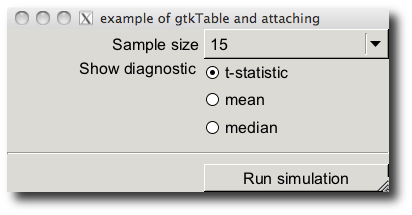
\includegraphics[width=.5\textwidth]{ex-RGtk2-dialog-layout}
  \caption{A basic dialog using a \code{gtkTable} container for layout.}
  \label{fig:RGtk2-dialog-layout}
\end{figure}


Our basic GUI is a table with 4 rows and 2 columns.
\begin{Schunk}
\begin{Sinput}
 w <- gtkWindow(show=FALSE)
 w$setTitle("example of gtkTable and attaching")
 tbl <- gtkTable(rows=4, columns=2, homogeneous=FALSE)
 w$add(tbl)
\end{Sinput}
\end{Schunk}

We define our widgets first then deal with their layout.
\begin{Schunk}
\begin{Sinput}
 l1 <- gtkLabel("Sample size")
 w1 <- gtkComboBoxNewText()
 QT <- sapply(c(5, 10, 15, 30), function(i) w1$appendText(i))
 l2 <- gtkLabel("Show diagnostic ")
 w2 <- gtkVBox()
 rb <- list()
 rb[["t"]] <- gtkRadioButton(label="t-statistic")
 for(i in c("mean","median")) rb[[i]] <- gtkRadioButton(rb, label=i)
 QT <- sapply(rb, function(i) w2$packStart(i))
 w3 <- gtkButton("Run simulation")
\end{Sinput}
\end{Schunk}

The basic \code{AttachDeafults} method will cause the widgets to
expand when resized, which we want to control here. As such we use
\code{Attach}. To get the control's label to center align yet still
have some breathing room we set its
\code{xalign} and  \code{xpad} properties.
For the combobox we avoid using \qcode{expand} as otherwise it resizes
to fill the space allocated to the cell in the \code{y} direction.
\begin{Schunk}
\begin{Sinput}
 tbl$attach(l1, left.attach=0,1, top.attach=0,1, yoptions="fill")
 l1["xalign"] <- 1; l1["xpad"] <- 5
 tbl$attach(w1, left.attach=1,2, top.attach=0,1, xoptions="fill", yoptions="fill")
\end{Sinput}
\end{Schunk}

We use \qcode{expand} here to attach the radio group, so that it
expands to fill the space. The label has its \code{yalign} proporty
set, so that it stays at the top of the cell, not the middle.
\begin{Schunk}
\begin{Sinput}
 tbl$attach(l2, left.attach=0,1, top.attach=1,2, yoptions="fill")
 l2["xalign"] <- 1; l2['yalign'] <- 0; l2["xpad"] <- 4
 tbl$attach(w2, left.attach=1,2, top.attach=1,2, xoptions=c("expand", "fill"))
\end{Sinput}
\end{Schunk}
A separator with a bit of padding provides a visual distinction
between the controls and the button to initiate an action.
\begin{Schunk}
\begin{Sinput}
 tbl$attach(gtkHSeparator(),left.attach=0,2, top.attach=2,3, ypadding=10, yoptions="fill")
 tbl$attach(w3, left.attach=1,2, top.attach=3,4, xoptions="fill", yoptions="fill")
\end{Sinput}
\end{Schunk}
Finally, we use the \code{ShowAll} method so that it propogates to the combobox.
\begin{Schunk}
\begin{Sinput}
 w$showAll()                             # propogate to combo
\end{Sinput}
\end{Schunk}
\end{example}



%% JV: this is in need of rewriting
\section{Drag and drop}
\label{sec:RGtk2:dnd}

%% ------------ Drag and Drop

\GTK\/ has mechanisms to provide drag and drop features to
widgets. Only widgets which can receive signals will work for drag and
drop, so to drag or drop on a label an event box must be used. To
setup drag and drop actions requires setting a widget to be a source
for a drag request, and setting a widget to be a target for a drop
action. We illustrate how to set up the dragging of a text value from
one widget to another. Much more complicated examples are possible,
but we do not pursue it here.

When a drag and drop is initiated, different types of data may be
transferred. \GTK\/ allows the user to specify a target type. Below,
we define target types for text, pixmap and arbitrary objects.

\begin{Schunk}
\begin{Sinput}
 ## info arguments -- application assigned
 TARGET.TYPE.TEXT   = 80                 
 TARGET.TYPE.PIXMAP = 81                  
 TARGET.TYPE.OBJECT = 82
 widgetTargetTypes = list(
 ## target -- string representing the drag type
 ## flag delimiting drag scope. 0 -- no limit
 ## info -- application assigned value to identify
 text = gtkTargetEntry("text/plain", 0, TARGET.TYPE.TEXT),
 pixmap = gtkTargetEntry("image/x-pixmap", 0, TARGET.TYPE.PIXMAP),
 object = gtkTargetEntry("text/plain", 0, TARGET.TYPE.OBJECT)
 )
\end{Sinput}
\end{Schunk}

To set a widget to be a drag source requires calling
\function{gtkDragSourceSet}. This function has arguments
\argument{object}{gtkDragSourceSet} for the widget we are making a
source, \argument{start.button.mask}{gtkDragSourceSet}  to specify
which mouse buttons can initiate the drag,
\argument{targets}{gtkDragSourceSet} to specify the target type, and
\argument{actions}{gtkDragSourceSet} to indicate which of the
\code{GdkDragAction} types is in effect, for instance \code{copy} or
\code{move}. 

When a widget is a drag source, it sends the drag data in response to
the \signal{drag-data-get} signal using a callback. The signature of
this callback is important, although we only use the \code{selection}
argument, which is assigned the text that will be the data passed to
the target widget. (Text, as we are passing text information.)

\begin{Schunk}
\begin{Sinput}
 widget <-  gtkButton("Drag me")
 w <- gtkWindow(); w$add(widget)
 QT <- 
   gtkDragSourceSet(widget,
                    start.button.mask=c("button1-mask", "button3-mask"),
                    targets=widgetTargetTypes[["text"]],
                    actions="copy") ## can also be any of GdkDragAction
 ID <- 
   gSignalConnect(widget, "drag-data-get", 
                  f=function(userData, widget, context, 
                    selection, targetType, eventTime) {
                    selection$setText(str="some value") 
                    return(TRUE)
                  },
                  user.data.first=TRUE,
                  data="")
\end{Sinput}
\end{Schunk}

To make an object a drop target, we call \function{gtkDragDestSet} on
the object with new argument \argument{flags}{gtkDragDestSet} for
specifying the actions \GTK\/ will perform when the widget is dropped
on. We use the value \qcode{all} for \qcode{motion}, \qcode{highlight}, and
\qcode{drop}. Additionally, values for
\argument{targets}{gtkDragDestSet} and
\argument{actions}{gtkDragDestSet} are given.

\begin{Schunk}
\begin{Sinput}
 widget <- gtkButton("Drop here")
 w <- gtkWindow(); w$add(widget)
 QT <- gtkDragDestSet(widget,
                      flags="all", 
                      targets=widgetTargetTypes[["text"]],
                      actions="copy"
                      )
\end{Sinput}
\end{Schunk}

When data is dropped, the widget emits the
\code{drag-data-received}. The data is passed through the
\code{selection} argument. The \code{context} argument is a
\code{gdkDragContext}. The \code{x} and \code{y} arguments are integer
valued and pass in the position in the widget where the drop
occurred. In the example below, we see that text data is passed to
this function in \code{raw} format, so it is converted with
\function{rawToChar}.

\begin{Schunk}
\begin{Sinput}
 ID <- 
   gSignalConnect(widget, "drag-data-received", 
                  f=function(userData, widget, context, x, y, 
                    selection, targetType, eventTime) {
                    dropdata <- selection$getText()
                    if(class(dropdata)[1] == "raw")
                      val <- paste(rawToChar(dropdata), sep="")
                    else
                      val <- paste(dropdata, sep="")
                    print(val) ## some action
                  },
                  user.data.first=TRUE,
                  data = "")
\end{Sinput}
\end{Schunk}

If the action was \code{"move"} then the source widget emits the
\code{drag-data-delete} signal, so that a callback can be defined to
handle the deletion of the data.



% XXX-- 
% Explain signature -- 
% context: \code{?gdkDragContext} 
% x: integer with position of drop -- relative to widget dropped on
% y: integer with position of drop -- relative to widget dropped on
%   -- see cairoDevice for example
% target: the target (form of the data) to retrieve, can be use with switch()
% eventTime:  an integer recording time of drop
% --XXX



\chapter{RGtk2: Widgets Using Models}
\label{sec:RGtk2:widgets-with-models}

Many widgets in \GTK\/ use the model, view, controller paradigm. While
many times this is in the background, for the widgets in this chapter
one needs to be aware of the usage. This framework adds a layer of
complexity, in exchange for more flexibility.  



\section{Text views and text buffers} %% text buffer
\label{sec:RGtk2:textviews}

Multiline text areas are displayed through  \constructor{gtkTextView}
instances. These provide a view of an accompanying
\code{gtkTextBuffer}, which is the model that stores the text and
other objects to be rendered. The view is responsible for the display
of the text in the buffer, so has methods for adjusting tabs, margins,
indenting, etc. While the view stores the text so has methods for
adding and manipulating the text.

A text view is created with \constructor{gtkTextView}. The
\argument{buffer}{gtkTextView} argument is used to specify a text
buffer, otherwise one will be created. 
This buffer is returned by the
method \method{getBuffer}{gtkTextView} and may be set for a view with
the \method{setBuffer}{gtkTextView} method. Text views are typically
placed inside a scrolled window, and since a viewport is established,
this is done with the \method{add}{gtkBin} method for scrolled
windows.

%% simple use -- replace, Append, insert at cursor

Text may be added programmatically through various 
methods of the text buffer. The easiest to use are \method{setText}{gtkTextBuffer} which
simply replaces the current text with that specified by
\argument{text}{gtkTextBufferSetText}. The method
\method{insertAtCursor}{gtkTextBuffer} will add the text to the buffer
at the current position of the cursor. Other means are described after
the first example.

%% properties: editable, ...
\paragraph{Properties}
Key properties of the text view include \code{editable}, which if assigned
a value of \code{FALSE} will prevent users from editing the text. 
If the view is not editable, the cursor may be hidden by setting the
\code{cursor-visible} property to \code{FALSE}. 
The text in a buffer may be wrapped or not. The method \method{setWrapMode}{gtkTextView}
takes values from \code{GtkWrapMode} with default of \qcode{none}, but
options for \qcode{char}, \qcode{word}, or \qcode{word\_char}. The
justification for the entire buffer is controlled by the
\code{justification} property which takes values of \qcode{left},
\qcode{right}, \qcode{center}, or \qcode{fill} from \code{GtkJustification}.
The global value may be overwridden for parts of the text buffer
through the use of text tags. The left and right margins are adjusted
through the \code{left-margin} and \code{right-margin} properties. 

The text buffer has a few key properties, including \code{text} for
storing the text and \code{has-selection} to indicate if text is
currently selected in a view. The buffer also tracks if it has been
modified. This information is available through the buffer's
\method{getModified}{gtkTextBuffer} method, which returns \code{TRUE}
if the buffer has changes. The method
\method{setModifed}{gtkTextBuffer}, if given a value of \code{FALSE},
allows the programmer to change this state, say after saving a
buffer's contents.


%% buffer - wide font
\paragraph{Fonts}
The size and font can be globally set for a text view using the
\method{modifyFont}{gtkWidget} method. (Specifying fonts for parts of
the buffer requires the use of tags, described later.) The argument
\argument{font.desc}{gtkWidgetModifyFont} specifies the new font using
a Pango font description. These descriptions may be generated from a
string specifying the font through the function
\code{pangoFontDescriptionFromString}. These strings may contain up to
3 parts: the first is a comma-separated list of font families, the
second a white-space separated list of style options, and the third a
size in points or pixels if the units ``px'' are included. A typical
value might look like \code{"serif, monospace bold italic condensed
  16"}. The various style options are enumerated in \code{PangoStyle},
\code{PangoVariant}, \code{PangoWeight}, \code{PangoStretch}, and
\code{PangoGravity}. The help page for \code{PangoFontDescription}
contains more information.

\paragraph{Signals}
The text buffer emits many different types of signals. Most
importantly, the \signal{changed} signal is emitted when the content
of the buffer changes. The callback for a \signal{changed} signal has
signature that returns the text buffer and any user data. Other
signals are detailed in the help page for \function{gtkTextBuffer}.


\begin{example}{Simple textview usage}{eg:RGtk2:simple-textview-usage}
We illustrate the basics of using a text view, including setting some
of the view's properties.
\begin{Schunk}
\begin{Sinput}
 tv <- gtkTextView()
 sw <- gtkScrolledWindow()
 sw$setPolicy("automatic","automatic")
 sw$add(tv)
 w <- gtkWindow(); w$add(sw)
 tv['editable'] <- TRUE                  
 tv['cursor-visible'] <- TRUE            
 tv['wrap-mode'] <- "word"               # GtkWrapMode value
 tv['justification'] <- "left"           # GtkJustification value
 tv['left-margin'] <- 20                 # 0 is default
 tb <- tv$getBuffer()                    
 tb$setText("the quick brown fox jumped over the lazy dog")
 font <- pangoFontDescriptionFromString("Serif,monospace bold italic 8")
 tv$modifyFont(font)
\end{Sinput}
\end{Schunk}
\end{example}

\subsection{Tags, iterators, marks}
\label{sec:RGtk2:tags-iterators-marks}

In order to do more with a text buffer, such as retrieve the text, 
retrieve a selection, or modify attributes of just some of the text,
one needs to become familiar with how pieces of the buffer are
referred to within \pkg{Rgtk2}.

There are two methods: text iterators (iters) are a transient means to
mark begin and end boundaries within a buffer, whereas text marks
specify a location that remains when a buffer is modified. One can use
these with tags to modify attributes of pieces of the buffer.


\paragraph{Iterators}

%% text iters. GetStartIterm GetEndIter, GetSelectionBounds
%% transient
A text iterator is used to specify a position in a buffer in a transient
manner. Iterators become invalid as soon as a buffer changes.  In
\pkg{RGtk2}, iterators are stored as lists with components \code{iter}
to hold a pointer to the underlying iterator and component
\code{retval} to indicate whether the iterator when it was returned is
valid. Many methods of the text buffer will update the iterator. This
can happen inside a function call where the iterator is passed as an
argument, so is unexpected to the \R\/ user. The
\method{copy}{gtkTextIter} method will create a copy of an iterator,
in case one is to be modifed yet the original is desired.

%% methods to return an iterator
Several methods of the text buffer return iterators marking positions in the buffer. 
The beginning and end of the
buffer are returned by the methods
\method{getStartIter}{gtkTextBuffer} and
\method{getEndIter}{gtkTextBuffer}. Both of these iters are
returned at once by the method \method{getBounds}{gtkTextBuffer} again
as components of a list, in this case \code{start} and \code{end}.
The current selection is returned by the method method
\method{getSelectionBounds}{gtkTextBuffer}. Again, as a list of
iterators specifying the start and end positions of the current
selection. If there is no selection, then the component \code{retval}
will be \code{FALSE}, otherwise it is \code{TRUE}.  

The method \method{getIterAtLine}{gtkTextBuffer} will return an
iterator pointing to the start of the line, which is specifed by line
number starting with 0. The method \method{getIterAtLineOffset}{gtkTextBuffer} has an
additional argument to specify the offset for a given line. An offset
counts the number of individual characters and keeps track of the fact
that the text encoding, UTF-8, may use more than one byte per
character.  In addition to the text buffer, a text view also has the
method \method{getIterAtLocation}{gtkTreeView} to return the iterator
indicating the between-word space in the buffer closest to the point
specified in $x$-$y$ coordinates.

%% iter methods
There are several methods for iterators that allow one to refer to
positions in the buffer relative to the iterator, for example, these
with obvious names to move a character or characters:
\method{forwardChar}{gtkTextIter}, \method{forwardChars}{gtkTextIter},
\method{backwardChar}{gtkTextIter}, and
\method{backwordChars}{gtkTextIter}. As well, there are methods to
move to the end or beginning of the word the iterator is in or the end
or beginning of the sentence (\method{forwardWordEnd}{gtkTextIter},
\method{backwardWordStart}{gtkTextIter},
\method{backwardSentenceStart}{gtkTextIter}, and
\method{forwardSentenceEnd}{gtkTextIter}).  There are also various methods,
such as \method{insideWord}{gtkTextIter}, returning logical values
indicating if the condition is met.
To use these methods, the iterator in the
\code{iter} component is used, not the value returned as a
list. Example~\ref{eg:RGtk2-find-word} shows how some of the above are
used, in particular how these methods update the iterator rather than
return a new one.

%% using iters: Insert, Delte, GetText
\paragraph{Modifying the buffer}
Iterators are specified as arguments to several methods to set and
retrieve text. The \method{insert}{gtkTextBuffer} method will insert
text at a specified iterator. The argument
\argument{len}{gtkTextBufferInsert} specifies how many bytes of the
\code{text} argument are to be inserted. The default value of $-1$
will insert the entire text. This
method, by default, will also update the iterator to indicate the end
of where the text is inserted. The \method{delete}{gtkTextBuffer}
method will delete the text between the iterators specified to the
arguments \argument{start}{gtkTextBufferDelete} and
\argument{start}{gtkTextBufferDelete}. The
\method{getText}{gtkTextBuffer} will get the text between the
specified \argument{start}{gtkTextBufferDelete} and
\argument{end}{gtkTextBufferDelete} iters. A similar method
\method{getSlice}{gtkTextBuffer} will also do this, only it includes
offsets to indicate the presence of images and widgets in the text
buffer.

\begin{example}{Finding the word one clicks on}{eg:RGtk2-find-word}
This example shows how one can find the iterator corresponding to a
mouse-button-press event. The callback has an event argument which is
a \class{GdkEventButton} object with methods
\method{getX}{GdkEventButton} and \method{getY}{GdkEventButton} to
extract the \code{x} and \code{y} components of the event
object. These give the position relative to the widget. The methods
\method{getXRoot}{GdkEventButton} and
\method{getYRoot}{GdkEventButton} give the position relative to the
parent window the widget resides in.


\begin{Schunk}
\begin{Sinput}
 ID <- gSignalConnect(tv, "button-press-event", f=function(obj, e, data) {
   siter <- obj$getIterAtLocation(e$getX(), e$getY())$iter
   niter <- siter$copy()
   siter$backwardWordStart()
   niter$forwardWordEnd()
   val <- obj$getBuffer()$getText(siter, niter)
   print(val)                            # replace
   return(FALSE)                         # call next handler
   })
\end{Sinput}
\end{Schunk}
\end{example}


\paragraph{Marks}
In addition to iterators, \GTK\/ provides marks to indicate positions
in the buffer that persist through changes. For instance, the mark
\qcode{insert} always refers to the position of the cursor. Marks have a
gravity of \qcode{left} or \qcode{right}, with \qcode{right} being the
default. When the text surrounding a mark is deleted, if the gravity
is \qcode{right} the mark will remain to the right af any added
text. 


Marks can be defined in two steps by calling \function{gtkTextMark},
specifying and name and a value for the gravity, and then 
positioned within a buffer, specified by an iterator, through the
buffers \method{addMark}{gtkTextBuffer} method. The
\method{createMark}{gtkTextBuffer} method combines the two steps.

There are many text buffer methods to work with marks. The
\method{getMark}{gtkTextBuffer} method will return the mark object for
a given name. (There are functions which refer to the name of a mark,
and others requiring the mark object.) The method \method{getIterAtMark}{gtkTextBuffer} will return
an iterator for the given mark to be used when an iterator is needed.



%% tag Table
\paragraph{Tags}
Marks and iterators can be used to specify different properties for
different parts of the text buffer. \GTK\/ uses tags to specify how
pieces of text will differ from those of the textview overall. To
create a tag, the \method{createTag}{gtkTextBuffer} method is
used. This has optional argument
\code{tag.name}{gtkTextBufferCreateTag} which can be used to refer to
the tag later, and otherwise uses named arguments so specify a properties
names and the corresponding values. These tags may be applied to the text between
two iters using the methods \method{applyTag}{gtkTextBuffer} or
\method{applyTagByName}{gtkTextBuffer}.

\begin{example}{Using text tags}{eg:RGtk2:using-text-tags}
We define two text tags to make text bold or italic and illustrate how
to apply them.
\begin{Schunk}
\begin{Sinput}
 tv <- gtkTextView()
 tb <- tv$getBuffer()
 tb$setText("the quick brown fox jumped over the lazy dog")
 ##
 tag.b <- tb$createTag(tag.name="bold", weight=PangoWeight["bold"])
 tag.em <- tb$createTag(tag.name="em", style=PangoStyle["italic"])
 tag.large <- tb$createTag(tag.name="large", font="Serif normal 18")
 ##
 iter <- tb$getBounds()                  # or get iters another way
 tb$applyTag(tag.b, iter$start, iter$end) # iters updated
 tb$applyTagByName("em", iter$start, iter$end)
\end{Sinput}
\end{Schunk}
\end{example}


\paragraph{Interacting with the clipboard}
\GTK\/ can create clipboards and provides convenient access to the
default clipboard so that the standard cut, copy and paste actions can
be implemented. The function \function{gtkClipboardGet} returns the
default clipboard if given no arguments. The clipboard is the lone argument for
the method \method{copyCliboard}{gtkTextBuffer} to copy the current
selection to the clipboard. The method
\method{cutClipboard}{gtkTextBuffer} has an extra argmument,
\code{default.editable}, which is typically \code{TRUE}. To paste the
clipboard contents into the buffer, the second argument should be an
iterator specifying where the text should be inserted and the third
argument \code{TRUE} if the text is to be editable.

\begin{example}{A simple command line interface}{eg:RGtk2-command-line}
This example shows how the text view widget can be used to make a
simple command line. While programming a command line isn't likely to
be the most common task in designing a GUI for a statistics
application (presumably you are already using a good one), the example
is familiar and shows several different, but useful, aspects
of the widget.

\begin{figure}
  \centering
  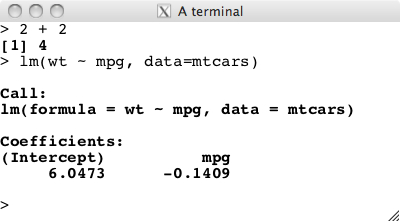
\includegraphics[width=.6\textwidth]{ex-RGtk2-terminal}
  \caption{A basic \R\/ terminal implemented using a \code{gtkTextView} widget.}
  \label{fig:RGtk2-terminal}
\end{figure}


We begin by defining our text view widget and retrieving its
buffer. We also specify a fixed-width font for the buffer.
\begin{Schunk}
\begin{Sinput}
 tv <- gtkTextView()
 tb <- tv$getBuffer()
 font <- pangoFontDescriptionFromString("Monospace")
 tv$modifyFont(font)                     # widget wide
\end{Sinput}
\end{Schunk}

Our main object will be the text buffer which will have only one
view. As there is no built-in method to return a corresponding view
from the buffer, we use the \method{setData}{gtkWidget} method to
associate the view with the buffer.
\begin{Schunk}
\begin{Sinput}
 tb$setData("textview", tv)
\end{Sinput}
\end{Schunk}

We will use a few formatting tags, defined next. We don't need the tag
objects, as we refer to them later by name.
\begin{Schunk}
\begin{Sinput}
 aTag <- tb$createTag(tag.name="cmdInput")
 aTag <- tb$createTag(tag.name="cmdOutput", 
                      weight=PangoWeight["bold"])
 aTag <- tb$createTag(tag.name="cmdError", 
                      weight=PangoStyle["italic"], foreground="red")
 aTag <- tb$createTag(tag.name="uneditable", editable=FALSE)
\end{Sinput}
\end{Schunk}

We define one new mark to mark the prompt for a new line. We
need to be able to identify a new command, and this marks the
beginning of this command.
\begin{Schunk}
\begin{Sinput}
 startCmd <- gtkTextMark("startCmd", left.gravity=TRUE)
 tb$addMark(startCmd, tb$getStartIter()$iter)
\end{Sinput}
\end{Schunk}

We define several functions, which we think of as methods of the text
buffer (not the text view). This first shows how to move the viewport
so that the command line is visibile.
\begin{Schunk}
\begin{Sinput}
 moveViewport <- function(obj) {
   tv <- obj$getData("textview")
   endIter <- obj$getEndIter()
   QT <- tv$scrollToIter(endIter$iter, 0)
 }
\end{Sinput}
\end{Schunk}

There are two types of prompts needed. This function adds a new one or a
continuation one. An argument allows one to specify that the
\code{startCmd} mark is set.
\begin{Schunk}
\begin{Sinput}
 addPrompt <- function(obj, prompt=c("prompt","continue"), 
                       setMark=TRUE) {
   prompt <- match.arg(prompt)
   prompt <- getOption(prompt)
   
   endIter <- obj$getEndIter()
   obj$insert(endIter$iter, prompt)
   tv <- obj$getData("textview")
   if(setMark)
     obj$moveMarkByName("startCmd", endIter$iter)
 }
 addPrompt(tb) ## place an initial prompt
\end{Sinput}
\end{Schunk}

This helper method is used to write the output of a command to the
text buffer. We arrange to truncate large outputs. By passing in the
tag name, we could reuse this function. If we were to streamline the
code for this example, we might use this function to also write out the error
messages, but leave that to the similarly defined function
\code{addErrorMessage} (not shown).


\begin{Schunk}
\begin{Sinput}
 addOutput <- function(obj, output, tagName="cmdOutput") {
   if(length(output) > 100)              # shorten if needed
     out <- c(output[1:100], "...")
 
   endIter <- obj$getEndIter()
   if(length(output) > 0) 
     sapply(output, function(i)  {
       obj$insertWithTagsByName(endIter$iter, i, tagName)
       obj$insert(endIter$iter, "\n", len=-1)
     })
   
   addPrompt(obj, "prompt", setMark=TRUE)
   obj$applyTagByName("uneditable", obj$getStartIter()$iter, 
                      obj$getEndIter()$iter)
   moveViewport(obj)
 }
\end{Sinput}
\end{Schunk}


This next function uses the \code{startCmd} mark and the end of the buffer
to extract the current command. Multi-line commands are handled through
a regular expression which should not be hard-coded to the standard
continue prompt, but for sake of simplicity is.
\begin{Schunk}
\begin{Sinput}
 findCMD <- function(obj) {
   endIter <- obj$getEndIter()
   startIter <- obj$getIterAtMark(startCmd)
   cmd <- obj$getText(startIter$iter, endIter$iter, TRUE)
 
   cmd <- unlist(strsplit(cmd, "\n[+] ")) # hardcoded "+"
   cmd
 }
\end{Sinput}
\end{Schunk}

The following function takes the current command and does the
appropriate thing. It uses a hack (involving \code{grep}) to
distinguish between an incomplete command and a true syntax error. The
\code{addHistory} call refers to a function that is not shown, but is
left to illustrate where one would add to a history stack if desired.

\begin{Schunk}
\begin{Sinput}
 evalCMD <- function(obj, cmd) {
   cmd <- paste(cmd, sep="\n")
   out <- try(parse(text=cmd), silent=TRUE)
   if(inherits(out, "try-error")) {
     if(length(grep("end", out))) {      # unexpected end of input
       ## continue
       addPrompt(obj, "continue", setMark=FALSE)
       moveViewport(obj)
     } else {
       ## error
       addErrorMessage(obj, out)
     }
     return()
   }
   addHistory(obj, cmd)  ## if keeping track of history
   
   out <- capture.output(eval(parse(text = cmd), envir=.GlobalEnv))
   addOutput(obj, out)
 }
\end{Sinput}
\end{Schunk}

The \code{evalCMD} command is called when the \kbd{return} key is
pressed. The \signal{key-release-event} signal passes the event
information through to the second argument. We inspect the key value
and compare to that of the return key. 

\begin{Schunk}
\begin{Sinput}
 ID <- gSignalConnect(tv, "key-release-event", f=function(w, e, data) {
   obj <- w$getBuffer()                  # w is textview
   keyval <- e$getKeyval()
   if(keyval == GDK_Return) {
     cmd <- findCMD(obj)
     if(nchar(cmd) > 0)
       evalCMD(obj, cmd)
   }
   return(FALSE)                         # events need return value
 })
\end{Sinput}
\end{Schunk}
Figure~\ref{fig:RGtk2-terminal} shows the widget placed into a very
simple GUI.



\end{example}


% \begin{example}{Adding parentheses highlighting}{eg:RGtk2:paren-highlight}
%   \SweaveInput{ex-RGtk2-match-parentheses}
% \end{example}

%% insert images or widgets
\paragraph{Inserting non-text items}
If desired, one can insert images and/or widgets into a text buffer,
although this isn't a common use within statistical GUIs. The method
\method{insertPixbuf}{gtkTextBuffer} will insert into a position
specified by an iter a \class{GdkPixbuf} object. In the buffer, this
will take up one character, but will not be returned by
\method{getText}{gtkTextBuffer}. 

Arbitrary child components can also be inserted. To do so an anchor
must first be created in the text buffer. The method
\method{createChildAnchor}{gtkTextBuffer} will return such an anchor, and
then the text view method \method{addChildAtAnchor}{gtkTextView} can
be used to add the child.



\section{Views of tabular and heirarchical data}
\label{sec:RGtk2:tabular-heirarchical-data}

Widgets to create comboboxes, display tabular data values, and to
display tree-like data are treated similarly in \GTK. Each uses the
MVC paradigm and for these, the models are defined similarly.
We begin by discussing the models, then present the various
views. Each view is described by its column, which in turn have their
cells specifed by cell renderers.


\subsection{Tabular  stores and tree stores}
\label{sec:tabular-stores-tree}

\GTK\/ provides list stores and tree stores as models to hold tabular and
heirarchical data to be viewed through various widgets, such as the
combo box or tree view. Like a data frame, each row in these stores
contains data of varying types. The main difference between the two is
that tree stores also have information about about whether a row has
any offspring. The list store is just a tree store where there
are no children of the top-level offspring.

For speed, much greater convenience and familiarity purposes, \pkg{RGtk2} provides a third store
through \constructor{rGtkDataFrame} for storing data frames.

\paragraph{rGtkDataFrame}

\R\/ uses data frames to hold tabular data, where each column is of a
certain class, and each row is related to some observational
unit. This is also the way tree views are organized when no
heirarchical structure is needed. As such it is natural to have a
means to map a data frame into a store for a tree view. The
\constructor{rGtkDataFrame} constructor does this, producing an object
that can be used as the model for a view. This \R-specific
addition to \GTK\/ not only is more convenient, it has the added bonus
of being especially fast. The constructor takes a data frame as an
argument. The column classes are important, so even if this data frame
is empty, it should specify the desired column classes.

The constructor produces an object of class \class{RGtkDataFrame}
which has a few methods defined for it. The familiar S3 methods
\method{[}{RGtkDataFrame}, \method{[\ASSIGN}{RGtkDataFrame},
\method{dim}{RGtkDataFrame}, and \method{as.data.frame}{RGtkDataFrame}
are defined. The \code{dimnames} attributes are kept, but have no
well-defined meaning
for this model. The \code{[$<$-} method does not have quite the same
functionality, as it does for a data frame. Columns can not be removed
by assigning values to \code{NULL}, column types
should not be changed which can be an issue with coercion to character from numeric
say, rows can not be dropped. To add a new column or row, the methods
\method{appendColumns}{rGtkDataFrame} and
\method{appendRows}{rGtkDataFrame} may be used, where the new column
or row may be given as the argument.

To remove rows from this model, the \method{setFrame}{rGktDataFrame}
method can be used to specify the new data. This method can also be used
to replace the existing data in the model with a new data
frame. There are few issues though. If the new data frame has more
rows or columns, then the appropriate \code{append} method should be
used first. As well, one should not change the column classes with the
new frame, as views of the model may be expecting a certain class of data.

\begin{example}{Defining and manipulating a data store}{eg-RGtk2-manipulate-rGtkDataframe}
  The basic data frame methods are similar.
\begin{Schunk}
\begin{Sinput}
 data(Cars93, package="MASS")            # mix of classes
 model <- rGtkDataFrame(Cars93)
 model[1, 4] <- 12
 model[1, 4]                              # get value
\end{Sinput}
\begin{Soutput}
[1] 12
\end{Soutput}
\end{Schunk}
Factors are treated differently from character values, as is done with
data frames, so assignment to a factor must be from one of the
possible levels.

To change the backend data, we can use the \code{SetFrame} method:
\begin{Schunk}
\begin{Sinput}
 QT <- model$setFrame(Cars93[1:5, 1:5])
\end{Sinput}
\end{Schunk}
\end{example}


\paragraph{List stores and tree stores}
Although the \code{rGtkDataFrame} model is very useful, there are
times when it can't be employed. List stores can be used when the
underlying data contains values that can not be stored in a data frame
(such a images) and tree stores are used for heirarchical data. 

%% construction
A tree store or list store is constructed using
\constructor{gtkTreeStore} or  \constructor{gtkListStore}. Both are
interfaces for the abstract \class{GtkTreeModel} class. The
column types are specified through a character vector at the time of
construction. The specification uses ``GTypes'' such as
\code{gchararray} for character data, \code{gboolean} for logical data,
\code{gint} for integer data, \code{gdouble} for numeric data, and
\code{GObject} for \GTK\/ objects, such as pixbufs.

%% iters vs. paths
\paragraph{Iterators and tree paths}
Similar to a text buffer, a list store uses transient iterators to
refer to position -- in this case the row -- within a store. One can
also refer to position through a path, which for a list store is
essentially the row number, $0$-based, as a character; and for a tree
is a colon-separated set of values referring to the offspring
(\qcode{a:b:c} indicates the \code{c}th child of the \code{b}th child
of \code{a}).  A third way, through a row reference, is not discussed
here.

%% paths
A \class{GtkTreePath} object is created by the constructor
\code{gtkTreePathNewFromString} which takes a string specifying the
position. To retrieve this string from a path object, the
\method{toString}{gtkTreePath} method can be used.

%% iters
Paths are convenient, as they are human readable, but iterators are
empolyed by the various methods and more easily allow the programmer
to traverse the store. One can flip between the two
representations. The iterator referring to the path can be returned by
the method \method{getIterFromString}{gtkTreeModel}. The method
\method{getStringFromIter}{gtkTreeModel} will return the string. The
tree path object itself is returned by the method
\method{getPath}{gtkTreeModel}.  In \pkg{RGtk2} iterators are lists
with component \code{retval} indicating if this is a valid iterator
and a component \code{iter} holding the object of the
\class{GtkTreeIter} class.

%% adding to a storex
\paragraph{Adding values to a store}
Values are added to and returned from a store by specifying the row
and column for the value. The row is specified by an iterator and the
columns by its index, $0$-based.  The method
\method{setValue}{gtkListStore} is used to specify value by value,
whereas an entire row can be assigned through the
\method{set}{gtkTreeStore} method. The former has arguments
\code{iter}, \code{column}, \code{value}, in that order; the latter
has no \code{column} or \code{value} argument. Instead, \code{Set}
uses positional arguments to specify the column and the value. The
column index appears as an even argument (say $2k$) and the
corresponding value in the odd argument (say $2k+1$).  When calling
\code{setValue} or \code{set} the iterator updates to the next row
Values are returned by the \method{getValue}{gtkListStore} method,
a list with component \code{value} storing the value.

\paragraph{Finding iterators}
For a list or tree model, an iterator for the first child is returned
by \method{getIterFirst}{gtkTreeStore}. This iterator corresponds to
the path \qcode{0}.
The \method{append}{gtkStore}
method for the store returns an iterator indicating the next value at
the end of the store (this is slightly different from the \GTK\/ function which
modifies an iterator passed as an argument).  The
\method{prepend}{gtkTreeStore} method is similar, only returning an
iterator pointing to the initial row.  Other methods allow for
specifying postion relative to some row. The
\method{insert}{gtkListStore} method is used to return an iterator
that allows one to insert a row at a position specified to its
\code{position} argument. (The \code{Prepend} method is similar to
using \code{postion=0}). To avoid the two-step approach of getting the
iterator, then assigning the value, the method
\method{insertWithValues}{gtkListStore} can be used, where values are
specified as with the \code{Set} method.  The
\method{insertBefore}{gtkListStore}, and
\method{insertAfter}{gtkListStore}, methods take an iterator,
\code{sibling} and will return an iterator indicating the postion just
before or after the sibling.




\begin{example}{Appending to a list store}{eg:RGtk2:list-store}
  To illustrate, to create a simple list store to hold a column
of text we have:  
\begin{Schunk}
\begin{Sinput}
 lstore <- gtkListStore("gchararray")
 for(i in 1:nrow(Cars93)) {
   iter <- lstore$append()
   if(is.null(iter$retval)) 
     lstore$setValue(iter$iter, 0, Cars93[i,1])
 }
\end{Sinput}
\end{Schunk}
To retrieve a value, we have this example to get the first one in the store:
\begin{Schunk}
\begin{Sinput}
 iter <- lstore$getIterFirst()           # first row
 lstore$getValue(iter$iter, column = 0)
\end{Sinput}
\begin{Soutput}
$retval
NULL

$value
[1] "Acura"
\end{Soutput}
\end{Schunk}
\end{example}

\paragraph{Adding heirarchical information}

For a tree store, the methods \method{append}{gtkTreeStore},
\method{prepend}{gtkTreeStore} etc. are similar to that for a list
store with the difference being that a
\argument{parent}{gtkTreeStoreAppend} argument is used for tree stores
to specify in iterator for the parent of the new row, thereby creating
the heirarchical structure of a tree.


\begin{example}{Defining a tree}{eg:RGtk2:tree-store}
  As an application, we can create a tree with parents the car
  manufacturers in the \code{Cars93} data set, and children the makes
  of their cars, as follows:
\begin{Schunk}
\begin{Sinput}
 tstore <- gtkTreeStore("gchararray")
 Manufacturers <- Cars93$Manufacturer
 Makes <- split(Cars93[,"Model"], Manufacturers)
 for(i in unique(Manufacturers)) {
   piter <- tstore$append()              # parent
   tstore$setValue(piter$iter, column=0, value=i)
   for(j in Makes[[i]]) { 
     sibiter <- tstore$append(parent=piter$iter) # child
     if(is.null(sibiter$retval)) 
       tstore$setValue(sibiter$iter,column=0, value=j)
   }
 }
\end{Sinput}
\end{Schunk}
To retrieve a value from the tree store using its path we have:
\begin{Schunk}
\begin{Sinput}
 iter <- tstore$getIterFromString("0:0") #  the 1st child of root
 tstore$getValue(iter$iter,column=0)$value
\end{Sinput}
\begin{Soutput}
[1] "Integra"
\end{Soutput}
\end{Schunk}
\end{example}


%% Manipulating rows
\paragraph{Manipulating rows}
Rows within a store can be rearranged using the methods
\method{swap}{gtkTreeStore} to swap rows referenced by their
iterators; \method{moveAfter}{gtkTreeStore} to move one row after
another, both referenced by iterators, although if the last is blank,
the end of the store is assumed; and
\method{moveBefore}{gtkTreeStore}, where if the second iterator is
blank the first position is assumed. To totally reorder the store, the
\method{reorder}{gtkTreeStore} method is available. Its
\argument{new.order}{gtkTreeStore} argument specifies the new
order as row indices. For tree stores, these rows are the children of the
\argument{parent}{gtkTreeStoreReorder} argument.

%% clearing contents
Once added, rows may be removed using the
\method{remove}{gtkTreeStore} method. The iterator for the row to
delete is given as an argument. The store's entire contents can be
removed by its \method{clear}{gtkTreeStore} method.


%% Traversing
\paragraph{Traversing the store}
An iterator points to a row in a tree or list store. For both lists
and trees, an interator pointing to the next row (at the same level
for trees) is produced by the method
\method{iterNext}{gtkTreeStore}. This method returns \code{FALSE} if
no next row exists. Otherwise, it updates the iterator in place. (That
is, calling \command{store\$iterNext(iter\$iter)} updates \code{iter},
despite it not being assigned to.) The path method \method{prev}{gtkTreePath}
will point to the previous child at the same depth in a tree, but no
such method is defined for iterators. One could be, for example the
following will do so for both list and tree stores.

\begin{Schunk}
\begin{Sinput}
 gtkTreeModelIterPrev <- function(object, iter) {
   path <- object$getPath(iter)
   ret <- path$prev()
   if(ret)
     return(list(retval=NULL, iter=object$getIter(path)$iter))
   else
     return(list(retval=FALSE,iter=NA))
 }
\end{Sinput}
\end{Schunk}

For trees, the method \method{iterParent}{gtkTreeModel} returns an
iterator to point to the parent row, if no parent is found. The
\code{retval} component is \code{FALSE}.
There are several methods when a row has children.  The
method \method{iterHasChild}{gtkTreeModel} returns a logical
indicating if a row has children. The method
\method{iterChildren}{gtkTreeModel} returns an iterator to point to
the first child of parent. If no child exists, the \code{retval}
component is \code{FALSE}. If an iterator for the $n$th child is desired, the
method \method{iterNthChild}{gtkTreeModel} can be used. Again, it returns
an iterator referring to the $n$th child, or has a \code{retval} of
\code{FALSE} if
none exists. To find the number of children, the method
\method{iterNChildren}{gtkTreeModel} is provided. This method returns
$0$ if there are no children.

\begin{figure}
%%  \centering
  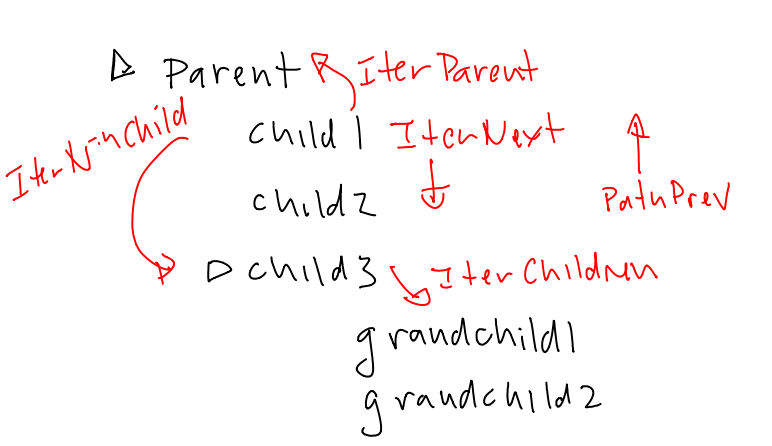
\includegraphics[width=.7\textwidth]{traverse-tree}
  \caption{[REPLACEME!] Graphical illustration of the functions used by iters to traverse a tree store. }
  \label{fig:traverse-iter}
\end{figure}

\subsection{Cell renderers}
\label{sec:RGtk2:cellrenderers}
The various views ultimately display the information in the model
column by column (a combobox having one column). Within each column,
the display is controlled by cell renderers, which are used to specify
how each cell is layed out. Cell renderers are used whenever the 
\code{gtkCellLayout} interface is implemented, such as with comboboxes
and tree views, but also other widgets not discussed here.

A cell renderer is customized by adjusting its attributes. These
attributes are documented in the help pages for the corresponding
constructor. These attributes can be set to one value for all rows, or
can be set to depend on a corresponding row in the model. The latter
allows them to change from cell to cell. For example, the \code{text}
attribute of the text cell renderer would usually get its values from
the model, as that would vary from cell to cell, but a background
color (\code{background}) might be common to the column. The
\method{addAttribute}{gtkCellLayout} method is used to associate a
column in the store with a cell renderer's attribute.

There are many different cell renderers, we mention first the text and
pixbuf renderer, as they are commonly used in comboboxes. With the
discussion of tree views, we mention others.

%% text/ numbers
\paragraph{Text cell renderers}
The \constructor{gtkCellRendererText} constructor is used to display
text and numeric values. Numeric values are shown as strings, but are
not converted in the model.  For the text renderer, important
properties are \code{text} to indicate the column in the data store
that the text for the cell is to come from, \code{font} to specify the
font from a string, \code{size} for the font size, \code{background}
for the background color and \code{foreground} for the text color (as
strings).

To display right-aligned text in a Helvetica font, the following could be used:
\begin{Schunk}
\begin{Sinput}
 cr <- gtkCellRendererText()
 cr['xalign'] <- 1                       # default 0.5 = centered
 cr['family'] <- "Helvetica"  
\end{Sinput}
\end{Schunk}
The \code{wrap} attribute can be specified as \code{TRUE}, if the
entries are expected to be long. There are several other attributes that can
changed. 

%% pixbuf
\paragraph{Pixbuf cell renderers}
Graphics can be added to the cell with the renderer
\constructor{gtkCellRendererPixbuf}. The graphic can be spepcified by
its \code{stock-id} attribute as a character string, or
\code{icon-name} for a themed icon. It can also be specifed as an
image object, through the \code{pixbuf} attribute. Pixbuf objects can
be placed in a list store using the \code{GObject} type. A simple use,
might be the following:
\begin{Schunk}
\begin{Sinput}
 cr <- gtkCellRendererPixbuf()
 cr['stock.id'] <- "gtk-ok" ## or from a column in a model
\end{Sinput}
\end{Schunk}


% <<CellRendererExample>>=
% cr <- gtkCellRendererText()
% cr['family'] <- "Helvetica"             # font family for whole column
% cr['background'] <- "goldenrod"         # background color for column
% crp <- gtkCellRendererPixbuf();         # a pixbuf
% crp['xalign'] <- 0
% @

% Cellrenderers define how data is to be displayed. The binding of the
% data to the cell renderer is handled by the view, not the
% cellrenderer.

\subsection{Combo boxes}
\label{sec:RGtk2:combobox}

The basic combo box usage was discussed in
Section~\ref{sec:RGtk2:basic-combobox}, here we discuss more
complicated comboboxes that use a model for the backend This data is
tabular and may be kept in a \function{rGtkDataFrame} instance or a
list store.  

The basic \constructor{gtkComboBoxEntryNewWithModel} constructor
allows one to specify the model, and a column where the values are
found. For this, the cell renderers (below) are not needed.

If some layout of the values in the combobox is desired, such as adding an image,
then the constructor
\constructor{gtkComboBox} is used. The model may be specified at the time of
construction through the optional \argument{model}{gtkComboBox}
argument.  This model may be changed or set through the
\method{setModel}{gtkComboBox} method and is returned by
\method{getModel}{gtkComboBox}.

The constructor \constructor{gtkComboBoxEntry} returns a combobox
widget that allows the user to add their own values. This constructor
does not allow the model to be specified, so the \code{SetModel}
method must be used. The editable combobox uses a \code{gtkEntry}
object, which can be accessed directly through the
\method{getChild}{gtkBin} method of the combobox.

\paragraph{Cellrenderers}
Comboboxes display rows of data, each row referred to as a cell. In \GTK\/ each cell is like a box
container and can show different bits of information, like an image or
text. Each bit of information is presented by a cellrenderer.
Cellrenderers are added to the combo box by its
\method{packStart}{gtkCellLayout} method. As with box containers, more
than one cell renderer can be added per row.

To specify the data from the model to be
displayed, the \method{addAttribute}{gtkCellLayout} method maps
columns of the model to attributes of the cellrenderer. 



%% get value from widget
\paragraph{Retrieving the selected value}
For a non-editable combobox, the selected value may be retrieved by
index or by iterator. The \method{getActive}{gtkComboBox} method
returns the index of the current selection, $0$-based. The value is $-1$
if no selection has been made. The
\method{getActiveIter}{gtkComboBox} method returns an iterator
pointing to the row in the data store. If no row has been selected,
the \code{retval} component of the iterator is \code{FALSE}. These may
be used with the data store to retrieve the value. The data store
itself is returned by the \method{getModel}{gtkComboBox} method.

To set the combobox to a certain index is done through the
\method{setActive}{gtkComboBox} method, using a $0$-based index to
specify the row.

For editable comboboxes, one can first get the entry widget then call
its \code{GetText} method. The \code{SetText} method of the entry
widget would be used to specify the text.


%% signals
\paragraph{Signals}
When a user selects a value with the mouse, the \code{changed} signal
is emitted. For editable combo boxes, the user may also make changes
by typing in the new value. The underlying widget is a \code{gtkEntry}
widget, so the signal \code{changed} is emitted each time the text is
changed and the signal \code{activate} is emitted by the
\code{gtkEntry} widget when the \kbd{enter} key is pressed. One binds to
the signal of the entry widget, not the combobox widget, to have a
callback for that event.


\begin{example}{Modifying the values in a combobox}{eg-RGtk2-combobox-dynamic}
This example shows how to use two comboboxes to achieve a useful
task. That being, allowing the user a means to select from the
available variables in a data frame. We use a \code{rGtkDataFrame}
model for each, but for one use the basic constructor and the other
the more involved, as an illustration.
\begin{Schunk}
\begin{Sinput}
 data("Cars93", package="MASS")
 dfNames <- c("mtcars", "Cars93")
 dfModel <- rGtkDataFrame(dfNames)
 dfCb <- gtkComboBoxEntryNewWithModel(dfModel, text.column=0)
\end{Sinput}
\end{Schunk}

The variable names are initially just an empty string. We use an
\code{rGtkDataFrame}  as the
model and also specify a cell renderer to view the data.

\begin{Schunk}
\begin{Sinput}
 variableNames <- character(0)
 varModel <- rGtkDataFrame(variableNames)
 varCb <- gtkComboBoxNewWithModel(varModel)
 cr <- gtkCellRendererText()
 varCb$packStart(cr)
 varCb$addAttribute(cr, "text", 0)
\end{Sinput}
\end{Schunk}

Our basic GUI uses a table for layout. Comboboxes fill and expand to fill the cell.
\begin{Schunk}
\begin{Sinput}
 tbl <- gtkTableNew(rows=2, columns=2, homogeneous=FALSE)
 tbl$attach(gtkLabel("Data frame"), left.attach=0,1, top.attach=0,1)
 tbl$attach(dfCb, left.attach=1,2, top.attach=0,1)
 tbl$attach(gtkLabel("Variables"), left.attach=0,1, top.attach=1,2)
 tbl$attach(varCb, left.attach=1,2, top.attach=1,2)
\end{Sinput}
\end{Schunk}
This callback will be used for both the entry widget and the combobox,
so we first check which it is and if it is the combobox, we get the
entry widget from it. To update the display we replace the model. The
option of replacing the frame within the current model requires us to
be careful when adding additional rows.

\begin{Schunk}
\begin{Sinput}
 newDfSelected <- function(varCb, w, ...) {
   if(inherits(w, "GtkComboBox"))        # get entry widget
     w <- w$getChild()
   val <- w$getText()
   df <- try(get(val, envir=.GlobalEnv), silent=TRUE)
   if(!inherits(df, "try-error") && is.data.frame(df)) {
     nms <- names(df)
     ## update model
     newModel <- rGtkDataFrame(nms)
     varCb$setModel(newModel)
     varCb$setActive(-1)
   }
 }
\end{Sinput}
\end{Schunk}
Our callbacks for the data frame combobox simply call the above
function. As for the variable combobox, we show how to get the
selected value, but for no real purpose.
\begin{Schunk}
\begin{Sinput}
 QT <- gSignalConnect(dfCb, "changed", f=newDfSelected,
                      user.data.first=TRUE,
                      data=varCb)
 QT <- gSignalConnect(dfCb$getChild(), "activate", f=newDfSelected,
                      user.data.first=TRUE,
                      data=varCb)
 QT <- gSignalConnect(varCb, "changed", f=function(w, ...) {
   model <- w$getModel()
   iter <- w$getActiveIter()
   val <- model$getValue(iter$iter, column=0)
   print(val$value)                      # add real purpose
 })
\end{Sinput}
\end{Schunk}
\end{example}

\begin{example}{A color selection widget}{eg:RGtk2:combobox}
%%
This examples shows how a combobox can be used as an alternative to
\function{gtkColorButton} to select a color. We use two cellrenderers
for each row, one to hold an image and the other a text label.


This function uses the \pkg{grid} package to produce a graphic that
will read into the pixbuf.

\begin{Schunk}
\begin{Sinput}
 require(Cairo)
 makePixbufFromColor <- function(color) {
   filename <- tempfile()
   Cairo(file=filename, width=25,height=10)
   grid.newpage()
   grid.draw(rectGrob(gp = gpar(fill = color)))
   dev.off()
   image <- gdkPixbufNewFromFile(filename)
   unlink(filename)
   return(image$retval)
 }
\end{Sinput}
\end{Schunk}

Our data store has one column for the pixbuf and one for the color
text. The pixbuf is stored using the \code{GObject} class.

\begin{Schunk}
\begin{Sinput}
 store <- gtkListStore(c("GObject","gchararray"))
\end{Sinput}
\end{Schunk}

This loop adds the colors and their name to the data store.
\begin{Schunk}
\begin{Sinput}
 theColors <- palette()                  # some colors
 for(i in theColors) {
   iter <- store$append()
   store$setValue(iter$iter, 0, makePixbufFromColor(i))
   store$setValue(iter$iter, 1, i)
 }
\end{Sinput}
\end{Schunk}

Next we define the combobox using the store as the model. There are
two cell renderers to add.
\begin{Schunk}
\begin{Sinput}
 combobox <- gtkComboBox(model=store)
 ## pixbuf
 crp <- gtkCellRendererPixbuf(); crp['xalign'] <- 0
 combobox$packStart(crp, expand=FALSE)                
 combobox$addAttribute(crp, "pixbuf", 0)
 ## text
 crt <- gtkCellRendererText(); 
 crt['xpad'] <- 5                        # give some space
 combobox$packStart(crt)
 combobox$addAttribute(crt, "text", 1)
\end{Sinput}
\end{Schunk}


% This shows how the method \method{GetActiveIter}{gtkComboBox}
% indicates the selected value, which can be used by the
% \method{GetValue}{gtkTreeStore} method of the  data store to retrieve
% the value.
% <<changedsignal>>=
% ID <- gSignalConnect(combobox, "changed",
%               f = function(cb, data) {
%                 store <- cb$getModel()
%                 iter <- cb$getActiveIter()
%                 if(iter$retval) {
%                   val <- store$getValue(iter$iter,1)$value 
%                   print(val)
%                 }
%                 return(TRUE)
                
%               })
% @ 
% \end{example}



% \begin{example}{Editable combo box}{eg:RGtk2:editable combo box}

%   This example is similar to the previous one, except it adds the
%   ability to edit the value in the combobox.

%   The \argument{text.column}{gtkComboBoxEntryNewWithModel} argument in
%   the constructor specifies which column in the data store contains
%   the text. We do not need a cell renderer to display the text.

% <<>>=
% comboentry <- gtkComboBoxEntryNewWithModel(store, text.column = 1)
% @ 

% To draw the image next to the text is similar to before.

% <<>>=
% crp <- gtkCellRendererPixbuf(); crp['xalign'] <- 0
% comboentry$packStart(crp, expand=FALSE)                 # icon first
% comboentry$addAttribute(crp, "pixbuf", 0)
% @ 

% We need to call the \method{Show}{gtkWidget} method for this widget to
% be visible.
% <<>>=
% comboentry$show()
% @ 

% Again, we simply add the widget to a top-level window.
% <<>>=
% win <- gtkWindow();win$setTitle("Combo box with entry")
% win$add(comboentry)
% @ 


% These two callbacks show how to attach a callback to changes due to
% either selecting a value from the available values or pressing
% \kbd{enter} after entering a value.

% <<>>=

% ID <- gSignalConnect(comboentry, "changed", # changed via popup
%                f = function(cb, data) {
%                  if(cb$getActive() != -1)
%                    print(cb$getChild()$getText())
%                  return(TRUE)
%                })
% ## just enter will call handler. Widget is gtkEntry instance
% ID <- gSignalConnect(comboentry$getChild(), "activate", # on entry
%               f = function(w, data) {
%                   print(w$getText())
%                 return(TRUE)
%               })

% @ 
\end{example}


\subsection{Text entry widgets with completion}
\label{sec:RGtk2:entry-completion}

A common alternative to a combobox, implemented on many websites, is to add the completion features to a
\constructor{gtkEntry} instance. When a user types a partial match,
all available matches are offered to select from. To implement completion, one creates
a completion object with the constructor
\constructor{gtkEntryCompletion}. The values to complete from are
stored in a model, the example uses an \code{rGtkDataFrame} instance,
which is assigned to the completion object through its
\method{setModel}{gtkEntryCompletion} method. To set the completion
for the entry widget, the entry widget's
\method{setCompletion}{gtkEntry} method is used. The
\code{text-column} property is used to specify which column in
the model is used to find the matches, we use the method
\code{SetTextColumn} in the example to set this.


There are several properties that can be adjusted to tailor the
completion feature, we metion some of them. Setting the property
\code{inline-selection} to \code{TRUE} will place the completion
suggestion to the entry inline as the completions are scrolled
through; \code{inline-completion} will add the common prefix
automatically to the entry widget; \code{popup-single-match} is a
logical indicating if a popup is displayed on a single match;
\code{minimum-key-length} takes an integer specifying the number of
characters needed in the entry before completion is checked, the
default is $1$.

By default, the rows in the data model that match the
current value of the entry widget in a case insensitive manner are displayed. This
matching function can be overridden by setting a new function through
the \method{setMatchFunc}{gtkEntryCompletion} method. The signature of
this function is the completion object, the string from the entry
widget (lower case), an interator pointing to a row in the model and optionally
user data that is passed through the \code{func.data} argument of the
\code{SetMatchFunc} method. This method should return \code{TRUE} or
\code{FALSE} depending on whether that row should be displayed in the
set of completions.


\begin{example}{Text entry with completion}{eg:RGtk2:text-entry-comletion}
This example illustrates the basic steps to add completion to a text entry.


The two basic widgets are defined as follows:
\begin{Schunk}
\begin{Sinput}
 entry <- gtkEntry()
 completion <- gtkEntryCompletionNew()
 entry$setCompletion(completion)
\end{Sinput}
\end{Schunk}

We will use a \code{rGtkDataFrame} instance for our completion model,
taking a convenient list of names for our example.
We set the completion objects's model and text column using the
similarly named methods, and then set some properties to customize how
the completion is handled.
\begin{Schunk}
\begin{Sinput}
 store <- rGtkDataFrame(data.frame(name=I(state.name)))
 completion$setModel(store)
 completion$setTextColumn(0)             # which column in model
 completion['inline-completion'] <- TRUE # inline with text edit
 completion['popup-single-match'] <- FALSE
\end{Sinput}
\end{Schunk}

If we wanted to set a different matching function, one would do
something along the lines of the following where \function{grepl} is
used to indicate any match, not just the initial part of the
string. We get the string from the entry widget, not the value passed
in, as that has been standardized to lower case.

\begin{Schunk}
\begin{Sinput}
 f <- function(comp, str, iter, user.data) {
   model <- comp$getModel()
   rowVal <- model$getValue(iter, 0)$value   # column 0 in model
   
   str <- comp$getEntry()$getText()      # case sensitive
   grepl(str, rowVal)
 }
 QT <- completion$setMatchFunc(func=f)
\end{Sinput}
\end{Schunk}

\begin{Schunk}
\begin{Sinput}
 ## Our basic GUI is basic:
 w <- gtkWindow(show=FALSE)
 w$setTitle("Test of entry with completion")
 w$add(entry)
 w$showAll()
\end{Sinput}
\end{Schunk}



\end{example}



\subsection{Tree Views}
\label{sec:RGtk2-tree-view}

%% intro
Both tabular data and tree-like data are displayed through tree
views. The visual difference is that a trigger icon appears in rows which
represent parents with children. When these are expanded, the
children are indicated by indentation. The children are all displayed
in a consistent tabular format.

%% constructor
A tree view is constructed by \constructor{gtkTreeView}. The
\argument{model}{gtkTreeView} can be used to specify the underlying
model. If not specified at the time of construction, the
\method{setModel}{gtkTreeView} can be used. The accompanying
\method{getModel}{gtkTreeView} model returns the model from the view.

%% tree view properties
Tree views have several properties. The \code{headers-clickable}
property, when set to \code{TRUE}, allows the column headers to
receive mouse clicks. This is used for sorting, when the underlying
data store allows for that. The tree view widget can popup a search
box when the user types \kbd{control-f} if the property
\code{enable-search} is \code{TRUE} (the default). To turn on
searching, a column needs to be specified through the
\code{search-column} property. Rows may be rearranged through
drag-and-drop if the \code{reorderable} property is set to
\code{TRUE}. The \code{rules-hint}, if \code{TRUE}, will instruct the
theme that the rows hold associated data. Themes will typically use this
information to stripe alternating rows.


%% treeviewcolumns
\paragraph{Tree view columns}
For speed purposes, the rendering of a tree view centers around the
display of its columns. Each column is displayed through a tree view
column, given by the \constructor{gtkTreeViewColumn}.

%% basic properties
One can set basic properties of the column. Each column has an
optional header that can contain a title or even an arbitrary
widget. The \method{setTitle}{gtkTreeViewColumn} method is used to set
the title. This area can be \qcode{clickable}, in which case this area
receives mouse clicks. This is most commonly used to allow sorting of
the column by clicking on the headers, but can also be used to add
popup menus (with a bit of wizardry).

The property \qcode{resizable} determines wheter the user can resize
the column, by dragging with the mouse. The size properties
\qcode{width}, \qcode{min-width}, and \qcode{fixed-width} control the
size.

The visibility of the column can be adjusted through the
\method{setVisible}{gtkTreeViewColumn} method. 


Tree view columns are added to the tree view with the
method \method{insertColumn}{gtkTreeView}. The
\argument{column}{gtkTreeViewInsertColumn} argument specifies the tree
view column, and the \argument{position}{gtkTreeViewInsertColumn}
argument the column to insert into ($0$-based). A column can be moved
with the \method{moveColumnAfter}{gtkTreeView} method, and removed
with the \method{removeColumn}{gtkTreeView} method. The tree view's
\method{getChildren}{gtkTreeView} method returns a list containing all
of the tree view columns.

%% cell renderers
\paragraph{More on cell renderers}

In addition to the text and pixbuf cell renderers discussed in
Section~\ref{sec:RGtk2:combobox}, there are cell renderers that allow
one to display other types of data available for the tree view widget.
Some only make sense if the underlying data is to be edited, for
example the combobox renderer, for these, the \code{editable}
attribute for the cell renderer
should be set to \code{TRUE}.


As with comboboxes, the mapping of values in the data store to the
attributes of a cell render is done by the
\method{addAttribute}{gtkCellLayout} method of the tree view column.


\paragraph{Toggle cell renderers}
Binary data can be represented by a toggle. The
\constructor{gtkCellRendererToggle} will create a check box in the
cell, that  will look checked or not depending on the value of its
\code{active} attribute. If this value is found in a boolean column of
the model, then changes to the model will be reflected in the state of
the GUI. However, the programmer must propogate changes to the GUI (the
view) back to the model. The \signal{toggled} signal is emitted when
the state is changed. The \code{activatable} attribute for the cell
must be \code{TRUE} in order for it to receive user input.

\begin{Schunk}
\begin{Sinput}
 cr <- gtkCellRendererToggle()
 cr['activatable'] <- TRUE               # cell can be edited
 cr['active'] <- TRUE
 QT <- gSignalConnect(cr, "toggled", function(w, path) {
   print(as.numeric(path) + 1) ## the row
 })
\end{Sinput}
\end{Schunk}

%% combo
\paragraph{Combobox cell renderers}
A cell can show a combobox for selection. The
\constructor{gtkCellRendererCombo} produces the object. Its
\code{model} attribute is set to give the values to choose from. The
attribute \code{has-entry} can be set to \code{TRUE} to allow a user
to enter values, if \code{FALSE} they can only select from the
available ones. 

\begin{Schunk}
\begin{Sinput}
 cr <- gtkCellRendererCombo()
 store <- rGtkDataFrame(state.name)
 cr['model'] <- store
 cr['text-column'] <- 0
 cr['editable'] <- TRUE                  # needed
\end{Sinput}
\end{Schunk}

%% progress bars
\paragraph{Progress bar cell renderers}
A progress bar can be used to display the percentage of some task. The
\constructor{gtkCellRendererProgress} function returns the cell
renderer. Its \code{value} attribute takes a value between $0$ and
$100$ indicating the amount finished, with a default value of
$0$. Values out of this range will be signaled by an error message.  The
\code{orientation} property, with values from
\code{GtkProgressBarOrientation}, can adjust the direction that the
bar grows.  For example,

\begin{Schunk}
\begin{Sinput}
 cr <- gtkCellRendererProgress()
 cr["value"] <- 50                       # fixed 50%
 cr['orientation'] <- "right-to-left"
\end{Sinput}
\end{Schunk}

%% numbers
\paragraph{Cell data functions}
Formatting numbers is a bit trickier, as the cell renderer properties
are geared around text values. For example, to align floating point
numbers one can do so in the model and then display as text. However,
to do so through the cell rendererer requires one to get the value
from the model and modify it before the cell rendererer gets it. For
this, a cell data function is used, and not with comboboxes, but only
tree views. A cell data function has arguments pointing to a tree view
column, the cell renderer, the model, an
iterator pointing to the row in the model and a data argument for user
data. The function should set the appropriate attributes of the cell
renderer. For example, this function could be used to format floating
point numbers:
\begin{Schunk}
\begin{Sinput}
 func <- function(viewCol, cellRend, model, iter, data) {
   curVal <- model$GetValue(iter, 0)$value
   fVal <- sprintf("%.3f", curVal)
   cellRend['text'] <- fVal
   cellRend['xalign'] <- 1
 }
\end{Sinput}
\end{Schunk}

%% This function will be set for the tree view column and illustrated in Example~\ref{ex:RGtk2:rGtk2DataFrame}.



%% editable cells \paragraph{Editable cells} When the \code{editable}
property of a text cell (or \code{activatable} property of a toggle
cell) is set to \code{TRUE}, then the cell contents can be
changed. This allows the user to make changes to the underlying model
through the GUI. Although the view automatically reflects changes made
to the model, the reverse is not true. A callback must be assigned to
the \code{editable} (\code{toggled}) signal for the cell renderer to
imlement the change. The callback for the \qcode{editable} signal has
arguments \code{renderer}, \code{path} for the path of the selected
row (as a string), and \code{new.text} containing the value of the edited text as a
string. The tree view and which column was edited are not passed in by
default. These can be passed through the user data arugment, or set as
data for the widget if needed within the callback.
\begin{Schunk}
\begin{Sinput}
 cr['editable'] <- TRUE
 ID <- gSignalConnect(cr, "edited", 
                      f=function(cr, path, newtext, data) {
                        curRow <- as.numeric(path) + 1
                        model <- data$model
                        curCol <- data$column
                        model[curRow, curCol] <- newtext
                      }, data=list(model=store, column=1))
\end{Sinput}
\end{Schunk}

Users may expect that once a cell is edited, the next cell is then set
up to be edited. In order to do this, one must set the cursor to the
appropriate place and set the state to editing. This is done through
the tree view's \method{setCursor}{gtkTreeView} method. The
\code{path} argument takes a tree path instance, the \code{column}
argument is for a tree view column object, and the flag
\code{start.editing} should be set to \code{TRUE} to initiate
editing. The tree view method \method{getColumn}{gtkTreeView} can be
used to get the tree view column by index ($0$-based) and the path
object can be found from a string through \function{gtkTreePathNewFromString}.


% \begin{example}{A basic usage of displaying a data frame using a tree view}{ex:RGtk2-minimal-rGtkDataFrame}
%   \SweaveInput{ex-RGtk2-minimal-rGtkDataFrame}
% \end{example}

\begin{example}{Displaying text columns in a tree view}{ex:RGtk2-add-toggle-to-df}
This example shows how to select one or more rows from a data frame
that contains some information. We write it so any data frame could be
used, although in the specific case we show a list of the installed
packages that can be upgraded from CRAN.


To get the installed packages that can be upgraded, we use some of the
functions provided by the  \pkg{utils} package.
\begin{Schunk}
\begin{Sinput}
 avail <- available.packages()
 installed <- installed.packages()
 tmp <- merge(avail, installed, by="Package")
 need.upgrade <- with(tmp, as.character(Version.x) != as.character(Version.y))
 d <- tmp[need.upgrade, c(1, 2, 16, 6)]
 names(d) <- c("Package", "Available", "Installed", "Depends")
\end{Sinput}
\end{Schunk}


This function will be called on the selected rows. The \code{print}
call would be replaced with something more reasonable, such as a call
to \function{install.packages}.
\begin{Schunk}
\begin{Sinput}
 doThis <- function(d) print(d)
\end{Sinput}
\end{Schunk}

The rest of this code is independent of the details of \code{d}. We first
append a column to the data frame to store the selection information.
\begin{Schunk}
\begin{Sinput}
 n <- ncol(d)
 nms <- names(d)
 d$.toggle <- rep(FALSE, nrow(d))
 store <- rGtkDataFrame(d)
\end{Sinput}
\end{Schunk}

Our tree view shows each column using a simple text cell renderer,
except for an initial one where the user can select the packages they
want to call \code{doThis} on.
\begin{Schunk}
\begin{Sinput}
 view <- gtkTreeView()
 # add toggle
 togglevc <- gtkTreeViewColumn()
 view$insertColumn(togglevc, 0)
\end{Sinput}
\begin{Soutput}
[1] 1
\end{Soutput}
\begin{Sinput}
 cr <- gtkCellRendererToggle()
 togglevc$packStart(cr)
 cr['activatable'] <- TRUE
 togglevc$addAttribute(cr, "active", n)
 gSignalConnect(cr, "toggled", function(cr, path, user.data) {
   view <- user.data
   row <- as.numeric(path) + 1
   model <- view$getModel()
   n <- dim(model)[2]
   model[row, n] <- !model[row, n]
 },
                data=view)
\end{Sinput}
\begin{Soutput}
toggled 
    662 
attr(,"class")
[1] "CallbackID"
\end{Soutput}
\end{Schunk}

The text columns are added all in a similar manner.
\begin{Schunk}
\begin{Sinput}
 sapply(1:n, function(i) {
   vc <- gtkTreeViewColumn()
   vc$setTitle(nms[i])
   view$insertColumn(vc, i)
 
   cr <- gtkCellRendererText()
   vc$packStart(cr)
   vc$addAttribute(cr, "text", i-1)
 })
\end{Sinput}
\begin{Soutput}
[[1]]
NULL

[[2]]
NULL

[[3]]
NULL

[[4]]
NULL
\end{Soutput}
\end{Schunk}

Our basic GUI places the view into a box container that also holds a
button to initiate the action.
\begin{Schunk}
\begin{Sinput}
 w <- gtkWindow(show=FALSE)
 w$setTitle("Installed packages that need upgrading")
 w$setSizeRequest(300, 300)
 g <- gtkVBox(); w$add(g)
 sw <- gtkScrolledWindow()
 g$packStart(sw, expand=TRUE, fill=TRUE)
 sw$add(view)
 sw$setPolicy("automatic", "automatic")
\end{Sinput}
\end{Schunk}

We add the button and its callback. We pass in the view, rather than
the model, in case the model would be modified by the \code{doThis}
call. In a real application, once a package is upgraded it would be
removed from the display.
\begin{Schunk}
\begin{Sinput}
 b <- gtkButton("click me")
 gSignalConnect(b, "clicked", function(w, data) {
   view <- data
   model <- view$getModel()
   n <- dim(model)[2]
   vals <- model[model[, n], -n, drop=FALSE]
   doThis(vals)
 }, data=view)
\end{Sinput}
\begin{Soutput}
clicked 
    704 
attr(,"class")
[1] "CallbackID"
\end{Soutput}
\begin{Sinput}
 g$packStart(b, expand=FALSE)
\end{Sinput}
\end{Schunk}

Finally, we connect the store to the model and show the top-level window
\begin{Schunk}
\begin{Sinput}
 view$setModel(store)
 w$show()
\end{Sinput}
\end{Schunk}
\end{example}
%% filtering
\paragraph{Using filtered models to restrict the displayed rows}
\GTK\/ provides a means to show a filtered selection of rows. The
basic idea is that an extra column in the store stores logical values
to indicate if a row should be visible. To implement this, a filtered
store must be made from the original store. The
\method{filterNew}{gtkTreeModel} method of a data store returns a
filtered data store. The original model is found from the filtered one
through its \code{getModel} method. The method
\method{setVisibleColumn}{gtkTreeModelFilter} specifies which column
in the model holds the logical values.  Finally, to use the filtered store, it is simply set as
the model for a tree view.

\begin{Schunk}
\begin{Sinput}
 df <- data.frame(col=letters[1:3], vis=c(TRUE, TRUE, FALSE))
 store <- rGtkDataFrame(df)
 filtered <- store$filterNew()
 filtered$setVisibleColumn(1)            # 0-based
 view <- gtkTreeView(filtered)
\end{Sinput}
\end{Schunk}

\begin{Schunk}
\begin{Soutput}
[1] 1
\end{Soutput}
\end{Schunk}

%% searching
\paragraph{Sorting the display}
One can implement sorting of the display by clicking on the column
headers. This is done by creating a model that can be sorted from the
original store. The function \function{gtkTreeModelSortNewWithModel}
will produce a new store that is assigned as the model for the tree
view. Then to allow a column to be sorted, one specifies first the
\code{clickable} property of the view column, and then specifies a
column to sort by when the column header is clicked (it can be
different if desired). The following shows the basic steps:

\begin{Schunk}
\begin{Sinput}
 store <- rGtkDataFrame(mtcars)
 sorted <- gtkTreeModelSortNewWithModel(store)
 #
 view <- gtkTreeView(sorted)
 vc <- gtkTreeViewColumn()
 view$insertColumn(vc, 0)                  # first column
\end{Sinput}
\begin{Soutput}
[1] 1
\end{Soutput}
\begin{Sinput}
 vc$setTitle("Click to sort")
 vc$setClickable(TRUE)
 vc$setSortColumnId(0)                   
 #
 cr <- gtkCellRendererText()
 vc$packStart(cr)
 vc$addAttribute(cr, "text", 0)
\end{Sinput}
\end{Schunk}
The default sorting function can be changed. The sortable stores
method \method{setSortFunc}{gtkTreeSortable} is used for this.
The following function -- which can easily be modified to taste -- shows
how the default sorting might be implemented.
\begin{Schunk}
\begin{Sinput}
 f <- function(model, iter1, iter2, data) {
   column <- data
   val1 <- model$GetValue(iter1, column)$value
   val2 <- model$GetValue(iter2, column)$value
   val1 > val2
 }
 QT <- sorted$setSortFunc(sort.column.id=0, sort.func=f, 
                          user.data=0)   # column
\end{Sinput}
\end{Schunk}


\paragraph{Selection}
%% selection: none, single browse multiple, getSelected

\GTK\/ provides a class to handle the selection of rows that the user
makes. The selection object is returned from the tree view, through
its \method{getSelection}{gtkTreeView} method. 
To modify the selection possibilities, the selection's method
\method{setMode}{gtkTreeSelection} method is used, with values from
\code{GtkSelectionMode}, including \qcode{multiple} for allowing more
than one row to be selected and \qcode{single} for no more than one row.
Additionally, the selection object has various
methods to interact with the selection.  

When only a single selection is possible, the method
\method{getSelected}{gtkTreeSelection} returns a list with components
\code{retval} to indicate success, \code{model} containing the model
and \code{iter} containing an iterator to the selected row in the
model.

\begin{Schunk}
\begin{Sinput}
 store <- rGtkDataFrame(mtcars)
 view <- gtkTreeView(store)
 selection <- view$getSelection()
 QT <- selection$setMode("single")
\end{Sinput}
\end{Schunk}

\begin{Schunk}
\begin{Soutput}
[1] 1
\end{Soutput}
\end{Schunk}
If this tree view is shown and a selection made, this code will return the value in the first column:
\begin{Schunk}
\begin{Sinput}
 selection$selectPath(gtkTreePathNewFromString("3")) # set for example
 # 
 curSel <- selection$getSelected()       # retrieve selection
 with(curSel, model$getValue(iter, 0)$value) # both model and iter in curSel
\end{Sinput}
\begin{Soutput}
[1] 21.4
\end{Soutput}
\end{Schunk}


When multiple selection is permitted, then the method
\method{getSelectedRows}{gtkTreeSelection} returns a list with
componets \code{model} pointing to the model, and \code{retval} a list
of tree paths. No column information is passed back by this method.

For example, if we change the selection mode then select a few rows
\begin{Schunk}
\begin{Sinput}
 selection$setMode("multiple")
\end{Sinput}
\end{Schunk}
This code will print the selected values in the first column:
\begin{Schunk}
\begin{Sinput}
 curSel <- selection$getSelectedRows()
 if(length(curSel$retval)) {
   rows <- sapply(curSel$retval, function(path) {
     as.numeric(path$toString()) + 1
   })
   curSel$model[rows, 1]
 }
\end{Sinput}
\begin{Soutput}
[1] 21.4
\end{Soutput}
\end{Schunk}
                 

%% signals, callback
%% row-activated -- double click
\paragraph{Signals}
Tree views can be used different ways: if the cells are not editable,
then they are basically list boxes which allow the user to select one of
several rows. A single click selects the value, and a double click is
often used to initiate an action. If the cells are editable, then this
action is to edit the content.

%% selection
When a selection is made or changed, the signal \signal{changed} is emitted by
the selection. 

%% double click
When a row is not editable, then the double-click event or a keyboard
command triggers the \signal{row-activated} signal for the tree
view. The callback has arguments \code{tree.view} pointing to the
widget that emits the signal, \code{path} storing a tree path of the
selected row, and \code{column} containing the tree view column. The
column number is not returned. If that is of interest, it can be
passed in via the user data argument, or matched against the children
of the tree view through a command like

\begin{Schunk}
\begin{Sinput}
 sapply(tree.view$getColumns(), function(i) i == column)
\end{Sinput}
\end{Schunk}


%% tree stores
For tree stores, the user can click to expand or collapse a part of
the tree. The signals \code{row-expanded} and \code{row-collapsed} are
emitted respectively by the tree view. The signature of the callback is similar to
above with the view, a tree path and a view column.



%% filter
\begin{example}{Using filtering}{ex:RGtk2-filtered}
This example shows how to use \GTK's filtering feature to restrict the rows of the model shown by matching against the values entered into a text entry box. The end result is similar to an entry widget with completion.

\begin{figure}
  \centering
  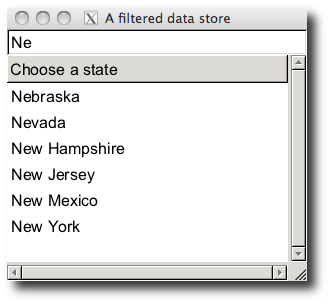
\includegraphics[width=.45\textwidth]{ex-RGtk2-filtered}
  \caption{Example of a data store filtered by values typed into a text-entry widget.}
  \label{fig:RGtk2-filtered}
\end{figure}

We use a convenient set of names and create a data frame. The
\code{VISIBLE} column will be added to the \code{rGtkDataFrame}
instance to adjust the visible rows.
\begin{Schunk}
\begin{Sinput}
 df <- data.frame(state.name)
 df$VISIBLE <- rep(TRUE, nrow(df))
 store <- rGtkDataFrame(df)
\end{Sinput}
\end{Schunk}

The filtered store needs to have the column specified that contains
the logical values, in this example it is the last column.
\begin{Schunk}
\begin{Sinput}
 filteredStore <- store$filterNew()
 filteredStore$setVisibleColumn(ncol(df)-1)      # offset
 view <- gtkTreeView(filteredStore)
\end{Sinput}
\end{Schunk}

This example uses just one column, we create a basic view of it below.
\begin{Schunk}
\begin{Sinput}
 vc <- gtkTreeViewColumn()
 cr <- gtkCellRendererText()
 vc$packStart(cr, TRUE)
 vc$setTitle("Col")
 vc$addAttribute(cr, "text", 0)
 QT <- view$insertColumn(vc, 0)
\end{Sinput}
\end{Schunk}

An entry widget will be used to control the filtering. In the
callback, we adjust the \code{VISIBLE} column of the
\code{rGtkDataFrame} instance, to reflect the rows to be shown. When
\code{val} is an empty string, the result \function{grep} is just
\code{TRUE}, so all rows will be shown. The
\code{getModel} method of the filtered store is used, although we
could have passed in that store itself.
\begin{Schunk}
\begin{Sinput}
 e <- gtkEntry()
 ID <- gSignalConnect(e, "changed", function(w, data) {
   val <- w$getText()
   df <- data$getModel()
   values <- df[,1]
   df[, dim(df)[2]] <- sapply(values, function(i) 
                              as.logical(length(grep(val,i))))
 },
                      data=filteredStore)
\end{Sinput}
\end{Schunk}


Figure~\ref{fig:RGtk2-filtered} shows the two widgets placed within a
simple GUI.
\end{example}


%% ping pong
\begin{example}{A widget for variable selection}{ex:RGtk2-pingpong}
This example shows a combination widget that is familiar from other
statistics GUIs. It provides two tree views listing variable names and
has arrows to move variable names from one side to the other. Often
such widgets are used for specifying statistical models. 

\begin{figure}
  \centering
  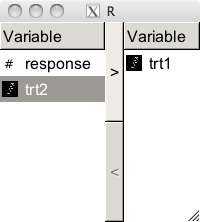
\includegraphics[width=.4\textwidth]{ex-RGtk2-pingpong}
  \caption{An example showing to tree views with buttons to move entries from one to the other. This is a common method for variable selection.}
  \label{fig:RGtk2-pingpong}
\end{figure}


We will use Example~\ref{ex:RGtk2:add-stock-icons}, in particular its
function \code{addToStockIcons}, to add some custom
stock icons to identify the variable type.
\begin{Schunk}
\begin{Sinput}
 nms <- c("factor","numeric")
 fileNms <- c(system.file("images","factor.gif", package="gWidgets"),
              system.file("images","numeric.gif", package="gWidgets"))
 QT <- addToStockIcons(nms, fileNms)
\end{Sinput}
\end{Schunk}

To keep track of the variables in the two tree views we use a single
model. It has a column for all the variable names, a column for the
icon, and two columns to keep track of which variable names are to be
displayed in the respective tree views.
\begin{Schunk}
\begin{Sinput}
 d <- data.frame(varNames=c("response", "trt1", "trt2"),
                 stock.id=c("new-numeric", "new-factor", "new-factor"),
                 leftView  = rep(TRUE, 3),
                 rightView = rep(FALSE, 3),
                 stringsAsFactors=FALSE)
 model <- rGtkDataFrame(d)
\end{Sinput}
\end{Schunk}

We will use a filtered data store to show each tree view.
As the two tree views are identical, except for the rows that are
displayed, we use a function to generate them. The \code{vis.col}
indicates which column in the \code{rGtkDataFrame} object contains the
visibility information. Our tree view packs in both a pixbuf cell
rendererer and a text one.
\begin{Schunk}
\begin{Sinput}
 ## make a view
 makeView <- function(model, vis.col) {
   filteredModel <- model$filterNew()
   filteredModel$setVisibleColumn(vis.col - 1)
   tv <- gtkTreeView(filteredModel)
   tv$getSelection()$setMode("multiple")
   ##
   vc <- gtkTreeViewColumn()
   vc$setTitle("Variable")
   tv$insertColumn(vc, 0)
   ##
   cr <- gtkCellRendererPixbuf()
   vc$PackStart(cr, expand=FALSE)
   cr['xalign'] <- 1
   vc$addAttribute(cr, "stock-id", 1)
   ##
   cr <- gtkCellRendererText()
   vc$PackStart(cr, expand=TRUE)
   cr['xalign'] <- 0
   cr['xpad'] <- 5
   vc$addAttribute(cr, "text", 0)
 
   return(tv)
 }
\end{Sinput}
\end{Schunk}
We know create the tree views and store the selections associated to each.
\begin{Schunk}
\begin{Sinput}
 views <- list()
 views[["left"]] <- makeView(model,3)
 views[["right"]] <- makeView(model,4)
 selections <- lapply(views, gtkTreeViewGetSelection)
\end{Sinput}
\end{Schunk}
We need buttons to move the values left and right, these are stored
in a list for convenience later on.
\begin{Schunk}
\begin{Sinput}
 buttons <- list()
 buttons[["fromLeft"]] <- gtkButton(">")
 buttons[["fromRight"]] <- gtkButton("<")
\end{Sinput}
\end{Schunk}

Our basic GUI is shown in Figure~\ref{fig:RGtk2-pingpong} where the
two tree views are placed side-by-side.
%The basic GUI just lays out the two tree views with the buttons in
%between. We left out command to add scrollwindows etc.

The key handler moves the selected value from one side to the
other. The issue here is that when the view is using filtering the
selection returns values relative to the child model (the filtered
one). In general the methods of the filtered model
\code{convertChildPathToPath} and \code{convertChildIterToIter} will
translate between the two models, but in this case we pass in the
\code{rGtkDataFrame} instance, not the filtered model. So we use the
columns indicating visibility to identify which index is being
referred to. This handler assumes the model and a value indicating the
view (\code{from}) is passed in through the user data.
\begin{Schunk}
\begin{Sinput}
 moveSelected <- function(b, data) {
   model <- data$model
 
   selection <- selections[[data$from]]
   selected <- selection$getSelectedRows()
   if(length(selected$retval)) {
     childRows <- sapply(selected$retval, function(childPath) {
       childRow <- as.numeric(childPath$toString()) + 1
     })
     shownIndices <- which(model[, 2 + data$from])
     rows <- shownIndices[childRows]
 
     model[rows, 2 + data$from] <- FALSE
     model[rows, 2 + (3-data$from)] <- !model[rows, 2 + data$from]
   }
 }
\end{Sinput}
\end{Schunk}
We connect the handler to the \qcode{clicked} signal for the buttons.
\begin{Schunk}
\begin{Sinput}
 IDs <- sapply(1:2, function(i) 
               gSignalConnect(buttons[[i]], signal="clicked", 
                              f=moveSelected,
                              data=list(from=i, model=model)))
\end{Sinput}
\end{Schunk}

We add one flourish, namely ensuring that the arrows are not sensitive
when the corresponding selection is not set. This handler for the
selections is used.
\begin{Schunk}
\begin{Sinput}
 disableButton <- function(sel, data) {
   selected <- sel$getSelectedRows()
   buttons[[data]]$setSensitive(length(selected$retval) != 0)
 }
 IDs <- sapply(1:2, function(i) 
               gSignalConnect(selections[[i]], signal="changed",
                              f=disableButton,
                              data=i))
\end{Sinput}
\end{Schunk}
As the initial state has no selection,  we set the buttons sensitivity accordingly.
\begin{Schunk}
\begin{Sinput}
 QT <- sapply(buttons, function(i) i$setSensitive(FALSE))
\end{Sinput}
\end{Schunk}
 \end{example}

%% editable
% \begin{example}{An editable data frame}{ex:RGtk2-editable-dataframe}
%   \SweaveInput{ex-RGtk2-editable-dataframe}
% \end{example}


%% Tree stores
The \constructor{gtkTreeView} widget displays either list stores or
tree  stores. The difference for the programmer is in the creation of
the data store, not the tree view.

\begin{example}{A simple tree display}{eg:RGtk2-simple-tree}
This example illustrates that the same tree view can display both
rectangular and heirarchical data. The data we use will come from the
\code{Cars93} data set used in Example~\ref{eg:RGtk2:tree-store}. In
that example we defined a simple tree store from a data frame, with a
level for manufacturer and make for different cars. We refer to that
model by \code{tstore} below. 



Now, we make a simple rectangular store for the make information with
the following:

\begin{Schunk}
\begin{Sinput}
 store <- rGtkDataFrame(Cars93[,"Model", drop=FALSE])
\end{Sinput}
\end{Schunk}

The basic view is similar to that for rectangular data already presented.
\begin{Schunk}
\begin{Sinput}
 view <- gtkTreeView()
 vc <- gtkTreeViewColumn()
 vc$setTitle("Make")
 QT <- view$insertColumn(vc, 0)
 cr <- gtkCellRendererText()
 vc$packStart(cr)
 vc$addAttribute(cr, "text", 0)
\end{Sinput}
\end{Schunk}


Finally, we illustrate that the same view can be used with either model:
\begin{Schunk}
\begin{Sinput}
 view$setModel(store)                    # the rectangular store
 view$setModel(tstore)                   # or the tree store
\end{Sinput}
\end{Schunk}
\end{example}

%% ## dynagmic
\begin{example}{Dynamically growing a tree}{eg:RGtk2:tree-dynamic}
This example uses a tree to explore an \R\/ list object, such as what
is returned by one of \R's modelling functions.  As the depth of these
lists is not specified in advance, we use a dynamical approach to
creating the tree store, modifying the tree store when the tree view
is expanded or collapsed.
  


We begin by defining a function that gets the ``children'' of a list
object. For a level of the list, this function returns the named
components, their class and a logical indicating if the component is
recursive.
\begin{Schunk}
\begin{Sinput}
 getChildren <- function(path=character(0)) {
   
   pathToObject <- function(path) {      
     x <- try(eval(parse(text=paste(path,collapse="$")),
                   envir=.GlobalEnv),silent=TRUE)
     if(inherits(x,"try-error")) {
       cat(sprintf("Error with %s",path))
       return(NA)
     }
     return(x)
   }
 
   theChildren <- function(path) {
     if(length(path) == 0)
       ls(envir=.GlobalEnv)
     else
       names(pathToObject(path))
   }
   hasChildren <- function(obj) is.recursive(obj) && !is.null(names(obj))
   
   getType <- function(obj) head(class(obj), n=1)
 
   children <- theChildren(path)
   objs <- sapply(children,function(i) pathToObject(c(path,i)))
   d <- data.frame(children=children,
                   class=sapply(objs, getType),
                   offspring=sapply(objs, hasChildren))
   ## filter out Gtk ones
   ind = grep("^Gtk", d$class)
   if(length(ind) == 0) return(d) else return(d[-ind,])
 }
\end{Sinput}
\end{Schunk}

This function is used to add the children to a tree store.
\begin{Schunk}
\begin{Sinput}
 addChildren <- function(store, children, parentIter=NULL) {
   if(nrow(children) == 0) 
     return(NULL)
   for(i in 1:nrow(children)) {
     iter <- store$append(parent=parentIter)$iter
     ## use last column to indicate logical
     sapply(1:(ncol(children) - 1), function(j)              
            store$setValue(iter, column=j-1, children[i,j]))
     ## Add a branch if there are children
     ## no better way, as this adds an extra blank line
     ## we remove ir later.
     if(children[i, "offspring"])
       store$append(parent=iter)
   }
 }
\end{Sinput}
\end{Schunk}

The various callbacks for the tree view pass back the view and a tree
path. We define some functions to relate these values with iterators.
\begin{Schunk}
\begin{Sinput}
 tpathToPIter <- function(view, tpath) {
   ## view$getModel -- sstore, again store
   sstore <- view$getModel()
   store <- sstore$getModel()
   uspath <- sstore$convertPathToChildPath(tpath)
   p.iter <- store$getIter(uspath)$iter
   return(p.iter)
 }
\end{Sinput}
\end{Schunk}

A ``path'' is made up of the names of each component that makes up an
element in the list. This function returns the path for a component
specified by its iterator.
\begin{Schunk}
\begin{Sinput}
 iterToPath <- function(view, iter) {
   sstore <- view$getModel()
   store <- sstore$getModel()
   string <- store$getPath(iter)$toString()
   indices <- unlist(strsplit(string,":"))
   thePath <- c()
   for(i in seq_along(indices)) {
     path <- paste(indices[1:i],collapse=":")
     iter <- store$getIterFromString(path)$iter
     thePath[i] <- store$getValue(iter,0)$value
   }
   return(thePath[-1])
 }
\end{Sinput}
\end{Schunk}

Now we can begin defining our tree store. This example allows sorting,
so calls the \constructor{gtkTreeModelSortNewWithModel} function.
\begin{Schunk}
\begin{Sinput}
 store = gtkTreeStore(rep("gchararray",2))
 sstore = gtkTreeModelSortNewWithModel(store)
\end{Sinput}
\end{Schunk}

We set an initial root.
\begin{Schunk}
\begin{Sinput}
 iter <- store$append(parent=NULL)$iter
 store$setValue(iter,column=0,"GlobalEnv")
 store$setValue(iter,column=1,"")
 iter <- store$append(parent=iter)
\end{Sinput}
\end{Schunk}
The call of \method{append}{gtkTreeStore} is used to allow the object
to have an expandable icon. 


Now to define the tree view. We allow multiple selection, as an illustration.
\begin{Schunk}
\begin{Sinput}
 view = gtkTreeViewNewWithModel(sstore)
 sel = view$getSelection()
 sel$setMode(GtkSelectionMode["multiple"])
\end{Sinput}
\end{Schunk}

The view will have two similar columns.
\begin{Schunk}
\begin{Sinput}
 ## add two cell renderers -- 1 for name, 1 for type
 nms <- c("Variable name","type")
 for(i in 1:2) {
   cr <- gtkCellRendererText()
   vc <- gtkTreeViewColumn()
   vc$setSortColumnId(i-1) # allow sorting
   vc$setResizable(TRUE)
   vc$setTitle(nms[i])
   vc$packStart(cr,TRUE)
   vc$addAttribute(cr,"text",i-1)
   view$insertColumn(vc, i-1)
 }
\end{Sinput}
\end{Schunk}

We put the tree view widget into a basic GUI.
\begin{Schunk}
\begin{Sinput}
 sw <- gtkScrolledWindow()
 sw$setPolicy("automatic","automatic")
 sw$add(view)
 w <- gtkWindow()
 w$setTitle("Tree view")
 w$add(sw)
\end{Sinput}
\end{Schunk}


At this point, we can see the first level, but nothing will happen if
we click on the trigger icon. We need to specify a handler for the
\code{row-expanded} signal. The odd thing here, is that we appended an
fake child, so that an expand icon would appear. In this, we remove it.

\begin{Schunk}
\begin{Sinput}
 ID <- gSignalConnect(view,signal="row-expanded",
                      f = function(view, iter, tpath, user.data) {
                        store <- user.data
                        p.iter <- tpathToPIter(view, tpath)
                        path <- iterToPath(view, p.iter)
                        children = getChildren(path)
                        addChildren(store, children, parentIter=p.iter)
                        ## remove errant 1st offspring. See addChildren
                        ci <- store$iterChildren(p.iter)
                        if(ci$retval) store$remove(ci$iter)
                      },
                      data=store)
\end{Sinput}
\end{Schunk}

Since the new data is generated when the row is expanded, we need
to remove the old data when the row is closed.
\begin{Schunk}
\begin{Sinput}
 ID <- gSignalConnect(view,signal="row-collapsed",
                   f = function(view, iter, tpath, user.data) {
                     store <- user.data
                     p.iter <- tpathToPIter(view,tpath)
 
                     n = store$iterNChildren(p.iter)
                     if(n > 1) { ## n=1 gets removed when expanded
                       for(i in 1:(n-1)) {
                         child.iter = store$iterChildren(p.iter)
                         if(child.iter$retval)
                           store$remove(child.iter$iter)
                       }
                     }
                   }, data=store)
\end{Sinput}
\end{Schunk}

Finally, this handler simply shows how to get the value (or values if
multiple selection is okay). 
\begin{Schunk}
\begin{Sinput}
 ID <- gSignalConnect(view,signal="row-activated",
                      f = function(view, tpath, tcol) {
                        p.iter <- tpathToPIter(view, tpath)
                        path <- iterToPath(view, p.iter)
                        sel <- view$getSelection()
                        out <- sel$getSelectedRows()
                        if(length(out) == 0) return(c()) # nothing
                        vals <- c()
                        for(i in out$retval) {  # multiple selections
                          iter <- out$model$getIter(i)$iter
                          vals <- c(vals, out$model$getValue(iter,0)$value)
                        }
                        print(vals)      # Insert Real Function Here
                      })
\end{Sinput}
\end{Schunk}



\end{example}
%% % ## mapes a list, shows how to update text view
% \SweaveInput{ex-RGtk2-tree-show}






\chapter{RGtk2: Menus and Dialogs}
\label{sec:RGtk2-menus}
% Menus in RGtk2

\section{Actions}
\label{sec:RGtk2:actions}

Actions are a means to create reusable representations for some action
to be initiated. The \constructor{gtkAction} constructor creates
actions, taking arguments \argument{name}{gtkAction},
\argument{label}{gtkAction} (what gets shown),
\argument{tooltip}{gtkAction}, and \argument{stock.id}{gtkAction}.
The act associated with an action is specified by adding a callback to
the \signal{activate} signal.

Actions are connected to widgets, through the method
\method{connectProxy}{gtkAction}. For buttons, the stock id
information must be added to the button through the button's
\code{setImage} method. The action's \method{createIcon}{gtkAction}
method, with argument coming from a value of \code{GtkIconSize}, will
return the needed image.

Actions can have their \code{sensitivity} property adjusted through
their \method{SetSensitive}{gtkAction} method. This will propogate to
all the widgets the action has a proxy connection with.


\begin{example}{An action object}{ex:RGtk2-action-object}
A basic action can be defined as follows:
\begin{Schunk}
\begin{Sinput}
 a <- gtkAction(name="ok", label="_Ok", tooltip="An OK button", stock.id="gtk-ok")
 ID <- gSignalConnect(a, "activate", f = function(w, data) {
   print(a$GetName())                    # of some useful thing
 })
\end{Sinput}
\end{Schunk}
To connect the action to a button, is straightforward.
\begin{Schunk}
\begin{Sinput}
 b <- gtkButton()
 a$connectProxy(b)
\end{Sinput}
\end{Schunk}

The image must be manually placed, which is facilitated by methods for
the button and the action object.
\begin{Schunk}
\begin{Sinput}
 b$setImage(a$createIcon('button')) # GtkIconSize value
\end{Sinput}
\end{Schunk}

\end{example}
\section{Menus}
\label{sec:RGtk2:menus}

A menu allows access to the GUI's actions in an organized way. This
organization relies on a choice of top-level menu items, their
possible submenus, and grouping within the same level of a
menu. Menubars are typically nested. Toolbars allow access more
quickly to common actions, but do not allow for nesting.

Menubars and popup menus  may be constructed by appending each menuitem
and submenu separately, as illustrated below. An alternative, using a
UI manager, is described in a subsequent section,

To specify a menubar step-by-step consists of defining a top-level
menu bar (\command{gtkMenuBar}). To a menu bar we append menu
items. Menu items may have sub menus (\constructor{gtkMenu}) appended, which gives
the heirarchical nature of a menu. Popup menus are similar, although begin with a \constructor{gtkMenu} instance.  

%% attach
\paragraph{Building the the menu}
Submenus and added to a menu item through the
\method{SetSubMenu}{gtkMenuItem} method. Menu items are added to a
menu through the methods
\method{Append}{gtkMenuShell}; \method{Prepend}{gtkMenuShell}; and
\method{Insert}{gtkMenuShell}, the latter requiring an index where the
insertion is to take place, with 0 being the same as \code{Prepend},
in addition to the child. After a child is added, the method
\method{ReorderChild}{gtkMenuShell} can be used to move it to a new
position ($0$-based). Menuitems are not typically removed, rather they
are disabled through their \code{SetSensitive} method, but if desired
their \method{Show}{gtkWidget} and \method{Hide}{gtkWidget} methods
can be used to stop them from being drawn.

%% Menu itmes
%% From API docs for gtkAccelGroup
% Note that accelerators are different from mnemonics. Accelerators are shortcuts for activating a menu item; they appear alongside the menu item they're a shortcut for. For example "Ctrl+Q" might appear alongside the "Quit" menu item. Mnemonics are shortcuts for GUI elements such as text entries or buttons; they appear as underlined characters. See gtk_label_new_with_mnemonic(). Menu items can have both accelerators and mnemonics, of course. 

\paragraph{Menu items}
Menu items represent actions to be taken and are created by several
different constructors.  A basic menu item is created by
\constructor{gtkMenuItem}. The argument \argument{label}{gtkMenuItem}
allows one to specify the label at construction time. The related
constructor, \constructor{gtkMenuItemNewWithMnemonic} also allows the
specification of a label, only underscores within the string specify
the mnemonic for the menu item.  To group menu items, one use
separators (\constructor{gtkSeparatorMenuItem}).

A menu item for a \code{gtkAction} object can be created by its
\method{createMenuItem}{gtkAction} method. For window managers that
display them, any icon specified the action's \code{stock.id} argument
will be displayed.


To add a different image in the menu bar, the
\constructor{gtkImageMenuItem} can be used. Although, the
\argument{stock.id}{gtkImageMenuItem} argument can be used to specify
the icon, we don't use this, as then the argument
\argument{accel.group}{gtkImageMenuItem} must be specified. An
accelerator group defines a set of keyboard shortcuts to initiate
actions, such as a \kbd{Ctrl+Q} to quit. (A mnemonic is a keyboard
shortcut to indicate a GUI element). We don't discuss creating those
here (they are given in the UI manager example). If instead of the
\code{stock.id} argument, just the \code{label} is specified for the
image menu item, the image can be added later through the
\method{SetImage}{gtkImageMenuItem} method. This takes an image object
for an argument. 

A check button menu item can be created by
\constructor{gtkCheckMenuItem}. This menu item shows a check box when
the \code{active} state for the menu is set. The default is not
active. Use the \method{GetActive}{gtkCheckMenuItem} to test if the
state is active or not.  It may be best to set this state to active,
so the user can identify that the item is a toggle (use the method
\code{SetActive(TRUE)}. When the user clicks on the menu item, the
\signal{toggled} signal is emitted.

\begin{example}{A basic menu bar}{eg:Rgtk2-Basic}
We illustrate how to make a basic menu bar with a plain item, an
item with an icon, and check item. Our GUI, just adds a menubar to a
top-level window.

We create top-level menubar and a menu item for our top level File entry with a mnemonic.
\begin{Schunk}
\begin{Sinput}
 mb <- gtkMenuBar()
 fileMi <- gtkMenuItemNewWithMnemonic(label="_File")
 mb$append(fileMi)
\end{Sinput}
\end{Schunk}

For the menu item we attach a submenu.
\begin{Schunk}
\begin{Sinput}
 fileMb <- gtkMenu()
 fileMi$setSubmenu(fileMb)
\end{Sinput}
\end{Schunk}
We now define some menu items. First a basic one:
\begin{Schunk}
\begin{Sinput}
 open <- gtkMenuItem(label="open")
\end{Sinput}
\end{Schunk}

Next we show how an \code{gtkAction} item can define a menuitem.
\begin{Schunk}
\begin{Sinput}
 saveAction <- gtkAction("save", "save", "Save object", "gtk-save")
 save <- saveAction$CreateMenuItem()
\end{Sinput}
\end{Schunk}

This illustrates how to add an image to the menu bar using a stock icon. The size specification is important to get the correct look.
\begin{Schunk}
\begin{Sinput}
 quit <- gtkImageMenuItem(label="quit")
 quit$setImage(gtkImageNewFromStock("gtk-quit", size=GtkIconSize["menu"]))
\end{Sinput}
\end{Schunk}

A simple check menu item can be created, as follows:
\begin{Schunk}
\begin{Sinput}
 happy <- gtkCheckMenuItem(label="happy")
 happy$setActive(TRUE)
\end{Sinput}
\end{Schunk}

These items are appended in the desired order, by
\begin{Schunk}
\begin{Sinput}
 Qt <- sapply(list(open, save, happy, gtkSeparatorMenuItem(), quit), function(i) {
        fileMb$append(i)
      })
\end{Sinput}
\end{Schunk}
We specify a handler for the toggle button
\begin{Schunk}
\begin{Sinput}
 ID <- gSignalConnect(happy, "toggled", function(b,data) {
   if(b$getActive())
     print("User is now happy")
 })
\end{Sinput}
\end{Schunk}
For the other  items, we specify a generic action for the \signal{activate} signal.
\begin{Schunk}
\begin{Sinput}
 QT <- sapply(list(open, quit, saveAction), function(i) 
        gSignalConnect(i, "activate", f=function(mi, data) {
          cat("item selected\n")
        })
        )
\end{Sinput}
\end{Schunk}

We make as simple GUI for the menubar.
\begin{Schunk}
\begin{Sinput}
 w <- gtkWindow(show=FALSE)
 w['title'] <- "Menubar example"
 w$add(mb)
 w$ShowAll()
\end{Sinput}
\end{Schunk}
\end{example}

\begin{example}{Popup menus}{ex:RGtk2-popup-menus}
To illustrate popup menus, we show how define a one and connect it to
a third-mouse click. We start with a \code{gtkMenu} instance, to which we add some items.
\begin{Schunk}
\begin{Sinput}
 popup <- gtkMenu()                       # top level
 for(i in c("cut","copy","----","paste")) {
   if(i == "----")
     popup$append(gtkSeparatorMenuItem())
   else
     popup$append(gtkMenuItem(i))
 }
\end{Sinput}
\end{Schunk}

This menu will be shown by \code{gtkMenuPopup}. This function is
called with the menu, some optional arguments for placement, and
values for the button that was clicked and the time of
activation. These values can be retrieved from the second argument of
the callback (a \code{GdkEvent}), as shown.
\begin{Schunk}
\begin{Sinput}
 b <- gtkButton("Click me with right mouse button")
 w <- gtkWindow(); w$setTitle("Popup menu example")
 w$add(b)
 ID <- gSignalConnect(b,"button-press-event",
                     f = function(w, e, userData) {
                       if(e$getButton() == 3 ||
                          (e$getButton() == 1 && # a mac
                           e$getState() == GdkModifierType['control-mask'])
                          ) {
                         gtkMenuPopup(userData$mb,
                                      button = e$getButton(),
                                      activate.time = e$getTime())
                         }
                       return(FALSE)
                     },
                     data=list(mb=popup)
                     )
\end{Sinput}
\end{Schunk}

The above will popup a menu, but until we bind to the \code{activate}
signal, nothing will happen when a menu item is selected. Below we
supply a stub for sake of illustration. The children of a popup menu
are the menu items, including the separator which we avoid.
\begin{Schunk}
\begin{Sinput}
 IDs <- sapply(popup$getChildren(), function(i) {
   if(!inherits(i, "GtkSeparatorMenuItem")) # skip these
     gSignalConnect(i, "activate",
                    f = function(w, data) print("replace me"))
 })
\end{Sinput}
\end{Schunk}
\end{example}


The above can easily be automated. The menubar widget in
\pkg{gWidgetsRGtk2} simply maps a list with named components to the
above, by setting menu items for each top-level component, submenus for
each component that contains children, and menu items for components
that do not have children. However, the next approach is preferred for
larger menubars, as it separates out the presentation from the actions.

\section{Toolbars}
\label{sec:RGtk2:toolbars}

Toolbars are like menubars only they only contain actions, there are
no submenus. Toolbar objects are constructed by
\constructor{gtkToolbar}. The placement of the widget at the top of a
top-level window is done by the programmer. Toolbar items are added to
the toolbar using the \method{Add}{gtkContainer} method. Once added,
items can be referred to by index using the \code{[[} method.

Toolbar items have some common properties. The buttons are comprised
of an icon and text, and the style of their layout is specified by the
toolbar method \method{SetStyle}{gtkToolbar}, with values coming from
the \code{GtkToolbarStyle} enumeration. Toolbar items can have a
tooltip set for them through the methods
\method{SetTooltipText}{gtkToolItem} or
\method{SetTooltipMarkup}{gtkToolItem}, the latter if PANGO markup is
desired. Toolbar items can be disabled, through the method \method{SetSensitive}{gtkWidget}.

The items can be one of a few different types. A stock toolbar item is
constructed by \constructor{gtkToolbarButtonNewFromStock}, with the
stock id as the argument. The constructor
\constructor{gtkToolbarButton} creates a button that can have its
label and icon value set through methods
\method{SetLabel}{gtkToolbarButton} and
\method{SetIconWidget}{gtkToolbarButton}. Additionally, there are
methods for setting a tooltip or specifying a stock id after
construction. A toggle button, which toggles between looking depressed
or not when clicked is created by \constructor{gtkToggleToolButton} or \constructor{gtkToggleToolButtonNewFromStock}.
Additionally there are constructors to place menus
(\constructor{gtkMenuToolButton}) and radio groups (\constructor{gtkRadioToolButton}).
  
% signale
The \code{clicked} signal is emitted when a toolbar button is
pressed. For the toggle button, the \code{toggle} signal is emitteed. Other



\begin{example}{Basic toolbar usage}{ex:RGtk2-basic-toolbar}
We illustrate with a toolbar, whose buttons are produced in various ways.
\begin{Schunk}
\begin{Sinput}
 tb <- gtkToolbar()
\end{Sinput}
\end{Schunk}
A button with a stock icon is produced by a call to the appropriate constructor.
\begin{Schunk}
\begin{Sinput}
 b1 <-  gtkToolButtonNewFromStock("gtk-open") 
 tb$add(b1)
\end{Sinput}
\end{Schunk}
To use a custom icons, requires a few steps.
\begin{Schunk}
\begin{Sinput}
 f <- system.file("images/dataframe.gif", package="gWidgets")
 image <- gtkImageNewFromFile(f)
 b2 <- gtkToolButton()
 b2$setIconWidget(image)
 b2$setLabel("Edit")
 tb$add(b2)
\end{Sinput}
\end{Schunk}
Adding a toggle button also is just a matter of calling the
appropriate constructor. In this, example we illustrate how to
initiate the callback only when the button is depressed.
\begin{Schunk}
\begin{Sinput}
 b3 <- gtkToggleToolButtonNewFromStock("gtk-fullscreen")
 tb$add(b3)
 QT <- gSignalConnect(b3, "toggled", f=function(button, data) {
   if(button$getActive())
     cat("toggle button is depressed\n")
   })
\end{Sinput}
\end{Schunk}
We give the other buttons a simple callback when clicked:
\begin{Schunk}
\begin{Sinput}
 QT <- sapply(1:2, function(i) gSignalConnect(tb[[i]], "clicked", function(button, data) {
   cat("You clicked", button$getLabel(), "\n")
 }))
\end{Sinput}
\end{Schunk}

\begin{Schunk}
\begin{Sinput}
 w <- gtkWindow(show=FALSE)
 w['title'] <- "Toolbar example"
 g <- gtkVBox()
 w$add(g)
 g$packStart(tb, expand=FALSE)
 g$packStart(gtkLabel("filler"), expand=TRUE, fill=TRUE)
 w$showAll()
\end{Sinput}
\end{Schunk}
\end{example}

\section{Statusbars}
\label{sec:RGtk2:statusbars}

In \GTK, a statusbar is constructed through by the
\constructor{gtkStatusbar} function. Statusbars must be placed at the
bottom of a top-level window by the programmer. In \GTK, a statusbar
keeps various stacks of messages for display. One adds a message to
display for given stack through the \method{Push}{gtkStatusbar} method
by specifying first an integer value for \code{context.id} and a
message. To pop the top message on a stack and display the next, the
method \method{Pop}{gtkStatusbar} method is available.


\section{UI Managers}
\label{sec:RGtk2:UIManager}


A GUI is designed around actions that are accessible through the
menubar and the toolbar. The notion of a \dfn{user interface manager}
(\acronym{UI} manager) separates out the definitions of the actions
from the user interface. The steps required to use \GTK's UI manager
are 
\begin{enumerate}
\item define a UI manager,
\item  set up an accelarator group for
keyboard shortcuts,
\item define our actions,
\item create action groups to
specify the name, label (with possible mnuemonic), keyboard
accelerator, tooltip, icon and callback for the graphical elements
that call the action,
\item specify where the menu items and toolbar
items will be placed,
\item connect the action group to the UI manager,
and finally
\item display the widgets.
\end{enumerate}

We show by an example how this is done. 

\begin{example}{UI Manager example}{ex:RGtk2:UImanager}
We define the UI manager as follows

\begin{figure}
  \centering
  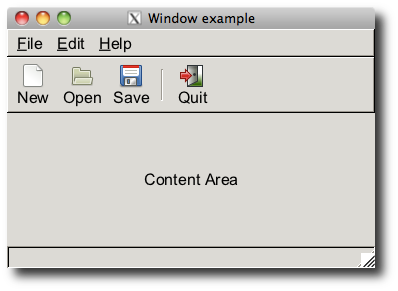
\includegraphics[width=.6\textwidth]{ex-RGtk2-UI}
  \caption{A GUI made using a UI manager to layout the menubar and toolbar.}
  \label{fig:RGtk2-UI}
\end{figure}


\begin{Schunk}
\begin{Sinput}
 uimanager = gtkUIManager()
\end{Sinput}
\end{Schunk}

Our actions either open a dialog to gather more information or issue a
command. A \class{GtkAction} element is passed to the action. We
define a stub here, that simply updates a \code{gtkStatusbar}
instance, defined below.
\begin{Schunk}
\begin{Sinput}
 someAction <- function(action,...) 
   statusbar$push(statusbar$getContextId("message"), action$getName())
 Quit <- function(...) win$destroy()
\end{Sinput}
\end{Schunk}

To show how we can sequentially add interfaces, we break up our action
group definitions into one for ``File'' and ``Edit'' and another one
for ``Help.'' The key is the list defining the entries. Each component
specifies (in this order) the name; the icon; the label, with
\code{\_} specifying the mnemonic; the keyboard accelerator, with
\code{<control>}, \code{<alt>}, \code{<shift>} as possible prefixes, a
tooltip, which may not work with the \R\/ event loop, and finally the
callback. Empty values can be defined as \code{NULL} or, except for
the callback, an empty string.


\begin{Schunk}
\begin{Sinput}
 firstActionGroup = gtkActionGroup("firstActionGroup")
 firstActionEntries = list(
   ## name,ID,label,accelerator,tooltip,callback
   file = list("File",NULL,"_File",NULL,NULL,NULL),
   new = list("New","gtk-new","_New","<control>N","New document",someAction),
   sub = list("Submenu",NULL,"S_ub",NULL,NULL,NULL),
   open = list("Open","gtk-open","_Open","<ctrl>0","Open document",someAction),
   save = list("Save","gtk-save","_Save","<alt>S","Save document",someAction),
   quit = list("Quit","gtk-quit","_Quit","<ctrl>Q","Quit",Quit),
   edit = list("Edit",NULL,"_Edit",NULL,NULL,NULL),
   undo = list("Undo","gtk-undo","_Undo","<ctrl>Z","Undo change",someAction),
   redo = list("Redo","gtk-redo","_Redo","<ctrl>U","Redo change",someAction)
 )
\end{Sinput}
\end{Schunk}
We now add the actions to the action group, then add this action group
to the first spot in the UI manager.
\begin{Schunk}
\begin{Sinput}
 QT <- firstActionGroup$addActions(firstActionEntries)
 uimanager$insertActionGroup(firstActionGroup,0) # 0 -- first spot
\end{Sinput}
\end{Schunk}

The ``Help'' actions we do a bit differently. We define a ``Use
tooltips'' mode to be a toggle, as an illustration of that feature. One can also
incorporate radio groups, although this is not shown.

\begin{Schunk}
\begin{Sinput}
 helpActionGroup = gtkActionGroup("helpActionGroup")
 helpActionEntries = list(
   help = list("Help","","_Help","","",NULL),
   about = list("About","gtk-about","_About","","",someAction)
   )
 QT <- helpActionGroup$AddActions(helpActionEntries)
\end{Sinput}
\end{Schunk}

A toggle is defined with \command{gtkToggleAction} which has signature
in a different order than the action entry. Notice, we don't have an
icon, as the toggled icons is used.  To add a callback, we connect to
the \code{toggled} signal of the action element. This callback allows
for user data, as illustrated.

\begin{Schunk}
\begin{Sinput}
 toggleAction <- gtkToggleAction("UseTooltips",label="_Use tooltips",
                                 tooltip="Use tooltips ")
 toggleAction$setActive(TRUE)            # initially set
 ID <- gSignalConnect(toggleAction,signal = "toggled",
                     f=function(ta,userData) cat(userData,ta$getName(),"\n"),
                     data="toggled")
 helpActionGroup$addAction(toggleAction)
\end{Sinput}
\end{Schunk}
We insert the help action group in position 2.
\begin{Schunk}
\begin{Sinput}
 uimanager$insertActionGroup(helpActionGroup,1)
\end{Sinput}
\end{Schunk}
The \code{SetActive} method can set the state, use \code{GetActive} to
retrieve the state.


Our UI Manager's layout is specified in a file. The file uses XML to
specify where objects go. The structure of the file can be grasped
quickly from the example. Each entry is wrapped in \code{ui} tags. The
type of UI is either a \code{menubar}, \code{toolbar}, or
\code{popup}.  The \code{name} properties are used to reference the
widgets later on.  Menuitems are added with a \code{menuitem} entry
and toolbar items the \code{toolitem} entry. These have an
\code{action} value and an optional name (defaulting to the
\code{action} value). The \code{separator} tags allow for some
formatting.  The nesting of the menuitems is achieved using 
the \code{menu} tags. A \code{placeholder} tag can be used to add
entries at a later time.

\begin{verbatim}
<ui>
  <menubar name="menubar">
    <menu name="FileMenu" action="File">
      <menuitem name="FileNew" action="New"/>
      <menu action="Submenu">
	<menuitem name="FileOpen" action="Open" />
      </menu>
      <menuitem name="FileSave" action="Save"/>
      <separator />
      <menuitem name="FileQuit" action="Quit"/>
    </menu>
    <menu action="Edit">
      <menuitem name="EditUndo" action="Undo" />
      <menuitem name="EditRedo" action="Redo" />
    </menu>
    <menu action="Help">
      <menuitem action="UseTooltips"/>
      <menuitem action="About"/>
    </menu>
  </menubar>
  <toolbar name="toolbar">
    <toolitem action="New"/>
    <toolitem action="Open"/>
    <toolitem action="Save"/>
    <separator />
    <toolitem action="Quit"/>
  </toolbar>
</ui>
\end{verbatim}
%\VerbatimInput{ex-menus.xml}

This file is loaded into the UI manager as follows
\begin{Schunk}
\begin{Sinput}
 id <- uimanager$addUiFromFile("ex-menus.xml")
\end{Sinput}
\end{Schunk}

The \code{id} value can be used to merge and delete UI components, but
this is not illustrated here. The menus can also be loaded from strings.

Now we can setup a basic window template with menubar, toolbar, and
status bar. We first get the three main widgets. We use the names from
the UI layout to get the widgets through the \command{GetWidget}
method of the UI manager. The menubar and toolbar are returned as
follows, for our choice of names in the XML file.
\begin{Schunk}
\begin{Sinput}
 menubar <- uimanager$getWidget("/menubar")
 toolbar <- uimanager$getWidget("/toolbar")
\end{Sinput}
\end{Schunk}
The statusbar is constructed with
\begin{Schunk}
\begin{Sinput}
 statusbar <- gtkStatusbar()
\end{Sinput}
\end{Schunk}
Statusbars have a simple API. The \method{push} method, as used in the
definition of the callback \code{f}, is used to add new text to the
statusbar. The \code{pop} method reverts to the previous message.


Now we define a top-level window and attach a keyboard accelerator
group to the window so that when the window has the focus, the
specified keyboard shortcuts can be used.

\begin{Schunk}
\begin{Sinput}
 win <- gtkWindow(show=TRUE)
 win$setTitle("Window example")
 accelgroup = uimanager$getAccelGroup()  # add accel group
 win$addAccelGroup(accelgroup)
\end{Sinput}
\end{Schunk}


Now it is a simple matter of packing the widgets into a box.
\begin{Schunk}
\begin{Sinput}
 box <- gtkVBox()
 win$add(box)
 box$packStart(menubar, expand=FALSE, fill=FALSE,0)
 box$packStart(toolbar, expand=FALSE, fill= FALSE,0)
 contentArea = gtkVBox()
 box$packStart(contentArea, expand=TRUE, fill=TRUE,0)
 contentArea$packStart(gtkLabel("Content Area"))
 box$packStart(statusbar, expand=FALSE, fill=FALSE, 0)
\end{Sinput}
\end{Schunk}

The redo feature should only be sensitive to mouse events after a user
has undone an action and has not done another. To set the sensitivity
of a menu item is done through the \method{SetSensitive} method called
on the widget. We again retrieve the menuitem or toolbar item widgets
through their names.

\begin{Schunk}
\begin{Sinput}
 uimanager$getWidget("/menubar/Edit/EditRedo")$setSensitive(FALSE)
\end{Sinput}
\end{Schunk}
To reenable, use \code{TRUE} for the argument to \command{SetSensitive}

We can also use the \method{SetText} method on the menuitems. For
instance, instead of a generic ``Undo'' label, one might want to
change the text to list the most previous action.  The method is not
for the menu item though, but rather a \code{gtkLabel} which is the
first child. We use the list notation to access that.
\begin{Schunk}
\begin{Sinput}
 a <- uimanager$getWidget("/menubar/Edit/EditUndo")
 a[[1]]$setText("Undo add text")
\end{Sinput}
\end{Schunk}
\end{example}


\label{sec:RGtk2:dialogs}
\section{Dialogs}
\label{sec:dialogs}
\GTK\/ comes with a variety of dialogs to create simple, usually
single purpose, popup windows
for the user to interact with.

\subsection{The \code{gtkDialog} constructor}

The constructor \constructor{gtkDialog} creates a basic dialog box,
which is a display containing a top section with optionally an icon, a
message, and a secondary message. The bottom section, the action area,
shows buttons, such as \kbd{yes}, \kbd{no} and/or
\kbd{cancel}. The convenience functions
\constructor{gtkDialogNewWithButtons} and
\constructor{gtkMessageDialog} simplify the construction.

In \GTK\/ dialogs can be modal or not. Thre are a few ways to make a
dialog modal. The method window \method{setModal}{gtkWindow} will do
so, as will passing in a \code{modal} flag to some of the
constructors. These make other GUI elements inactive, but not the \R\/
session. Whereas, calling the \method{run}{gtkDialog} method,
will stop the flow until the dialog is dismissed, The return value can
then be inspected for the action, such as what button was
pressed. These values are from \code{GtkResponseType}, which lists
what can happen.


\paragraph{Basic message dialogs} The \constructor{gtkMessageDialog} has
an argument \argument{parent}{gtkMessageDialog}, to specify a parent
window the dialog should appear relative to. The
\argument{flags}{gtkMessageDialog} argument allows one to specify
values (from \code{GtkDialogFlags}) of \code{destroy-with-parent} or
\code{modal}. The \argument{type}{gtkMessageDialog} is used to specify
the message type, using a value in \code{GtkMessageType}. The
\argument{buttons}{gtkMessageDialog} is used to specify which buttons
will be drawn. The message is the following argument. The dialog has a
\code{secondary-text} property that can be set to give a secondary message.

\begin{Schunk}
\begin{Sinput}
 w <- gtkWindow()
 w['title'] <- "Parent window"
 dlg <- gtkMessageDialog(parent=w, flags="destroy-with-parent",
                         type="question", buttons="ok",
                         "My message")
 dlg['secondary-text'] <- "A secondary message"
 response <- dlg$run()
 if(response == GtkResponseType["cancel"] || # for other buttons
    response == GtkResponseType["close"] ||
    response == GtkResponseType["delete-event"]) {
   ## pass
 } else if(response == GtkResponseType["ok"]) {
   print("Ok")
 }
 dlg$Destroy()
\end{Sinput}
\end{Schunk}

\paragraph{Making your own dialogs} The \constructor{gtkDialog}
constructor returns a dialog object which can be customized for more
involved dialogs. In the example below, we illustrate how to make a
dialog to accept user input. We use the
\constructor{gtkDialogNewWithButtons}, which allows us to specify a
stock buttosn and a response value. We use standard responses, but could
have used custom ones by specifying a positive integer. The dialog is
a window object containing a box container, which is returned by the
\method{getVbox}{gtkDialog} method. This box has a separator and
button box packed in at the end, we pack in another box at the
beginning below to hold a label and our entry widget. 

When one of the buttons is clicked, the \signal{response} signal is
emitted by the dialog. We connect to this close the dialog.

\begin{Schunk}
\begin{Sinput}
 dlg <- gtkDialogNewWithButtons(title="Enter a value", 
                                parent=NULL, flags=0,
                                "gtk-ok", GtkResponseType["ok"],
                                "gtk-cancel", GtkResponseType["cancel"],
                                show=FALSE)
 g <- dlg$getVbox()                           # content area
 vg <- gtkVBox()
 vg['spacing'] <- 10
 g$packStart(vg)
 vg$packStart(gtkLabel("Enter a value"))
 entry <- gtkEntry()
 vg$packStart(entry)
 ID <- gSignalConnect(dlg, "response", f=function(dlg, resp, user.data) {
   if(resp == GtkResponseType["ok"])
     print(entry$getText())
   dlg$Destroy()
 })
 dlg$showAll()
 dlg$setModal(TRUE)
\end{Sinput}
\end{Schunk}

\subsection{File chooser}
\label{sec:RGtk2:file-chooser}

\GTK\/ has a \class{GtkFileChooser} backend to implement selecting a file
from the file system. The same widget allows one to open or save a
file and select or create
a folder (directory). The action is specified through one of the
\code{GtkFileChooserAction} flags.
This backend presented in various ways through
\constructor{gtkFileChooserDialog}, which pops up a modal dialog;
\constructor{gtkFileChooserButton}, which pops up the dialog when the
button is clicked; and \constructor{gtkFileChooserWidget}, which
creates a widget that can be placed in a GUI to select a file.

The dialog constructor allows one to spcify a title, a parent and an
action. In addition, the dialog buttons must be specified, as with the last
example using \code{gtkDialogNewWithButtons}. 

\begin{example}{An open file dialog}{ex:RGtk2:open-file}
An open file dialog can be created with:

\begin{Schunk}
\begin{Sinput}
 dlg <- gtkFileChooserDialog(title="Open a file", parent=NULL, action="open",
                             "gtk-ok", GtkResponseType["ok"],
                             "gtk-cancel", GtkResponseType["cancel"])
\end{Sinput}
\end{Schunk}

One can use the \code{run} method to make this modal or connect to the
\signal{response} signal. The file selected is found from the file
chooser method \method{getFilename}{gtkFileChooser}. One can enable
multiple selections, by passing
\method{setSelectMultiple}{gtkFileChooser} a \code{TRUE} value. In
this case, the \method{getFilenames}{gtkFileChooser} returns a list of filenames,

\begin{Schunk}
\begin{Sinput}
 ID <- gSignalConnect(dlg, "response", f=function(dlg, resp, data) {
   if(resp == GtkResponseType["ok"]) {
     filename <- dlg$getFilename()
     print(filename)
   }
   dlg$destroy()
 })
\end{Sinput}
\end{Schunk}

For the open dialog, one may wish to specify one or more filters, to narrow the
available files for selection. A filter object is returned by the
\constructor{gtkFileFilter} function.
This object is added to the file chooser, through its
\method{addFilter}{gtkFileChooser} method. The filter has a name
property set through the \method{setName}{gtkFileFilter} method. The
user can select a filter through a combobox, and this provides the
label. To use
the filter, one can add a pattern (\method{addPattern}{gtkFileFilter}),
a MIME type (\method{addMimeType}{gtkFileFilter}), or a custom filter. 

\begin{Schunk}
\begin{Sinput}
 fileFilter <- gtkFileFilter()
 fileFilter$setName("R files")
 dlg$addFilter(fileFilter)
 QT <- sapply(c("*.R", "*.Rdata"), 
              function(i) fileFilter$addPattern(i))
 QT <- sapply(c("text/plain"), 
              function(i) fileFilter$addMimeType(i))
\end{Sinput}
\end{Schunk}
\end{example}

The save file dialog is similar. The
\method{setFilename}{gtkFileChooser} can be used to specify a
default file and \method{setFolder}{gtkFileChooser} can specify an
initial directory. To be careful as to not overwrite an existing file, the
method \method{setDoOverwriteConfirmation}{gtkFileChooser} can be
passed a \code{TRUE} value.

\subsection{Date picker}
\label{sec:RGkt2:date-picker}

A calendar widget is produced by \constructor{gtkCalendar}. This
widget allows selection of a day, month or year. To specify these
values, the properties \code{day}, \code{month} ($0$-$11$), and
\code{year} store these values as integers. One can assign to these
directly, or use the methods
\method{selectDay}{gtkCalendar} and
\method{selectMonth}{gtkCalendar} (no select year method). The method
\method{getData}{gtkCalendar} returns a list with components for the
year, month and day. If there is no selection, the \code{day}
component is $0$.

The widget emits various signals when a selection is changed. The
\signal{day-selected} and \signal{day-selected-double-click} ones are
likely the most useful of these.







% \chapter{\code{cairoDevice}}
% \label{sec:RGtk2-cairoDevice}
% \SweaveInput{cairoDevice}

% \chapter{Using \code{glade} to design GUIs}
% \label{sec:RGtk2-glade}
% \SweaveInput{Glade}

%\section{End of chapter notes}
%\label{sec:RGtk2:end-of-chapter}

% * overview in inst
% * gtk tutorial in R
% * API at http://developer.gimp.org/api/2.0/gtk/
% * ...

% * widget gallery
% http://library.gnome.org/devel/gtk/stable/ch02.html

%  good source: http://developer.gnome.org/doc/GGAD/ggad.html

% * http://gtk.org/documentation.html

% * gtk API
% http://library.gnome.org/devel/gtk/stable/

% * pango manual 
% http://library.gnome.org/devel/pango/stable/PangoMarkupFormat.html

% * Missing discussion on standard dialogs: message, confirmations, etc.
% filebrowser, colors selector, font selector, 

% * Mention history: GIMP; GNOME; DTL RGtk; Michael Lawrence RGtk2
% * Installation: windows; linux; mac OS X

% * Info
% php cookbook good source of info

% DTL examples from omegahat

% pygtk tutorial easier to read than C one (no types specifed)

%%%%%%%%%%%%%%%%%%%%%%%%%%%%%%%%%%%%%%%%%%%%%%%%%%

